\documentclass[12pt, a4paper]{report}
\usepackage[top=3cm, bottom=3cm, left=4cm,right=3cm]{geometry}
\usepackage{setspace} %interlineado
\setlength{\parindent}{7mm} % sangria
\setlength{\parskip}{\baselineskip} %espacio entre parrafos
\usepackage{microtype} %micro-arreglos en los parrafos para que queden mejor justificados
%\renewcommand{\rmdefault}{phv} % Arial
%\renewcommand{\sfdefault}{phv} % Arial
\usepackage{placeins} % ayuda a que las tablas no queden en medio de los textos
\usepackage{tabulary} % ajusta el alto de la tabla
\usepackage{tabularx} % ajusta el ancho de la tabla
\usepackage[font={footnotesize}]{caption} % tamano para la descripcion de las tablas
\usepackage{array}
\usepackage{float}
\usepackage{makecell}
\usepackage{graphicx}
\usepackage{multirow}
\usepackage[spanish,es-tabla,es-lcroman]{babel}
\selectlanguage{spanish}
\usepackage[authoryear,datebegin]{flexbib}
\bibliographystyle{flexbib}
\usepackage{fancyhdr}
%\pagestyle{fancy}
\fancyhead{}
%\fancyfoot{}
\fancyhead[L]{\nouppercase{\leftmark}}
%\fancyfoot[R]{\thepage}
\usepackage{gensymb}
\usepackage{amssymb}
\usepackage{blindtext}
\usepackage{amsmath}
\usepackage{listings}
\usepackage{color}
\usepackage{textcomp}
\definecolor{listinggray}{gray}{0.9}
\lstset{
    tabsize=4,    
%   rulecolor=,
    language=[GNU]C++,
        basicstyle=\scriptsize,
        upquote=true,
        aboveskip={1.5\baselineskip},
        columns=fixed,
        showstringspaces=false,
        extendedchars=false,
        breaklines=true,
        prebreak = \raisebox{0ex}[0ex][0ex]{\ensuremath{\hookleftarrow}},
        frame=single,
        numbers=left,
        showtabs=false,
        showspaces=false,
        showstringspaces=false,
        identifierstyle=\ttfamily,
        keywordstyle=\color[rgb]{0,0,1},
        commentstyle=\color[rgb]{0.026,0.112,0.095},
        stringstyle=\color[rgb]{0.627,0.126,0.941},
        numberstyle=\color[rgb]{0.205, 0.142, 0.73},
%        \lstdefinestyle{C++}{language=C++,style=numbers}’.
}
\lstset{
    tabsize=4,
  language=C++,
  captionpos=b,
  tabsize=3,
  frame=lines,
  numbers=left,
  numberstyle=\tiny,
  numbersep=5pt,
  breaklines=true,
  showstringspaces=false,
  basicstyle=\footnotesize,
%  identifierstyle=\color{magenta},
  keywordstyle=\color[rgb]{0,0,1},
  commentstyle=\color[rgb]{0.3,0.7,0.5},
  stringstyle=\color{red}
}

\newcommand{\membrete}{
	
\includegraphics[width=0.15\textwidth]{./img/escudo-uc.png}~\\[1cm]

	UNIVERSIDAD DE CARABOBO \\	
	Facultad Experimental de Ciencias y Tecnolog\'{i}a\\
	Departamento de Computaci\'{o}n
	\vfill
	\textbf{SOFTWARE PARA EL ESPECTROFOT\'{O}METRO MINISCAN XE PLUS USADO EN EL DIAGN\'{O}STICO DE PATOLOG\'{I}AS DERMATOL\'{O}GICAS EN PACIENTES. CASO DE ESTUDIO: CIMBUC.}
}

\newcommand{\autor}{
	\textbf{Autor:}\\
	Gabriel A. N\'{u}\~{n}ez N.\\
}

\newcommand{\tutores}{
	\textbf{Tutores:} \\
	Prof. Patricia Guerrero \\
	Prof. Harold Vasquez
}

\newcommand{\fechaPortada}{Naguanagua, 
\ifcase \month \or Enero\or Febrero\or Marzo\or Abril\or Mayo\or Junio\or Julio\or Agosto\or Septiembre\or Octubre\or Noviembre\or Diciembre\fi \space de \the\year.}

\newcommand{\proyecto}{
	Software para el MiniScan XE Plus.
}

\newcommand{\nombre}{
	Gabriel N\'{u}\~{n}ez.
}

\newcommand{\fecha}{
	15 de octubre, 2015.
}

\newcommand{\anchotabla}{14cm}

\newcommand{\altocelda}{2pt}

\renewcommand\thechapter{\Roman{chapter}}

\renewcommand\thesection{\arabic{chapter}.\arabic{section}}

\renewcommand\thefigure{\arabic{chapter}.\arabic{figure}}

\renewcommand\thetable{\arabic{chapter}.\arabic{table}}

\usepackage{appendix}
\usepackage{titlesec}
\usepackage{sectsty}
\usepackage{subcaption}
\usepackage{changepage}

\addto\captionsspanish{
  \renewcommand\appendixname{Anexo}
  \renewcommand{\appendixtocname}{Anexos}
  \renewcommand\appendixpagename{Anexos}
}

\chapterfont{\centering}

\begin{document}
	\begin{titlepage}
	\begin{center}
	\membrete
	\vfill
	\textbf{Autor:}\\
	Gabriel A. N\'{u}\~{n}ez N.\\
	\vfill
	\textbf{Tutores:} \\
	Prof. Patricia Guerrero \\
	Prof. Harold Vasquez
	\vfill
	\fecha
	\end{center}
\end{titlepage}
	\begin{titlepage}
	\begin{center}
	\membrete
	\vfill
	Trabajo Especial de Grado\\
	\titulo
	\vfill
	\textbf{Autor:}\\
	Gabriel A. N\'{u}\~{n}ez N.\\
	\vfill
	\textbf{Tutores:} \\
	Prof. Patricia Guerrero \\
	Prof. Harold Vasquez
	\vfill
	Trabajo Especial de Grado presentado ante la ilustre Universidad de Carabobo, como credencial para optar por el t\'{i}tulo de Licenciado en Computaci\'{o}n.
	\vfill
	\fecha
	\end{center}
\end{titlepage}
	\pagenumbering{roman}%numeracion romana
	%\chapter*{Dedicatoria}

A mi abuela, quien me cri\'{o} desde mis cuatro meses de vida, y a quien llamo mam\'{a} desde que tengo uso de la raz\'{o}n. Este trabajo es para ti, representa la culminaci\'{o}n de una etapa donde estuviste presente d\'{i}a a d\'{i}a, gracias por el \'{a}nimo, los consejos y los valores que me has inculcado, por haberme ense\~{n}ado que con Dios de la mano todo se puede, por haber salido adelante conmigo, por haberme hecho el hombre de bien que soy hoy, por todos los sacrificios que hiciste en silencio, y m\'{a}s que nada por todo el amor que has brindado. Te amo mam\'{a}.

\begin{flushright}
	\textbf{Gabriel A. N\'{u}\~{n}ez N.}
\end{flushright}

	%\chapter*{Agradecimientos}

	A Dios, por acompa\~{n}arme en todo momento, por ser mi mejor maestro, y por haberme ayudado a alcanzar esta meta, la culminaci\'{o}n de mi carrera.

	A mi familia, por apoyarme en todo momento, por estar presente para celebrar los logros, compartir la alegr\'{i}a y superar las dificultades.

	A mis amigos, quienes me ayudaron a tomar las cosas con calma, me ayudaron a despejar mi mente innumerables veces, y me dieron el \'{a}nimo necesario para terminar este largo trayecto a tiempo.

	A mi profesora Patricia, por haberme ayudado y aconsejado desde el primero hasta el \'{u}ltimo d\'{i}a de este recorrido, y haberme mostrado que siempre se pueden mejorar las cosas.

	A mi profesor Harold, por saber cu\'{a}ndo exigirme m\'{a}s, ser justo, y mostrarme el nivel de excelencia que puedo alcanzar, a pesar de la distancia.

	Al equipo de profesores e investigadores que hace vida en el CIMBUC, por haberme brindado una experiencia \'{u}nica al trabajar con ellos.

	A la empresa HunterLab, por haber respondido todas mis dudas, y por haberme proporcionado la ayuda que necesit\'{e} e incluso m\'{a}s.


\begin{flushright}
	\textbf{Gabriel A. N\'{u}\~{n}ez N.}
\end{flushright}

	\renewenvironment{abstract}{
  \vspace*{\fill}
  \begin{center}%
    \bfseries\abstractname
  \end{center}}%

\begin{abstract}
	\noindent
El espectrofot\'{o}metro de reflexi\'{o}n difusa, denominado MiniScan XE Plus, es un instrumento de medici\'{o}n utilizado por el Centro de Investigaciones M\'{e}dicas y Biotecnol\'{o}gicas de la Universidad de Carabobo (CIMBUC), que ayuda a los dermat\'{o}logos a establecer diagn\'{o}sticos sobre patolog\'{i}as en la piel de pacientes, de manera precisa y sin necesidad de realizar biopsias. No obstante, el software comercial disponible para la utilizaci\'{o}n de tal instrumento es poco amigable, dif\'{i}cil de utilizar e imposible de modificar y extender. La presente investigaci\'{o}n tiene como objetivo desarrollar un software amigable, modificable y extensible, que se ajuste a las necesidades de los dermat\'{o}logos y que garantice un mejor aprovechamiento del instrumento en cuesti\'{o}n.

	\noindent
	\textbf{Palabras claves:} espectrofot\'{o}metro, an\'{a}lisis bioqu\'{i}mico de la piel, biopsia, software privativo, software libre.
	\vfill
\end{abstract}

\vfill

\selectlanguage{english}
\begin{abstract}
	\noindent
The diffuse reflectance spectrophotometer, called MiniScan XE Plus, is a measurement instrument used by the Medical Research and Biotechnology Center at the University of Carabobo (CIMBUC), which helps dermatologists to establish pathologies diagnoses in the skin of patients precisely, without need for biopsy. However, the available commercial software for the use of such an instrument is unfriendly, difficult to use and impossible to modify and extend. This research aims to develop a friendly, modifiable and expandable software that meets the needs of dermatologists and ensures a better use of the instrument itself.

	\noindent
	\textbf{Keywords:} spectrophotometer, biochemical analysis of the skin, biopsy, privative software, open source software.
	\vfill
\end{abstract}

\selectlanguage{spanish}
	\pagestyle{fancy}%estilo del header
	\pagenumbering{arabic}%numeracion arabica
	\tableofcontents
	\listoffigures
	\listoftables
	\spacing{1.5} % interlineado
	\chapter*{Introducci\'{o}n}

\addcontentsline{toc}{chapter}{Introducci\'{o}n}

	La espectroscop\'{i}a de reflectancia difusa es una t\'{e}cnica \'{o}ptica con la cual es  posible estudiar las propiedades bioqu\'{i}micas y las condiciones estructurales de un tejido biol\'{o}gico. Los instrumentos que emplean t\'{e}cnicas como \'{e}sta son de gran ayuda para los dermat\'{o}logos, raz\'{o}n por la cual tales instrumentos han tomado suma importancia en el \'{a}rea de la medicina dermatol\'{o}gica.

El Centro de Investigaciones M\'{e}dicas y Biotecnol\'{o}gicas de la Universidad de Carabobo (CIMBUC) dispone de un espectrofot\'{o}metro de reflexi\'{o}n difusa denominado MiniScan XE Plus. Este instrumento se utiliza a trav\'{e}s del \'{u}nico software disponible para su manejo, designado HunterLab Universal Software.

El HunterLab Universal Software es un software comercial y privativo que fue descontinuado en el a\~{n}o 2008. Su interfaz gr\'{a}fica de usuario est\'{a} en ingl\'{e}s y contiene m\'{a}s funciones de las necesarias para manejar el instrumento en estudio, lo que lo hace poco amigable y dif\'{i}cil de entender por los dermat\'{o}logos.

Esta investigaci\'{o}n se centr\'{o} en desarrollar un software amigable, modificable y extensible para la utilizaci\'{o}n del MiniScan XE Plus, ajustandose a las necesidades de los dermat\'{o}logos, a fin de sentar una base que permite la realizaci\'{o}n de nuevas investigaciones que conlleven a la implementaci\'{o}n de t\'{e}cnicas que empleen an\'{a}lisis m\'{a}s complejos, y como resultado, diagn\'{o}sticos m\'{a}s completos y diversos sobre patolog\'{i}as dermatol\'{o}gicas presentes en pacientes.

\newpage
\thispagestyle{plain}
	El presente trabajo de investigaci\'{o}n est\'{a} estructurado en cinco cap\'{i}tulos, los cuales son descritos a continuaci\'{o}n.

	El \textbf{cap\'{i}tulo I} describe el contexto de la problem\'{a}tica que motiva el desarrollo de este trabajo de investigaci\'{o}n, se indican los objetivos a cumplir con el mismo y se explican las razones que justifican la necesidad de su realizaci\'{o}n.

	En el \textbf{cap\'{i}tulo II} se presentan los trabajos que anteceden esta investigaci\'{o}n, las observaciones directas realizadas para llevarla a cabo, y se explican las bases te\'{o}ricas que sustentan el desarrollo de las funciones que debe ofrecer el software producto de la misma.

	En el \textbf{cap\'{i}tulo III} se describen la metodolog\'{i}a de investigaci\'{o}n y la metodolog\'{i}a de desarrollo que se emplearon para planificar, dise\~{n}ar y desarrollar el software propuesto en el presente trabajo de investigaci\'{o}n.

	El \textbf{cap\'{i}tulo IV} muestra los resultados que fueron alcanzados en el desarrollo del presente trabajo de investigaci\'{o}n, incluyendo las fases metodol\'{o}gicas, las tecnolog\'{i}as y los recursos utilizados, la interfaz gr\'{a}fica de usuario del software resultante y las pruebas realizadas.

	Finalmente, en el \textbf{cap\'{i}tulo V} se establecen las conclusiones a las que se lleg\'{o} con el presente trabajo de investigaci\'{o}n, y las recomendaciones consideradas a tomar para trabajos futuros, tomando en cuenta dichas conclusiones.

	
	
	\chapter{El Problema}

	\section{Planteamiento del problema}	
El color y la apariencia de la piel humana son importantes en el campo de la medicina. Durante el diagn\'{o}stico de enfermedades de la piel, la observaci\'{o}n cuidadosa y la evaluaci\'{o}n visual del \'{a}rea afectada es siempre el primer paso, y el m\'{a}s importante. Esto es seguido generalmente por una escisi\'{o}n o biopsia por punci\'{o}n, en la que se extrae una muestra de tejido de la piel para un an\'{a}lisis microsc\'{o}pico. La observaci\'{o}n visual suele ser subjetiva, y los pacientes a menudo se someten a cicatrices y dolor durante la biopsia. Por otro lado, las t\'{e}cnicas \'{o}pticas son por lo general no invasivas y sus resultados son a menudo objetivos. Durante el diagn\'{o}stico no invasivo, no se crea ninguna ruptura en la piel, y los pacientes no se someten al dolor ni a cicatrices durante el tratamiento \cite{Bersha}.

Los avances tecnol\'{o}gicos de la actualidad permiten emplear t\'{e}cnicas de \'{o}ptica, capaces de estudiar  las propiedades estructurales y bioqu\'{i}micas del tejido biol\'{o}gico de manera precisa y no invasiva. Los instrumentos que emplean tales t\'{e}cnicas son de gran ayuda para los m\'{e}dicos dermat\'{o}logos, raz\'{o}n por la cual dichos instrumentos han tomado suma importancia en el \'{a}rea de la medicina dermatol\'{o}gica.

Hoy en d\'{i}a existen diferentes tipos de estudios \'{o}pticos in-situ, in-vivo e invitro del tejido biol\'{o}gico, como lo es la espectroscop\'{i}a de reflectancia difusa (ERD). \citeA{Perez} asegura que con esta t\'{e}cnica es  posible estudiar las propiedades bioqu\'{i}micas y las condiciones estructurales de un tejido biol\'{o}gico, analizando la interacci\'{o}n luz-tejido de una manera no invasiva.

En este sentido, el Centro de Investigaciones M\'{e}dicas y Biotecnol\'{o}gicas de la Universidad de Carabobo (CIMBUC) dispone de un espectrofot\'{o}metro de reflexi\'{o}n difusa, denominado MiniScan XE Plus. Este dispositivo fue creado por la empresa HunterLab, la cual lo describe como un instrumento que aplica la t\'{e}cnica de ERD, utilizado para medir la reflectancia de espec\'{i}menes como una funci\'{o}n de longitud de onda.

Ahora bien, el CIMBUC hace uso de este instrumento a trav\'{e}s del \'{u}nico software disponible para su utilizaci\'{o}n, designado HunterLab Universal Software. \'{E}ste es un software comercial y privativo capaz de ejecutarse en sistemas operativos Windows, desde la versi\'{o}n 95 hasta la versi\'{o}n XP. Dicho software contiene funciones que abarcan la utilizaci\'{o}n del MiniScan XE Plus y de otros instrumentos ofrecidos por HunterLab; su interfaz gr\'{a}fica de usuario est\'{a} en ingl\'{e}s, adem\'{a}s de que los resultados que genera no poseen el formato de gesti\'{o}n de informaci\'{o}n de pacientes con el que trabajan los dermat\'{o}logos del CIMBUC. Por \'{u}ltimo, este software fue descontinuado en el a\~{n}o 2008.

Tomando en cuenta lo mencionado anteriormente, se tiene que el HunterLab Universal Software es privativo y est\'{a} descontinuado, por lo tanto no existe la posibilidad de modificarlo ni de extenderlo. Dicho software est\'{a} en ingl\'{e}s y ofrece funciones ajenas al uso exclusivo del MiniScan XE Plus, causando que su interfaz gr\'{a}fica de usuario contenga m\'{a}s opciones de las necesarias para manejar tal instrumento, y que sea dif\'{i}cil de entender por los dermat\'{o}logos. Todo esto sumado al hecho de que los resultados generados por este software deben exportarse y almacenarse manualmente, porque los mismos no poseen el formato con el que trabajan los dermat\'{o}logos, produce la necesidad de contar con asistencia t\'{e}cnica especializada para su debida utilizaci\'{o}n y ralentiza las consultas con los pacientes.

De lo antedicho se desprende que el HunterLab Universal Software posee una interfaz gr\'{a}fica de usuario poco amigable, y el costo del tiempo de capacitaci\'{o}n para su uso correcto podr\'{i}a ser alto. Dicho software no podr\'{a} modificarse ni extenderse, por lo tanto no se fomentar\'{a} el uso del instrumento en cuesti\'{o}n, disminuyendo su potencial. El formato de los resultados de este software convertir\'{a} las consultas de los dermat\'{o}logos con los pacientes en una labor ineficiente en t\'{e}rminos de tiempo. Por \'{u}ltimo, no se fomentar\'{a} el desarrollo de nuevas funciones que utilicen los resultados de dicho software como insumo, sosegando as\'{i} la posibilidad de realizar an\'{a}lisis m\'{a}s complejos, y de proveer resultados que les permitan a los dermat\'{o}logos establecer diagn\'{o}sticos m\'{a}s completos sobre patolog\'{i}as dermatol\'{o}gicas en pacientes.

Motivado a lo anterior, se desarroll\'{o} un software modificable y extensible, con una interfaz gr\'{a}fica de usuario amigable, con funciones para el uso exclusivo del MiniScan XE Plus, que genera resultados relevantes para los dermat\'{o}logos empleando el formato utilizado por ellos para registrar las consultas con los pacientes, y siguiendo los lineamientos de la ingenier\'{i}a del software pertinentes.

Finalmente, con esta investigaci\'{o}n se espera fomentar la utilizaci\'{o}n del \mbox{MiniScan} XE Plus, reducir el tiempo de las consultas con los pacientes, aportar un software sobre el que se puedan desarrollar nuevas investigaciones que conlleven a an\'{a}lisis m\'{a}s complejos, y por \'{u}ltimo, realizar diagn\'{o}sticos m\'{a}s completos y diversos sobre patolog\'{i}as dermatol\'{o}gicas presentes en pacientes.

	\section{Objetivos}

		\subsection{Objetivo general}
	Desarrollar un software para el espectrofot\'{o}metro MiniScan XE Plus, usado en el diagn\'{o}stico de patolog\'{i}as dermatol\'{o}gicas en pacientes, tomando como caso de estudio el CIMBUC.
		\subsection{Objetivos espec\'{i}ficos}
			\begin{itemize}
				\item Investigar el estado del arte relacionado a la investigaci\'{o}n: t\'{e}cnicas de \'{o}ptica y colorimetr\'{i}a, MiniScan XE Plus, HunterLab Universal Software y atributos de calidad del software.
				
				\item Seleccionar una metodolog\'{i}a de investigaci\'{o}n y una metodolog\'{i}a de desarrollo para el nuevo software.
				
				\item Desarrollar el software, siguiendo las metodolog\'{i}as \mbox{seleccionadas}.
				
				\item Realizar las pruebas de funcionalidad y usabilidad al software.
				
				\item Elaborar los manuales de usuario y de instalaci\'{o}n del software.
			\end{itemize}
\newpage
	\section{Justificaci\'{o}n de la investigaci\'{o}n}
	
	Empezando con la interfaz gr\'{a}fica de usuario, \citeA{Sommerville} se\~{n}ala que el dise\~{n}o cuidadoso de la misma es una parte fundamental del proceso de dise\~{n}o general del software. Si un software debe alcanzar su potencial m\'{a}ximo, es fundamental que su interfaz gr\'{a}fica de usuario sea dise\~{n}ada para ajustarse a las habilidades, experiencia y expectativas de sus usuarios previstos. Un buen dise\~{n}o de la interfaz gr\'{a}fica de usuario es cr\'{i}tico para la confiabilidad del software. Muchos de los llamados errores de usuario son causados porque las interfaces gr\'{a}ficas de usuario no consideran las habilidades de los usuarios reales y su entorno de trabajo.

	Dicho lo anterior, el dise\~{n}o de la interfaz gr\'{a}fica de usuario del HunterLab Universal Software es la principal raz\'{o}n por la cual los dermat\'{o}logos requieren de personal t\'{e}cnico especializado que los asista al momento de utilizarlo. Esto porque dicha interfaz est\'{a} en ingl\'{e}s, ofrece funciones que no son necesarias para la utilizaci\'{o}n del MiniScan XE Plus y sus resultados no poseen un formato adecuado. Por estas razones los dermat\'{o}logos perciben este software comercial como no intuitivo, ni auto descriptivo ni amigable, temiendo cometer errores al utilizarlo sin asistencia y generar resultados err\'{o}neos, poniendo en riesgo la fiabilidad del diagn\'{o}stico y, en consecuencia, la salud de los pacientes.

	Con respecto a software de calidad, \citeA{Sommerville} explica lo siguiente: as\'{i} como los servicios que proveen, los productos de software tienen un cierto n\'{u}mero de atributos asociados que reflejan su calidad. Estos atributos no est\'{a}n directamente relacionados con lo que hace el software; m\'{a}s bien, reflejan su comportamiento durante su ejecuci\'{o}n, en la estructura y la organizaci\'{o}n del programa fuente y en la documentaci\'{o}n asociada.

El conjunto espec\'{i}fico de atributos que se esperan de un software de calidad depende obviamente de su aplicaci\'{o}n. En la tabla 1.1 se puede apreciar la generalizaci\'{o}n de estos atributos.

		\begin{table}[t]
			\small
			\caption[Atributos esenciales de un software de calidad]{\textit{Atributos esenciales de un software de calidad} (Fuente: Sommerville, 2005).}
			\centering
			\setlength{\extrarowheight}{\altocelda}
			\begin{tabulary}{\anchotabla}{|c|J|}
				
				\hline
				\thead{\textbf{\small{Caracter\'{i}stica}}} & \thead{\textbf{\small{Descripci\'{o}n}}}\\ \hline
			\textbf{Mantenibilidad} & El software debe describirse de tal forma que pueda evolucionar  para cumplir las necesidades de cambio de los 					clientes. \'{E}ste es un atributo cr\'{i}tico, debido a que el cambio en el software es una consecuencia inevitable de un cambio en el entorno de negocios.\\ \hline
			\textbf{Confiabilidad} & Este atributo tiene un gran n\'{u}mero de caracter\'{i}sticas, incluyendo la fiabilidad, la protecci\'{o}n y la seguridad. El software confiable no debe causar da\~{n}os f\'{i}sicos o econ\'{o}micos en caso de que ocurra una falla del sistema.\\ \hline
			\textbf{Eficiencia} & El software no debe hacer que se malgasten los recursos del sistema, como la memoria y los ciclos de procesamiento. Por lo tanto, la eficiencia incluye tiempos de respuesta y de procesamiento, utilizaci\'{o}n de la memoria, etc\'{e}tera.\\ \hline
			\textbf{Usabilidad} & El software debe ser f\'{a}cil de utilizar, sin esfuerzo adicional por parte del usuario para quien est\'{a} dise\~{n}ado. Esto significa que debe tener una interfaz gr\'{a}fica de usuario apropiada, y una documentaci\'{o}n adecuada.\\ \hline
			\end{tabulary}
		\end{table}

Debido a que el HunterLab Universal Software es privativo, el CIMBUC no dispone de su c\'{o}digo fuente, de manera que este software no puede modificarse ni adaptarse a necesidades espec\'{i}ficas, y por lo tanto, no posee el primer atributo esencial para un software de calidad: la mantenibilidad. Por la misma raz\'{o}n, no se puede determinar con certidumbre el segundo atributo: la confiabilidad. Por \'{u}ltimo, la usabilidad de este software es baja, ya que la interfaz gr\'{a}fica de usuario es poco amigable.

Las razones descritas anteriormente justifican la necesidad del desarrollo de un software para el uso del MiniScan XE Plus que sea amigable, modificable, extensible y que cumpla con los atributos esenciales de calidad; que emplee el formato de historia m\'{e}dica con el que trabajan dermat\'{o}logos, y que ofrezca las funciones que ellos necesitan para realizar an\'{a}lisis y establecer diagn\'{o}sticos de patolog\'{i}as dermatol\'{o}gicas en pacientes. Por \'{u}ltimo, se ha tomado como caso de estudio el CIMBUC.
	\chapter{Marco Te\'{o}rico}

	\section{Antecedentes}
	
		\subsection{Antecedentes de la investigaci\'{o}n}
			
			En el art\'{i}culo cient\'{i}fico titulado \textit{<<Comparing Quantitative Measures of Erythema, Pigmentation and Skin Response using Reflectometry>>}, realizado por \citeA{Wagner}, en la Universidad del Estado de Pensilvania, Estados Unidos, y publicado por Pigment Cell Res, se obtiene el \'{i}ndice de eritema, que es utilizado para determinar el nivel inflamatorio de la epidermis de un paciente. El m\'{e}todo utilizado en este art\'{i}culo para su obtenci\'{o}n fue implementado en el nuevo software.
			
			En el art\'{i}culo cient\'{i}fico titulado \textit{<<Recuperaci\'{o}n del Coeficiente de Absorci\'{o}n de la Epidermis en la Piel Humana>>}, realizado por \citeA{Narea}, en la Universidad de Carabobo, Venezuela, y publicado por la Sociedad Espa\~{n}ola de \'{O}ptica, se determina el coeficiente de absorci\'{o}n, que es un par\'{a}metro \'{o}ptico asociado a la piel, el cual indica el nivel de concentraci\'{o}n de melanina presente en la epidermis de un paciente. La t\'{e}cnica empleada en dicho art\'{i}culo para calcular este coeficiente fue implementada en el nuevo software.

	\subsection{Observaci\'{o}n directa}
		
			El \textit{<<HunterLab Universal Software>>}, es un software comercial y privativo de 16 bits dise\~{n}ado para el sistema operativo Microsoft Windows versi\'{o}n 3.x, con la posibilidad de ejecutarse en Windows 95, Windows 98, Windows 2000 y Windows XP. Fue creado para la utilizaci\'{o}n del MiniScan XE Plus, adem\'{a}s de otros instrumentos de la empresa HunterLab, y descontinuado en el a\~{n}o 2008. Este software dispone de algunas de las funciones que fueron desarrolladas en el nuevo software, raz\'{o}n por la cual es una referencia importante de observaci\'{o}n. En la figura 2.1 se puede apreciar la vista principal de la interfaz de este software.
			
	\begin{figure}[H]
		\centering
		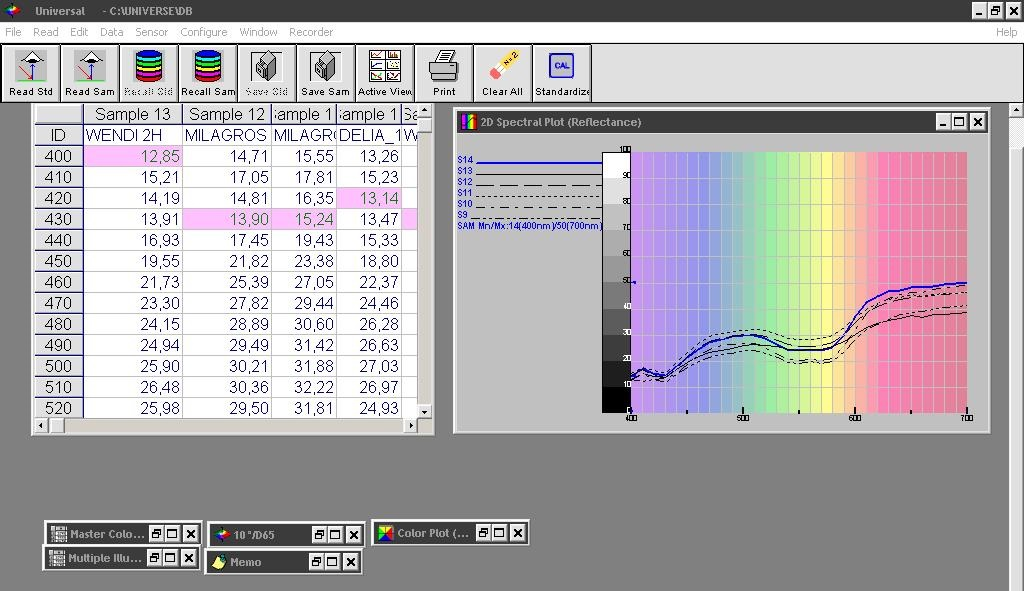
\includegraphics[scale=0.5]{img/universal.jpg}
			\caption[HunterLab Universal Software]{\textit{HunterLab Universal Software} (Fuente: CIMBUC, 2015).}
	\end{figure}

			El archivo denominado <<MSXE + OCX>>, es una hoja de c\'{a}lculo habilitada para la ejecuci\'{o}n de macroinstrucciones de Microsoft Excel, que fue proporcionada por el personal de soporte t\'{e}cnico de HunterLab como un ejemplo para utilizar el MiniScan XE Plus, empleando el uso de un kit de control denominado MiniScan XE Plus OCX Kit (MSXE.ocx). Este kit fue dise\~{n}ado por la empresa HunterLab para dar acceso a las caracter\'{i}sticas comunmente utilizadas por dicho instrumento. El c\'{o}digo contenido en la hoja de c\'{a}lculo se emple\'{o} como referencia para el manejo del kit MSXE.ocx.

	\section{Bases te\'{o}ricas}
	
	\subsection{Espectroscop\'{i}a de reflectancia difusa}
	
		La ERD es una t\'{e}cnica con la cual se puede estudiar tejido biol\'{o}gico. En el campo de las aplicaciones biom\'{e}dicas resulta \'{u}til para prop\'{o}sitos de diagn\'{o}stico, ya que se pueden estudiar tejidos de manera no invasiva, tambi\'{e}n ha demostrado ser una t\'{e}cnica de gran utilidad en aplicaciones de diagn\'{o}stico en varias situaciones modernas (P\'{e}rez, 2012).
		
		Para llevar a cabo una medici\'{o}n con ERD se requiere hacer incidir la luz de una fuente, cuyo espectro de emisi\'{o}n sea conocido, sobre el tejido que se quiere estudiar. La luz que logra propagarse en el tejido y que es re-emitida por \'{e}ste hacia la superficie irradiada, ser\'{a} capturada por alg\'{u}n dispositivo fotosensible (en el caso de esta investigaci\'{o}n, el MiniScan XE Plus), para ser comparada posteriormente con la luz incidente o espectro de referencia, y as\'{i} poder determinar qu\'{e} tanto cambi\'{o} dicho espectro despu\'{e}s de haber interactuado con el tejido.
		
		Normalmente los datos espectrales de la reflectancia difusa $R(\lambda)$ son multiplicados por un factor de 100 por los dispositivos fotosensibles, para representarlos en forma de curva en una escala del 0\% al 100\%, a lo largo de puntos discretos que representan las longitudes de onda con las que opera dicho dispositivo; tal es el caso del MiniScan XE Plus.
	
	\subsection{Absorbancia aparente}
	
	Seg\'{u}n el \textit{Random House Kernerman Webster's College Dictionary} (2010), el espectro de absorci\'{o}n es la radiaci\'{o}n electromagn\'{e}tica en ciertas longitudes de onda que atraviesa un medio, y que es absorbida por el mismo. En cierto modo, es el opuesto del espectro de reflectancia, es decir, es la luz que est\'{a} siendo absorbida aparentemente por el tejido en estudio, y que no est\'{a} siendo reflejada de vuelta al MiniScan XE Plus. Recordando que la reflectancia es multiplicada por un factor de 100 por el MiniScan XE Plus, la absorbancia se puede calcular con la ecuaci\'{o}n \ref{eq:absorbancia}.
	
\begin{equation}\label{eq:absorbancia}
	A(\lambda) = 100 - R(\lambda)
\end{equation}
	 
	 Los valores resultantes se pueden representar en forma de curva, de la misma manera que la reflectancia difusa.

	\subsection{Iluminante est\'{a}ndar D65}
		
		El tipo de luz bajo el cual se observa un objeto puede afectar su apariencia. Para cuantificar estas fuentes de luz blanca, la \textit{Commission Internationale de l'Eclairage} (CIE) desarroll\'{o} iluminantes est\'{a}ndares para la medici\'{o}n del color.
		\citeA{HunterLab} define el iluminante como una tabla cuantificable de n\'{u}meros que representan la energ\'{i}a relativa en comparaci\'{o}n con la longitud de onda de una fuente de luz. 
		
		El iluminante est\'{a}ndar D65, seg\'{u}n es descrito por la \citeA{CIE}, tiene el prop\'{o}sito de representar la luz de d\'{i}a promedio, y tiene una temperatura de color correlacionada de aproximadamente 6500 grados Kelvin. Los valores num\'{e}ricos que representan este iluminante se muestran en la tabla 2.1, y su representaci\'{o}n gr\'{a}fica se ilustra en la figura 2.2.
		
\newpage

		\begin{table}[h]
		\small
		\caption[Valores del iluminante D65]{\textit{Valores del iluminante D65} (Fuente: CIE, 2004).}
		\centering
		\setlength{\extrarowheight}{\altocelda}
		\begin{tabulary}{\anchotabla}{|c|c|}
			\hline
			Longitud de onda $\lambda$ & Funci\'{o}n $S(\lambda)$\\ \hline
			400 nm & 82.7549\\ \hline
			410 nm & 91.4860\\ \hline
			420 nm & 93.4318\\ \hline
			430 nm & 86.6823\\ \hline
			440 nm & 104.865\\ \hline
			450 nm & 117.008\\ \hline
			460 nm & 117.812\\ \hline
			470 nm & 114.861\\ \hline
			480 nm & 115.923\\ \hline
			490 nm & 108.811\\ \hline
			500 nm & 109.354\\ \hline
			510 nm & 107.802\\ \hline
			520 nm & 104.790\\ \hline
			530 nm & 107.689\\ \hline
			540 nm & 104.405\\ \hline
			550 nm & 104.046\\ \hline
			560 nm & 100.000\\ \hline
			570 nm & 96.3342\\ \hline
			580 nm & 95.7880\\ \hline
			590 nm & 88.6856\\ \hline
			600 nm & 90.0062\\ \hline
			610 nm & 89.5991\\ \hline
			620 nm & 87.6987\\ \hline
			630 nm & 83.2886\\ \hline
			640 nm & 83.6992\\ \hline
			650 nm & 80.0268\\ \hline
			660 nm & 80.2146\\ \hline
			670 nm & 82.2778\\ \hline
			680 nm & 78.2842\\ \hline
			690 nm & 69.7213\\ \hline
			700 nm & 71.6091\\ \hline
		\end{tabulary}
	\end{table}
	
\FloatBarrier

	\begin{figure}[H]
		\centering
		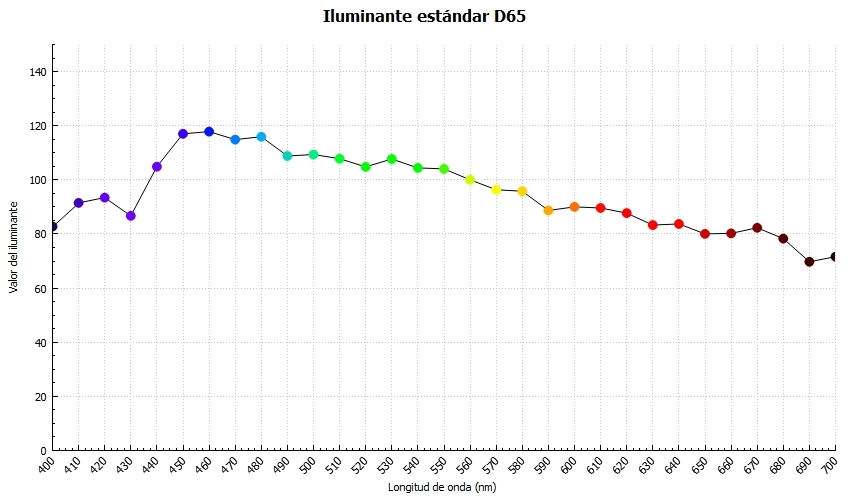
\includegraphics[scale=0.6]{img/curva-iluminante.jpg}
			\caption[Representaci\'{o}n gr\'{a}fica del iluminante est\'{a}ndar D65]{\textit{Representaci\'{o}n gr\'{a}fica del iluminante est\'{a}ndar D65} (Fuente: Autor).}
	\end{figure}

	\subsection{Observador est\'{a}ndar de 10 grados}
	
		\citeA{HunterLab-applications} describe que en la observaci\'{o}n visual, el observador es el ojo humano que recibe la luz reflejada desde o a trav\'{e}s de un objeto, y el cerebro el cual percibe la visi\'{o}n. Debido a que los humanos perciben el color y la apariencia de formas distintas, subjetivamente, se han hecho intentos para estandarizar el observador humano como una representaci\'{o}n de lo que una persona promedio ve u observa.
		
		En 1964, se desarroll\'{o} la funci\'{o}n del observador est\'{a}ndar CIE de 10 grados, denominado as\'{i} debido a que los experimentos llevados a cabo para establecer dicho est\'{a}ndar involucraron a sujetos que juzgaban colores, mientras observaban a trav\'{e}s de un agujero que les permit\'{i}a tener un campo de visi\'{o}n de 10 grados. Este observador est\'{a}ndar, en la forma de una funci\'{o}n matem\'{a}tica de la respuesta humana a cada longitud de onda de luz, es utilizado en c\'{a}lculos del color. Los valores num\'{e}ricos de las funciones que representan este est\'{a}ndar se muestran en la tabla 2.2, y su representaci\'{o}n gr\'{a}fica se ilustra en la figura 2.3.

\newpage

	\begin{table}[h]
		\small
		\caption[Valores del observador de 10 grados]{\textit{Valores del observador de 10 grados} (Fuente: CIE, 2004).}
		\centering
		\setlength{\extrarowheight}{\altocelda}
		\begin{tabulary}{\anchotabla}{|c|c|c|c|}
			\hline
			Longitud de onda $\lambda$ & Funci\'{o}n $\overline{x}(\lambda)$ & Funci\'{o}n $\overline{y}(\lambda)$ & Funci\'{o}n $\overline{z}(\lambda)$\\ \hline
			400 nm & 0.019110 & 0.002004 & 0.086011\\ \hline
			410 nm & 0.084736 & 0.008756 & 0.389366\\ \hline
			420 nm & 0.204492 & 0.021391 & 0.972542\\ \hline
			430 nm & 0.314679 & 0.038676 & 1.553480\\ \hline
			440 nm & 0.383734 & 0.062077 & 1.967280\\ \hline
			450 nm & 0.370702 & 0.089456 & 1.994800\\ \hline
			460 nm & 0.302273 & 0.128201 & 1.745370\\ \hline
			470 nm & 0.195618 & 0.185190 & 1.317560\\ \hline
			480 nm & 0.080507 & 0.253589 & 0.772125\\ \hline
			490 nm & 0.016172 & 0.339133 & 0.415254\\ \hline
			500 nm & 0.003816 & 0.460777 & 0.218502\\ \hline
			510 nm & 0.037465 & 0.606741 & 0.112044\\ \hline
			520 nm & 0.117749 & 0.761757 & 0.060709\\ \hline
			530 nm & 0.236491 & 0.875211 & 0.030451\\ \hline
			540 nm & 0.376772 & 0.961988 & 0.013676\\ \hline
			550 nm & 0.529826 & 0.991761 & 0.003988\\ \hline
			560 nm & 0.705224 & 0.997340 & 0.000000\\ \hline
			570 nm & 0.705224 & 0.955552 & 0.000000\\ \hline
			580 nm & 1.014160 & 0.868934 & 0.000000\\ \hline
			590 nm & 1.118520 & 0.777405 & 0.000000\\ \hline
			600 nm & 1.123990 & 0.658341 & 0.000000\\ \hline
			610 nm & 1.030480 & 0.527963 & 0.000000\\ \hline
			620 nm & 0.856297 & 0.398057 & 0.000000\\ \hline
			630 nm & 0.647467 & 0.283493 & 0.000000\\ \hline
			640 nm & 0.431567 & 0.179828 & 0.000000\\ \hline
			650 nm & 0.268329 & 0.107633 & 0.000000\\ \hline
			660 nm & 0.152568 & 0.060281 & 0.000000\\ \hline
			670 nm & 0.081261 & 0.031800 & 0.000000\\ \hline
			680 nm & 0.040851 & 0.015905 & 0.000000\\ \hline
			690 nm & 0.019941 & 0.007749 & 0.000000\\ \hline
			700 nm & 0.009577 & 0.003718 & 0.000000\\ \hline
		\end{tabulary}
		
	\end{table}
	
\FloatBarrier	
	
	\begin{figure}[H]
		\centering
		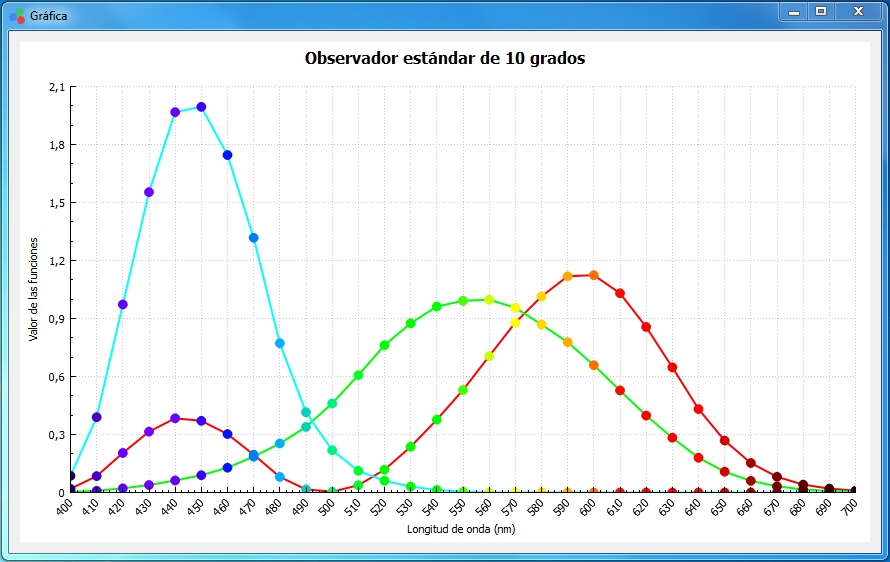
\includegraphics[scale=0.6]{img/curva-observador.jpg}
			\caption[Representaci\'{o}n gr\'{a}fica del observador de 10 grados]{\textit{Representaci\'{o}n gr\'{a}fica del observador de 10 grados. La l\'{i}nea roja representa la funci\'{o}n $\overline{x}(\lambda)$, la l\'{i}nea verde representa la funci\'{o}n $\overline{y}(\lambda)$, y la l\'{i}nea azul representa la funci\'{o}n $\overline{z}(\lambda)$.} (Fuente: Autor).}
	\end{figure}
	
	\subsection{Coordenadas de cromaticidad CIE xyz}
	
		La sensaci\'{o}n de luz es producida por radiaci\'{o}n electromagn\'{e}tica visible, que cae dentro de los l\'{i}mites de longitud de onda de 380 nan\'{o}metros y 780 nan\'{o}metros. La radiaci\'{o}n proveniente de la regi\'{o}n de longitud de onda corta produce usualmente la sensaci\'{o}n de luz azul, la radiaci\'{o}n con longitudes de onda entre 520 nan\'{o}metros y 550 nan\'{o}metros son vistas como luz verde, y por encima de los 650 nan\'{o}metros se percibe usualmente la luz de color rojo. Estos l\'{i}mites no est\'{a}n bien definidos, y la percepci\'{o}n actual depende fuertemente del estado de adaptaci\'{o}n del ojo y del est\'{i}mulo de luz que rodea el objeto en estudio (Schanda, 2007).
		
		La CIE defini\'{o} un est\'{a}ndar para calcular los valores de estos est\'{i}mulos, denominandolos valores triest\'{i}mulo CIE XYZ o sistema tricrom\'{a}tico CIE XYZ. Tomando en cuenta el rango de longitudes de onda con el que opera el \mbox{MiniScan} XE Plus, las f\'{o}rmulas para calcular estos valores se muestran en las ecuaciones \ref{eq:X}, \ref{eq:Y} y \ref{eq:Z}.
		
		\begin{equation}\label{eq:X}
			X = k \int_{400 \text{ nm}}^{700 \text{ nm}} R(\lambda) S(\lambda) \overline{x}(\lambda)d\lambda
		\end{equation}
		
		\begin{equation}\label{eq:Y}
			Y = k \int_{400 \text{ nm}}^{700 \text{ nm}} R(\lambda) S(\lambda) \overline{y}(\lambda)d\lambda
		\end{equation}
		
		\begin{equation}\label{eq:Z}
			Z = k \int_{400 \text{ nm}}^{700 \text{ nm}} R(\lambda) S(\lambda) \overline{z}(\lambda)d\lambda
		\end{equation}				
		
		En donde $R(\lambda)$ es el factor de reflectancia difusa, $S(\lambda)$ es la distribuci\'{o}n de energ\'{i}a espectral relativa de un iluminante est\'{a}ndar, en este caso del iluminante D65 (v\'{e}ase la tabla 2.1), $\overline{x}(\lambda)$, $\overline{y}(\lambda)$ y $\overline{z}(\lambda)$ son las funciones de correspondencia del color, dado el observador est\'{a}ndar CIE de 10 grados (v\'{e}ase la tabla 2.2), y por \'{u}ltimo, $k$ es una constante que se calcula con la f\'{o}rmula \ref{eq:k}.
		
		\begin{equation}\label{eq:k}
			k = \frac{100}{\sum_{\lambda} S(\lambda) \overline{y}(\lambda)d\lambda}
		\end{equation}
		
		De acuerdo con la recomendaci\'{o}n de la CIE, la integraci\'{o}n en las f\'{o}rmulas \ref{eq:X}, \ref{eq:Y} y \ref{eq:Z} puede llevarse a cabo con una sumatoria num\'{e}rica, con intervalos de longitud de onda equivalentes a 10 nan\'{o}metros para el caso del MiniScan XE Plus. Tomando en cuenta esto, los valores triest\'{i}mulo CIE XYZ se calculan con las ecuaciones \ref{eq:Xsum}, \ref{eq:Ysum} y \ref{eq:Zsum}.
		
		\begin{equation}\label{eq:Xsum}
			X = k \sum_{\lambda} R(\lambda) S(\lambda) \overline{x}(\lambda)\bigtriangleup\lambda
		\end{equation}
		
		\begin{equation}\label{eq:Ysum}
			Y = k \sum_{\lambda} R(\lambda) S(\lambda) \overline{y}(\lambda)\bigtriangleup\lambda
		\end{equation}
		
		\begin{equation}\label{eq:Zsum}
			Z = k \sum_{\lambda} R(\lambda) S(\lambda) \overline{z}(\lambda)\bigtriangleup\lambda
		\end{equation}
		
		Ahora bien, el est\'{i}mulo de un color se puede describir completamente por los tres valores triest\'{i}mulo, pero esta descripci\'{o}n no es concebible f\'{a}cilmente. Seg\'{u}n \citeA{Schanda}, es dif\'{i}cil imaginar un est\'{i}mulo si solamente se dan sus valores triest\'{i}mulo, y frecuentemente no se buscan los valores absolutos de los mismos. En tales casos se pueden utilizar las coordenadas de cromaticidad CIE xyz. Finalmente, dichas coordenadas se definen en las ecuaciones \ref{eq:x}, \ref{eq:y} y \ref{eq:z}.
		
		\begin{equation}\label{eq:x}
			x = \frac{X}{X+Y+Z}
		\end{equation}
		
		\begin{equation}\label{eq:y}
			y = \frac{Y}{X+Y+Z}
		\end{equation}
		
		\begin{equation}\label{eq:z}
			z = \frac{Z}{X+Y+Z}
		\end{equation}

	\subsection{Coordenadas del espacio CIELAB}
	
		Seg\'{u}n \citeA{Schanda}, los est\'{i}mulos del color son tridimensionales, y la solicitud de extender el espacio del color uniforme a un espacio tridimensional ya hab\'{i}a sido expresada en los a\~{n}os 60. En 1976 se acept\'{o} la recomendaci\'{o}n para el diagrama de espacio del color uniforme CIELAB (L*a*b*).
		
		El espacio del color CIELAB es un sistema para transformar las coordenadas de cromaticidad CIE xyz, a coordenadas L*a*b* representables en un espacio tridimensional, y est\'{a} definido por las ecuaciones \ref{eq:L}, \ref{eq:a} y \ref{eq:b}.
		
		\begin{equation}\label{eq:L}
			L^* = 116f(Y/Y_n) - 16
		\end{equation}
		
		\begin{equation}\label{eq:a}
			a^* = 500[f(X/X_n) - f(Y/Y_n)]
		\end{equation}
		
		\begin{equation}\label{eq:b}
			b^* = 200[f(Y/Y_n) - f(Z/Z_n)]
		\end{equation}
		
		$$\text{Donde } f(X/X_n) = (X/X_n)^{1/3} \text{ si } (X/X_n) > (24/116)^3$$
		$$f(X/X_n) = (841/108)(X/X_n) + 16/116 \text{ si } (X/X_n) \leq (24/116)^3$$
		
		$$\text{Donde } f(Y/Y_n) = (Y/Y_n)^{1/3} \text{ si } (Y/Y_n) > (24/116)^3$$
		$$f(Y/Y_n) = (841/108)(Y/Y_n) + 16/116 \text{ si } (Y/Y_n) \leq (24/116)^3$$
		
		$$\text{Donde } f(Z/Z_n) = (Z/Z_n)^{1/3} \text{ si } (Z/Z_n) > (24/116)^3$$
		$$f(Z/Z_n) = (841/108)(Z/Z_n) + 16/116 \text{ si } (Z/Z_n) \leq (24/116)^3$$
		
		En donde $X$, $Y$, $Z$ son los valores triest\'{i}mulo del color considerado del objeto o tejido en estudio y $X_n$, $Y_n$, $Z_n$ son los valores triest\'{i}mulo de la fuente de luz. Para el caso del iluminante est\'{a}ndar D65, y tomando en cuenta el observador est\'{a}ndar de 10 grados, los valores de $X_n$, $Y_n$, $Z_n$ son $X_n = 94.81$ $Y_n = 100.00$ y $Z_n = 107.32$.

	\subsection{Coeficiente de absorci\'{o}n}
	
		La piel es un medio biol\'{o}gico que se comporta perfectamente como un medio turbio multicapa, donde el principal agente de absorci\'{o}n es la melanina, la cual es producida en la epidermis, y es uno de los par\'{a}metros que determinan la coloraci\'{o}n de la piel \cite{Narea}.
		
		En la actualidad, existe el problema de calcular confiablemente los par\'{a}metros \'{o}pticos (entre ellos, el coeficiente de absorci\'{o}n) de los medios turbios a partir del conocimiento de su reflectancia. La determinaci\'{o}n de los par\'{a}metros \'{o}pticos es de vital importancia para el desarrollo de las investigaciones relativas a la caracterizaci\'{o}n de tejidos biol\'{o}gicos, en especial de la piel, empleando m\'{e}todos \'{o}pticos.
		
		\citeA{Narea} plantean recuperar el coeficiente de absorci\'{o}n de la epidermis a trav\'{e}s del ajuste trigonom\'{e}trico de los espectros de reflectancia difusa, brindando de esta forma una herramienta matem\'{a}tica que permite relacionar los par\'{a}metros del ajuste de las curvas espectrales con las propiedades \'{o}pticas de la piel.
		
		La f\'{o}rmula \ref{eq:absorcion} es la empleada para recuperar el coeficiente de absorci\'{o}n de la epidermis, dada una curva espectral $R(\lambda)$.
		
		\begin{equation}\label{eq:absorcion}
			\mu_{a,epi}(a_{0}, \lambda)=Ze^{ka_{0}}6,6 \cdot 10^{11}\lambda^{-3,3}
		\end{equation}
		
		En donde $Z=0,2796$, $k=-7,174$, y $a_{0}$ es un coeficiente hallado aplicando un ajuste polinomial por series trigonom\'{e}tricas a la curva espectral $R(\lambda)$.
	
	\subsection{\'{I}ndice de eritema}
	
		Una propiedad fundamental de la piel es su capacidad para responder a la radiaci\'{o}n ultravioleta. En muchas personas y poblaciones, estas respuestas son claramente adaptativas, en donde el eritema (enrojecimiento) es tanto una se\~{n}al para la persona quemada por el sol de buscar un resguardo, como una se\~{n}al de que el sistema inmunol\'{o}gico est\'{a} activo y el proceso de curaci\'{o}n ha comenzado \cite{Wagner}. 
		
		La respuesta de la piel result\'{o} ser importante cl\'{i}nicamente cuando los protocolos de tratamiento se establecieron en la d\'{e}cada de los 70 para reg\'{i}menes de fototerapia para la psoriasis y otras enfermedades de la piel. Para calcular el \'{i}ndice de eritema, primero hay que determinar el promedio ponderado de la reflectancia de la luz en el rango de longitud de onda verde, y en el rango de longitud de onda roja, utilizando las f\'{o}rmulas \ref{eq:Rverde} y \ref{eq:Rroja}.
		
		\begin{equation}\label{eq:Rverde}
			R_{verde} = \left.\left.\left[\left(\frac{1}{2}R_{560 \text{ nm}} + R_{570 \text{ nm}} + \frac{1}{2}R_{580 \text{ nm}}\right)\right/2\right]\right/100
		\end{equation}
		
		\begin{equation}\label{eq:Rroja}
			R_{roja} = \left.\left.\left[\left(\frac{1}{2}R_{640 \text{ nm}} + R_{650 \text{ nm}} + R_{660 \text{ nm}} + \frac{1}{2}R_{670 \text{ nm}}\right)\right/3\right]\right/100
		\end{equation}
		
		Teniendo ya el promedio ponderado de dichas reflectancias, la f\'{o}rmula \ref{eq:eritema} es la utilizada para calcular el \'{i}ndice de eritema.
		
		\begin{equation}\label{eq:eritema}
			E = 100 \cdot [\log(1/R_{verde}) - \log(1/R_{roja})]
		\end{equation}				
		
	\chapter{ Marco Metodol\'{o}gico}
	
	\section{Metodolog\'{i}a de investigaci\'{o}n}
	
		\subsection{Investigaci\'{o}n-Acci\'{o}n}
	\cite{Baskerville} define la Investigaci\'{o}n-Acci\'{o}n como un m\'{e}todo de investigaci\'{o}n que a finales de la d\'{e}cada de los 90 empez\'{o} a crecer en popularidad, para el uso en investigaciones acad\'{e}micas de sistemas de informaci\'{o}n. Este m\'{e}todo produce resultados de investigaci\'{o}n altamente relevantes debido a que se fundamenta en la acci\'{o}n pr\'{a}ctica, dirigida a resolver un problema mientras se informa cuidadosamente sobre la teor\'{i}a.

	Esta metodolog\'{i}a tiene una doble finalidad: generar un beneficio al cliente de la investigaci\'{o}n y al mismo tiempo generar conocimiento relevante. Por lo tanto, es una forma de investigar de car\'{a}cter colaborativo que busca unir teor\'{i}a y la pr\'{a}ctica entre investigadores y practicantes, mediante un proceso de naturaleza c\'{i}clica.

	La representaci\'{o}n m\'{a}s habitual de la Investigaci\'{o}n-Acci\'{o}n es la descrita por \cite{Baskerville}, en forma de cinco fases que conforman un ciclo, las cuales se muestran en la figura 3.1 y se describen a continuaci\'{o}n.

	\begin{figure}
		\centering
		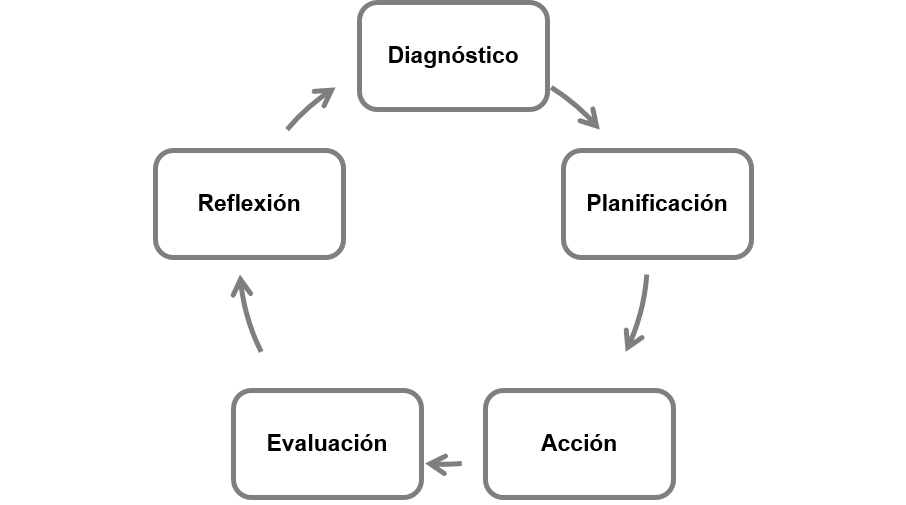
\includegraphics[scale=0.8]{img/investigacion-accion.png}
			\caption[Car\'{a}cter c\'{i}clico de la Investigaci\'{o}n-Acci\'{o}n]{\textit{Car\'{a}cter c\'{i}clico de la Investigaci\'{o}n-Acci\'{o}n} (Fuente: Baskerville, 1999).}
	\end{figure}

	\begin{itemize}
		\item \textbf{Fase de diagn\'{o}stico:} se realiza el proceso de identificaci\'{o}n de los problemas primarios de la investigaci\'{o}n.
		\item \textbf{Fase de planificaci\'{o}n:} se especifican las acciones que se llevar\'{a}n a cabo para solucionar los problemas primarios.
		\item \textbf{Fase de acci\'{o}n:} se ejecutan las acciones planificadas en la fase anterior.
		\item \textbf{Fase de evaluaci\'{o}n u observaci\'{o}n:} se efect\'{u}a una evaluaci\'{o}n de los resultados obtenidos para observar, conocer y documentar los efectos de las acciones que fueron realizadas.
		\item \textbf{Fase de reflexi\'{o}n:} se toman los conocimientos adquiridos en la Investigaci\'{o}n-Acci\'{o}n. Si las acciones ejecutadas no fueron exitosas, los conocimientos pueden proporcionar la base para el diagn\'{o}stico de un nuevo ciclo de Investigaci\'{o}n-Acci\'{o}n.
	\end{itemize}

En la tabla 3.1 se muestran las actividades de la presente investigaci\'{o}n, haciendo correspondencia a cada una de las fases de la Investigaci\'{o}n-Acci\'{o}n descritas por \cite{Baskerville}.

	\begin{table}[t]
		\small
		\caption[Actividades del proyecto seg\'{u}n la Investigaci\'{o}n-Acci\'{o}n]{\textit{Actividades del proyecto seg\'{u}n la Investigaci\'{o}n-Acci\'{o}n} (Fuente: Autor).}
		\centering
		\setlength{\extrarowheight}{\altocelda}
		\begin{tabulary}{\anchotabla}{|c|J|}
			\hline
			\thead{\textbf{\small{Fase}}} & \thead{\textbf{\small{Actividades}}}\\ \hline
			\textbf{Diagn\'{o}stico} & Identificar los problemas y limitaciones que presenta el HunterLab Universal Software.\\ \hline
			\textbf{Planificaci\'{o}n} & Seleccionar la metodolog\'{i}a de desarrollo, determinar los requisitos del software y realizar un plan de trabajo.
\\ \hline
			\textbf{Acci\'{o}n} & Desarrollar el software, tomando en cuenta los requisitos identificados previamente y los lineamientos de calidad del software.\\ \hline
			\textbf{Evaluaci\'{o}n} & Realizar las pruebas de funcionalidad y de usabilidad al software.\\ \hline
			\textbf{Reflexi\'{o}n} & Presentar los resultados y los an\'{a}lisis de las pruebas realizadas.\\ \hline
		\end{tabulary}
	\end{table}

\vspace*{0.5 cm}

	\section{Metodolog\'{i}a de desarrollo de software}
Para que el desarrollo del nuevo software cumpliera con los objetivos propuestos en la presente investigaci\'{o}n, y tomando en cuenta los atributos de calidad planteados por la ingenier\'{i}a del software, se realiz\'{o} una revisi\'{o}n del enfoque que deber\'{i}a tener la metodolog\'{i}a de desarrollo a utilizar.

Seg\'{u}n \cite{Sommerville}, en los a\~{n}os 80 y a principios de los 90, exist\'{i}a una opini\'{o}n general de que la mejor forma de obtener un software de calidad era a trav\'{e}s de una planificaci\'{o}n cuidadosa del proyecto, una garant\'{i}a de calidad formalizada, la utilizaci\'{o}n de m\'{e}todos de an\'{a}lisis y dise\~{n}o soportados por herramientas \textit{CASE}, y por medio de procesos de desarrollo de software controlados y rigurosos. El software que segu\'{i}a lo mencionado previamente era desarrollado por grandes equipos que a veces trabajaban para compa\~{n}\'{i}as diferentes, que a menudo estaban dispersos geogr\'{a}ficamente y trabajaban en el software durante largos periodos de tiempo.

Ahora bien, debido a que se ten\'{i}a un equipo peque\~{n}o para el desarrollo del nuevo software, y a que no se iba a trabajar en \'{e}ste durante un largo periodo de tiempo, se eligi\'{o} la utilizaci\'{o}n de una metodolog\'{i}a de desarrollo de enfoque \'{a}gil. De acuerdo con \cite{Sommerville}, los m\'{e}todos \'{a}giles dependen de un enfoque iterativo para la especificaci\'{o}n, el desarrollo y la entrega del software, y est\'{a}n pensados para entregar un producto funcional de forma r\'{a}pida a los clientes, quienes pueden entonces proponer que se incluyan en iteraciones posteriores nuevos requerimientos o cambios en los mismos. Si bien los m\'{e}todos \'{a}giles proponen procesos diferentes para el desarrollo y entregas incrementales del software, comparten unos principios en com\'{u}n, los cuales son ilustrados en la tabla 3.2.

	\begin{table}[t]
		\small
		\caption[Principios de los m\'{e}todos \'{a}giles]{\textit{Principios de los m\'{e}todos \'{a}giles} (Fuente: Sommerville, 2005).}
		\centering
		\setlength{\extrarowheight}{\altocelda}
		\begin{tabulary}{\anchotabla}{|c|J|}
			\hline
			\thead{\textbf{\small{Principio}}} & \thead{\textbf{\small{Descripci\'{o}n}}}\\ \hline
			\textbf{Participaci\'{o}n del cliente} & Los clientes deben estar fuertemente implicados en todo el proceso de desarrollo.\\ \hline
			\textbf{Entrega incremental} & El software se desarrolla en incrementos, en los que el cliente especifica los requerimientos a incluir en cada incremento.\\ \hline
			\textbf{Personas, no procesos} & Se deben reconocer y explotar las habilidades del equipo de desarrollo. A \'{e}ste se le debe dejar desarrollar su propia forma de trabajar, sin procesos formales.\\ \hline
			\textbf{Aceptar el cambio} & Se debe contar con que los requerimientos del software cambian, por lo que el software se dise\~{n}a para dar cabida a estos cambios.\\ \hline
			\textbf{Mantener la simplicidad} & Se debe centrar la simplicidad tanto en el software a desarrollar como en el proceso de desarrollo. Donde sea posible, se trabaja activamente para eliminar la complejidad del software.\\ \hline
		\end{tabulary}
	\end{table}

		\subsection{SCRUM}
De acuerdo con \cite{Schwaber&Sutherland}, esta metodolog\'{i}a \'{a}gil es un marco de trabajo de procesos, que ha sido utilizado para gestionar el desarrollo de productos complejos desde principios de los a\~{n}os 90. SCRUM muestra la eficacia relativa de las pr\'{a}cticas de gesti\'{o}n de productos y las pr\'{a}cticas de desarrollo.

La estructura de desarrollo de SCRUM se basa en ciclos de trabajo llamados \textit{sprints}. Los \textit{sprints} son iteraciones de una a cuatro semanas que suceden una detr\'{a}s de la otra, con una duraci\'{o}n fija y con fechas de culminaci\'{o}n previamente establecidas. Se seleccionan los requerimientos que se van a desarrollar de una lista priorizada. Todos los d\'{i}as el equipo se re\'{u}ne, y al final del \textit{sprint} el equipo revisa el mismo con los \textit{stakeholders}.

\cite{Hundermark} explica de forma precisa los roles que conforman el equipo de desarrollo de SCRUM, que se detallan a continuaci\'{o}n:
			
		\begin{itemize}
				
				\item \textbf{Due\~{n}o del producto \textit{(Product Owner)}:} su responsabilidad es optimizar el retorno de la inversi\'{o}n, asegurando que el equipo SCRUM este ocupado en entregar las caracter\'{i}sticas m\'{a}s valiosas del producto. Su trabajo principal es concentrarse en la efectividad, esto es elaborar el producto correcto para sus clientes.
				
				\item \textbf{Equipo de desarrollo:} es un grupo de personas responsables por entregar incrementos de la funcionalidad del producto al final de cada \textit{sprint}. El trabajo principal de este equipo es concentrarse en la eficiencia, esto es elaborar el producto correcto para su \textit{Product Owner} y sus usuarios.
				
				\item \textbf{Maestro SCRUM \textit{(SCRUM Master)}:} gestiona todos los aspectos del proceso del equipo SCRUM. Su trabajo principal es concentrarse en el progreso continuo del equipo, acortando los ciclos de retroalimentaci\'{o}n mediante los cuales aprende.
				
		\end{itemize}
			
			Como es sabido, el \textit{sprint} marca cada una de las iteraciones dentro del ciclo de desarrollo de SCRUM. Por otra parte, la planificaci\'{o}n, la continua revisi\'{o}n y la retrospectiva definen el inicio y el final del \textit{sprint}. Las reuniones que ocurren en cada \textit{sprint} son las siguientes.
			
			\begin{itemize}
				\item \textbf{Reuni\'{o}n de planificaci\'{o}n del \textit{sprint}: }
				esta reuni\'{o}n marca el inicio de cada \textit{sprint}. Su prop\'{o}sito para el equipo SCRUM es planear el trabajo que van a realizar durante el \textit{sprint} actual.
				
				\item \textbf{Reuni\'{o}n diaria del \textit{sprint}: }
				el equipo de desarrollo se reune para comunicar su trabajo, sincronizarlo y crear un plan para las siguientes 24 horas. Esta colaboraci\'{o}n es esencial para asegurar el progreso continuo y evadir cualquier obstrucci\'{o}n de trabajo.
				
				\item \textbf{Reuni\'{o}n de revisi\'{o}n del \textit{sprint}: }
				su prop\'{o}sito es el de inspeccionar la iteraci\'{o}n del producto que el equipo de desarrollo ha entregado, obtener una retroalimentaci\'{o}n de los participantes en la reuni\'{o}n con respecto a la misma, y adaptar el plan para el \textit{sprint} subsiguiente. Esta reuni\'{o}n est\'{a} abierta para todo el personal dentro de la organizaci\'{o}n.
				
				\item \textbf{Reuni\'{o}n de retrospectiva: }
				es la reuni\'{o}n final del \textit{sprint}, la cual nunca es omitida, sin importar lo que haya ocurrido en dicho \textit{sprint}. Mientras que la reuni\'{o}n de revisi\'{o}n del \textit{sprint} est\'{a} enfocada en el producto, esta reuni\'{o}n est\'{a} enfocada en el proceso, es decir, la forma en la que el equipo SCRUM est\'{a} trabajando en conjunto, incluyendo sus habilidades t\'{e}cnicas, las pr\'{a}cticas de desarrollo del software y las herramientas que est\'{a}n usando. Esta reuni\'{o}n se limita a los miembros del equipo SCRUM.
				
			\end{itemize}
			
Por otra parte, la metodolog\'{i}a SCRUM incluye los siguientes artefactos:
			
			\begin{itemize}
				\item \textbf{Pila del producto \textit{(product backlog)}: }
					es una lista de \'{i}tems de trabajo descritos en un nivel funcional, que necesitan ser realizados a lo largo del tiempo. Los requerimientos son emergentes, lo que significa que no se puede saber por adelantado todos los detalles acerca de lo que se quiere en el producto. Por esta raz\'{o}n este artefacto es un documento din\'{a}mico, que requiere un refinamiento constante para mantenerlo actual y \'{u}til.
				
				\item \textbf{Pila del \textit{sprint} \textit{(sprint backlog)}: }
				esta pila es visualizada por el equipo de desarrollo en un \textit{task board}, que es la representaci\'{o}n f\'{i}sica de la lista de trabajo que se ha resumido para realizar durante el \textit{sprint} actual. Este artefacto le dice al equipo SCRUM y a todos los dem\'{a}s el trabajo que tienen planeado hacer en el \textit{sprint}, y su estado actual.
				
				\item \textbf{Incremento: }
				es la suma de todos los \'{i}tems de la pila del producto que cumplen con la definici\'{o}n de terminado al final del \textit{sprint}. El equipo de desarrollo presentar\'{a} el incremento en la revisi\'{o}n del \textit{sprint}, y el \textit{Product Owner} determinar\'{a} cu\'{a}ndo liberarlo.
				
			\end{itemize}
			
En esta metodolog\'{i}a se pueden emplear varias t\'{e}cnicas y procesos. En este sentido, se incluyeron algunos artefactos de la metodolog\'{i}a RUP (\textit{Rational Unified Process}) descrita por \cite{Kroll&Kruchten}, para as\'{i} generar suficiente documentaci\'{o}n durante el dise\~{n}o y el desarrollo del software. 

	\subsection{Artefactos de RUP utilizados}
	
		\begin{itemize}
			\item \textbf{Documento de visi\'{o}n: }describe la visi\'{o}n de los \textit{stakeholders} con respecto al producto a desarrollarse, especificado en t\'{e}rminos de las caracter\'{i}sticas y las necesidades claves de los mismos.
			
			\item \textbf{Modelo de casos de uso: }describe los requerimientos funcionales del software en t\'{e}rminos de actores y casos de uso. Un actor representa el tipo de usuario del software, mientras que un caso de uso describe c\'{o}mo va a interactuar cada actor con el software.
			
			\item \textbf{Requerimientos no funcionales: } representan los requerimientos que tienen un impacto significativo en la arquitectura y en la satisfacci\'{o}n del usuario.
			
			\item \textbf{Glosario: }define la terminolog\'{i}a empleada en todos los artefactos utilizados.
		\end{itemize}

\newpage

Para finalizar, en la figura 3.2 se ilustra la configuraci\'{o}n de la metodolog\'{i}a SCRUM utlizada, en conjunto con los artefactos elegidos de la metodolog\'{i}a RUP.
	
	\FloatBarrier
	\begin{figure}[h]
		\centering
		
\includegraphics[scale=0.8]{img/SCRUM-RUP.png}
			\caption[Configuraci\'{o}n de los artefactos a utilizar de SCRUM y RUP]{\textit{Configuraci\'{o}n de los artefactos a utilizar de SCRUM y RUP} (Fuente: Autor).}
	\end{figure}
	\FloatBarrier
	
	\chapter{ Resultados}

\section{Fases metodol\'{o}gicas}

\subsection{Visi\'{o}n}
	
	\subsubsection{Enunciado del problema}
	
	El problema que se presenta es que se est\'{a} utilizando el HunterLab Universal Software para el manejo del espectrofot\'{o}metro de reflexi\'{o}n difusa MiniScan XE Plus. Dicho software est\'{a} en ingl\'{e}s, es comercial, privativo y fue descontinuado; esto afecta a los dermat\'{o}logos del CIMBUC.
	
	El impacto causado por esto es que los dermat\'{o}logos encuentran el HunterLab Universal Software dif\'{i}cil de utilizar e imposible de adaptar a sus necesidades, lo que ralentiza la actividad de consulta con sus pacientes, genera la necesidad de disponer de personal especializado para su debido uso y disminuye el potencial de dicho instrumento.
	
	Una soluci\'{o}n satisfactoria ser\'{i}a disponer de un software para el uso del \mbox{MiniScan} XE Plus que est\'{e} en espa\~{n}ol, que sea amigable y mantenible, permitiendo que se adapte a las necesidades de los dermat\'{o}logos.
	
	\subsubsection{Descripci\'{o}n de los usuarios}
	
		\begin{table}[h]
		\small
		\caption[Actores del negocio]{\textit{Actores del negocio} (Fuente: Autor).}
		\centering
		\setlength{\extrarowheight}{\altocelda}
		\begin{tabulary}{\anchotabla}{|c|J|}
			\hline
			\thead{\textbf{\small{Actor}}} & \thead{\textbf{\small{Descripci\'{o}n}}}\\ \hline
			\textbf{Administrador} &
			
			Realiza mediciones.
			
			Consulta las historias m\'{e}dicas de los pacientes y las muestras.
			
			Gestiona los usuarios.
		\\ \hline
			\textbf{Dermat\'{o}logo} &
			
			Realiza mediciones.
			
			Gestiona las historias m\'{e}dicas de los pacientes y las muestras.
			
			Realiza diagn\'{o}sticos a partir de los resultados de las muestras.
		\\ \hline
			\textbf{Investigador} &
			
			Realiza mediciones.
			
			Consulta las historias m\'{e}dicas de los pacientes y las muestras.
			
			Realiza an\'{a}lisis sobre los resultados de las mediciones.\\ \hline
		\end{tabulary}
	\end{table}
	
	\begin{table}[h]
		\small
		\caption[Actores del software]{\textit{Actores del software} (Fuente: Autor).}
		\centering
		\setlength{\extrarowheight}{\altocelda}
		\begin{tabulary}{\anchotabla}{|c|J|c|c|}
			\hline
			\thead{\textbf{\small{Actor}}} & \thead{\textbf{\small{Responsabilidad}}} & \thead{\textbf{\small{Experiencia}}} & \thead{\textbf{\small{Uso}}}\\ \hline
			
			\textbf{Administrador} &
			
			Manejar el MiniScan XE Plus.
			
			Crear, consultar, modificar y eliminar usuarios.
			
			Consultar historias m\'{e}dicas de pacientes.
			
			Consultar muestras de pacientes. &
			Alta &
			Alto\\ \hline
			
			\textbf{Dermat\'{o}logo} &
			
			Manejar el MiniScan XE Plus.
			
			Crear, consultar, modificar y eliminar historias m\'{e}dicas de pacientes.
			
			Crear, consultar, modificar y eliminar muestras de pacientes. &
			Baja &
			Alto\\ \hline
			
			\textbf{Investigador} &
			
			Manejar el MiniScan XE Plus.
			
			Consultar historias m\'{e}dicas de pacientes.
			
			Consultar muestras de pacientes. &
			Media &
			Alto\\ \hline
		\end{tabulary}
	\end{table}
	
	\subsubsection{Resumen del producto}
	
	El software desarrollado, denominado a partir de ahora Spectrasoft, es una aplicaci\'{o}n para el uso del MiniScan XE Plus, destinado a la recuperaci\'{o}n de los datos de medici\'{o}n de dicho instrumento, y a la generaci\'{o}n y gesti\'{o}n de resultados relevantes. Dicho software estar\'{a} orientado a las actividades m\'{e}dicas dermatol\'{o}gicas del CIMBUC. La tabla 4.3 resume los beneficios y las caracter\'{i}sticas m\'{a}s importantes que provee el producto.
	
	\begin{table}[h]
		\small
		\caption[Beneficios y caracter\'{i}sticas principales del producto]{\textit{Beneficios y caracter\'{i}sticas principales del producto} (Fuente: Autor).}
		\centering
		\setlength{\extrarowheight}{\altocelda}
		\begin{tabulary}{\anchotabla}{|J|J|}
			\hline
			\thead{\textbf{\small{Beneficio al cliente}}} & \thead{\textbf{\small{Caracter\'{i}stica que lo soporta}}}\\ \hline
			Se puede conectar, calibrar y realizar mediciones con el MiniScan XE Plus. & 
			Comunicaci\'{o}n con el MiniScan XE Plus y acceso a las caracter\'{i}sticas comunmente utilizadas por el mismo.\\ \hline
			Se dispone de informaci\'{o}n relevante para el an\'{a}lisis y diagn\'{o}stico de patolog\'{i}as dermatol\'{o}gicas en la piel de los pacientes. &
			Muestra de los datos espectrales obtenidos de las mediciones, representaci\'{o}n gr\'{a}fica de dichos datos, y c\'{a}lculo de valores adicionales asociados a los mismos.\\ \hline
			Se pueden gestionar los usuarios, las historias m\'{e}dicas y las muestras generadas de las mediciones. &
			Manejo de una base de datos que almacena toda la informaci\'{o}n referente a los usuarios, las historias m\'{e}dicas y las muestras, permitiendo su gesti\'{o}n por medio del Spectrasoft.\\ \hline
			El Spectrasoft se puede utilizar con facilidad. &
			Interfaz gr\'{a}fica de usuario en espa\~{n}ol, que ofrece \'{u}nicamente las funciones necesarias para gestionar la informaci\'{o}n que necesitan los usuarios. \\ \hline
			El Spectrasoft se puede adaptar a las futuras necesidades de sus usuarios. &
			C\'{o}digo abierto del proyecto disponible en su totalidad para realizar cualquier modificaci\'{o}n y/o extensi\'{o}n.\\ \hline
		\end{tabulary}
	\end{table}
	
	\subsubsection{Principales restricciones}
	
	El software se desarrolla utilizando el lenguaje de programaci\'{o}n C++, empleando \'{u}nicamente tecnolog\'{i}as gratuitas, y en la medida de lo posible, de c\'{o}digo abierto. Se ejecuta en sistemas operativos Windows actuales. Por \'{u}ltimo, la comunicaci\'{o}n entre el software y el MiniScan XE Plus se logra por medio de un puerto serial, o a trav\'{e}s de un adaptador USB.
	
\subsection{Pila del producto \textit{(product backlog)}}
	La lista de requerimientos funcionales que necesitan ser realizados a lo largo del desarrollo del Spectrasoft son el producto de una reuni\'{o}n que se tuvo con los dermat\'{o}logos y los investigadores del CIMBUC, al igual que de la observaci\'{o}n directa efectuada a las funciones que el HunterLab Universal Software ofrece para el manejo del MiniScan XE Plus. En la tabla 4.4 se muestran dichos requerimientos.
	
	\begin{table}[h]
		\small
		\caption[Requerimientos funcionales del software]{\textit{Requerimientos funcionales del software} (Fuente: Autor).}
		\centering
		\setlength{\extrarowheight}{\altocelda}
		\begin{tabulary}{\anchotabla}{|c|J|c|}
			\hline
			\thead{\textbf{\small{C\'{o}digo}}} & \thead{\textbf{\small{Requerimiento}}} & \thead{\textbf{\small{Prioridad}}}\\ \hline
			
			\textbf{RF01} & Conectar y desconectar el MiniScan XE Plus. & Esencial\\ \hline
			
			\textbf{RF02} & Calibrar el MiniScan XE Plus. & Esencial\\ \hline
			
			\textbf{RF03} & Recuperar los 31 puntos espectrales de una medici\'{o}n con el MiniScan XE Plus y mostrarlos en su forma num\'{e}rica. & Esencial\\ \hline

			\textbf{RF04} & Graficar una curva de reflectancia difusa a partir de los 31 puntos espectrales recuperados. & Esencial\\ \hline
			\textbf{RF05} & Graficar una curva de absorbancia aparente a partir de los 31 puntos espectrales recuperados. & Esencial\\ \hline
			\textbf{RF06} & Calcular y mostrar las coordenadas de cromaticidad CIE xyz. & Esencial\\ \hline
			
			\textbf{RF07} & Calcular y mostrar las coordenadas del espacio CIELAB. & Esencial\\ \hline

			\textbf{RF08} & Calcular y graficar el coeficiente de absorci\'{o}n de la epidermis. & Esencial\\ \hline

			\textbf{RF09} & Calcular y mostrar el \'{i}ndice de eritema. & Esencial\\ \hline

			\textbf{RF10} & Almacenar la informaci\'{o}n de los usuarios, las historias m\'{e}dicas, las muestras y los resultados de las mediciones en una base de datos. & Esencial\\ \hline			

			\textbf{RF11} & Gestionar la creaci\'{o}n, consulta, modificaci\'{o}n y eliminaci\'{o}n de los usuarios. & Esencial\\ \hline
			
			\textbf{RF12} & Gestionar la creaci\'{o}n, consulta, modificaci\'{o}n y eliminaci\'{o}n de las historias m\'{e}dicas de pacientes. & Esencial\\ \hline
			
			\textbf{RF13} & Gestionar la creaci\'{o}n, consulta, modificaci\'{o}n y eliminaci\'{o}n de las muestras pertenecientes a las historias m\'{e}dicas. & Esencial\\ \hline	
			
			\textbf{RF14} & Exportar los datos de una muestra a un archivo port\'{a}til. & Esencial\\ \hline
		\end{tabulary}
	\end{table}
	
\subsection{Requerimientos no funcionales}
	
	De la misma forma que los requerimientos funcionales, la lista de los requerimientos no funcionales fue definida en la misma reuni\'{o}n con los dermat\'{o}logos y los investigadores, tomando en cuenta las restricciones del entorno en donde se va a ejecutar el Spectrasoft. En la tabla 4.5 se describen estos requerimientos no funcionales.
	
	\begin{table}[h]
		\small
		\caption[Requerimientos no funcionales del software]{\textit{Requerimientos no funcionales del software} (Fuente: Autor).}
		\centering
		\setlength{\extrarowheight}{\altocelda}
		\begin{tabulary}{\anchotabla}{|c|J|c|}
			\hline
			\thead{\textbf{\small{C\'{o}digo}}} & \thead{\textbf{\small{Requerimiento}}} & \thead{\textbf{\small{Prioridad}}}\\ \hline
			\textbf{RNF01} & El software debe ser f\'{a}cil de utilizar, por lo que debe cumplir con el atributo de usabilidad de un software de calidad. & Esencial\\ \hline
			\textbf{RNF02} & El software debe ser capaz de adaptarse a las necesidades de los dermat\'{o}logos, permitiendo la incorporaci\'{o}n de nuevos requerimientos y funcionalidades, raz\'{o}n por la cual debe cumplir con el atributo de mantenibilidad de un software de calidad. & Esencial\\ \hline
			\textbf{RNF03} & El software debe desarrollarse empleando \'{u}nicamente herramientas y tecnolog\'{i}as gratuitas, y en la medida de lo posible, libres. & Esencial\\ \hline
			\textbf{RNF04} & El software debe ser capaz de ejecutarse en sistemas Windows actuales, con arquitecturas de 32 bits y 64 bits. & Esencial\\ \hline
			\textbf{RNF05} & El software debe conectarse con el MiniScan XE Plus por medio de un puerto serial o de un adaptador USB. & Esencial\\ \hline
			\textbf{RNF06} & El archivo port\'{a}til al que se exportan los resultados de una medici\'{o}n debe ser abierto por un visualizador/editor de hojas de c\'{a}lculo. & Esencial\\ \hline
			\textbf{RNF07} & El software debe desarrollarse utilizando el lenguaje de programaci\'{o}n orientada a objetos C++. & Esencial\\ \hline
		\end{tabulary}
	\end{table}
	
\newpage

\subsection{Casos de uso}

 \begin{itemize}
 	
 	\item \textbf{Operar el MiniScan XE Plus:}
 	
 		\begin{figure}[H]
		\centering
		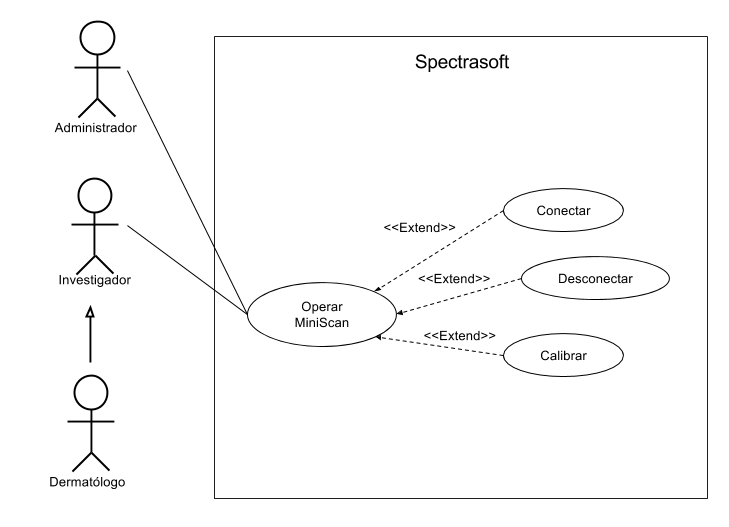
\includegraphics[scale=0.4]{img/cu-manejar-miniscan.png}
			\caption[Caso de uso: operar el MiniScan XE Plus]{\textit{Caso de uso: operar el MiniScan XE Plus} (Fuente: Autor).}
	\end{figure}
	
	 	\item \textbf{Gestionar medici\'{o}n:}
 	
 		\begin{figure}[H]
		\centering
		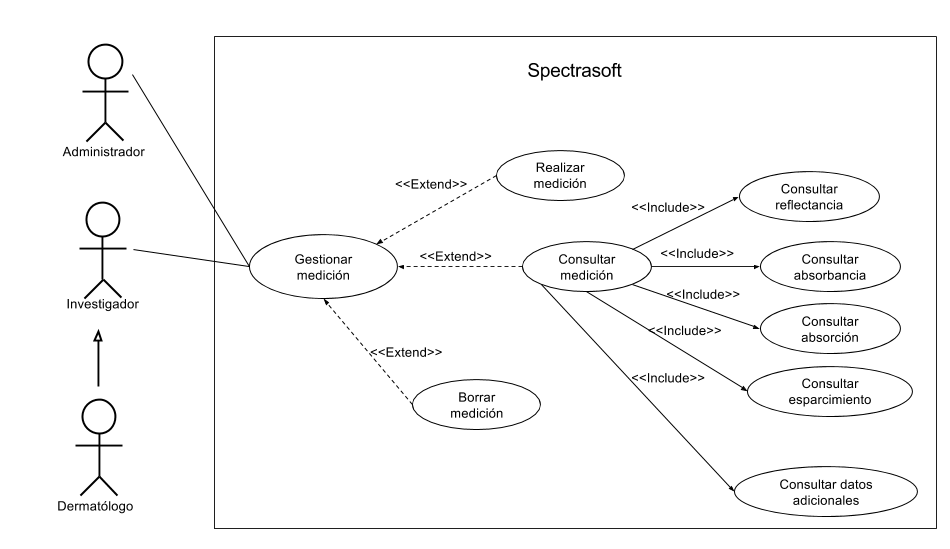
\includegraphics[scale=0.4]{img/cu-gestion-medicion.png}
			\caption[Caso de uso: gestionar medici\'{o}n]{\textit{Caso de uso: gestionar medici\'{o}n} (Fuente: Autor).}
	\end{figure}

\newpage
	 	\item \textbf{Gestionar sesi\'{o}n de usuario:}
 	
 		\begin{figure}[H]
		\centering
		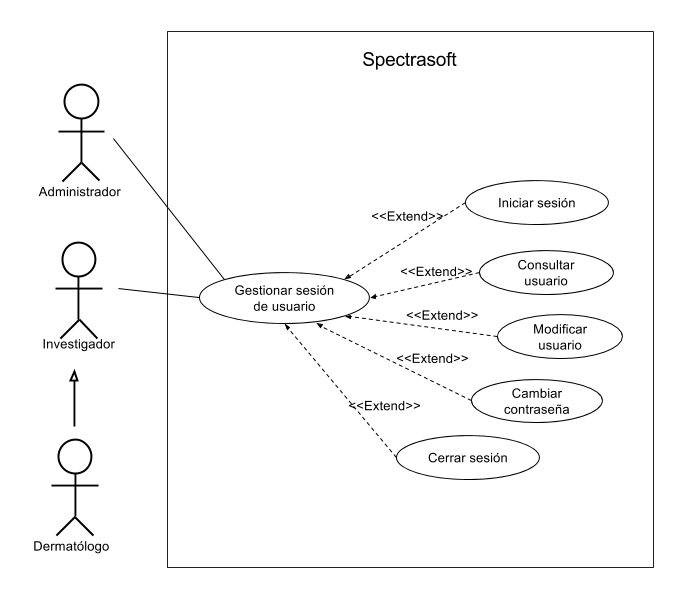
\includegraphics[scale=0.5]{img/cu-gestion-sesion.png}
			\caption[Caso de uso: gestionar sesi\'{o}n de usuario]{\textit{Caso de uso: gestionar sesi\'{o}n de usuario} (Fuente: Autor).}
	\end{figure}
	
		 	\item \textbf{Gestionar historia:}
 	
 		\begin{figure}[H]
		\centering
		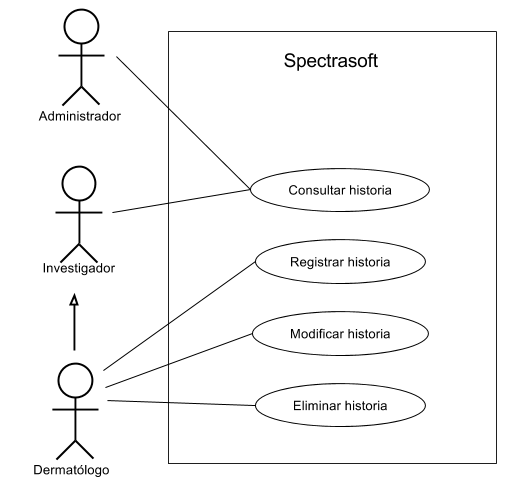
\includegraphics[scale=0.5]{img/cu-gestion-historia.png}
			\caption[Caso de uso: gestionar historia]{\textit{Caso de uso: gestionar historia} (Fuente: Autor).}
	\end{figure}

\newpage
		\item \textbf{Gestionar muestra:}
 	
 		\begin{figure}[H]
		\centering
		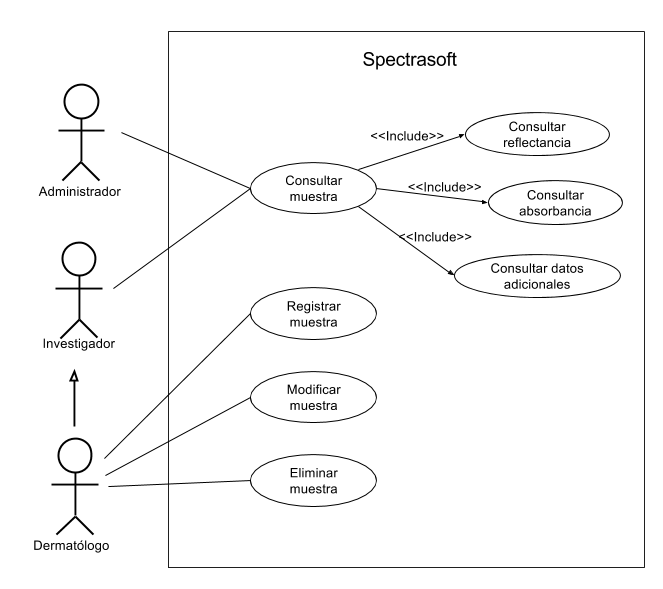
\includegraphics[scale=0.5]{img/cu-gestion-muestra.png}
			\caption[Caso de uso: gestionar muestra]{\textit{Caso de uso: gestionar muestra} (Fuente: Autor).}
	\end{figure}
	
		\item \textbf{Gestionar usuario:}
 	
 		\begin{figure}[H]
		\centering
		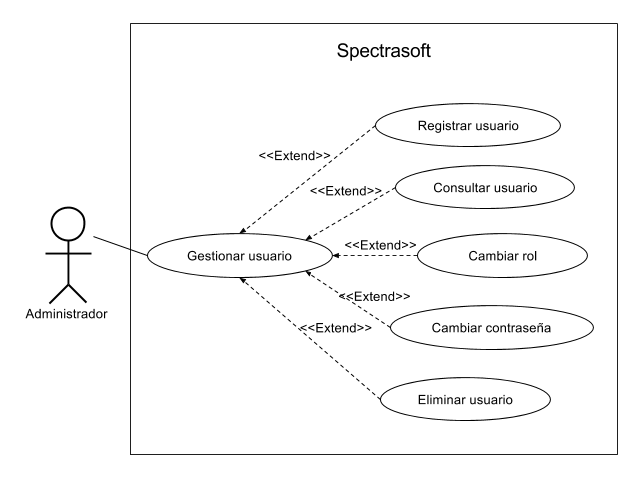
\includegraphics[scale=0.5]{img/cu-gestion-usuario2.png}
			\caption[Caso de uso: gestionar usuario]{\textit{Caso de uso: gestionar usuario} (Fuente: Autor).}
		\end{figure}
			
		\item \textbf{Caso de uso general:}
 	
 		\begin{figure}[H]
		\centering
		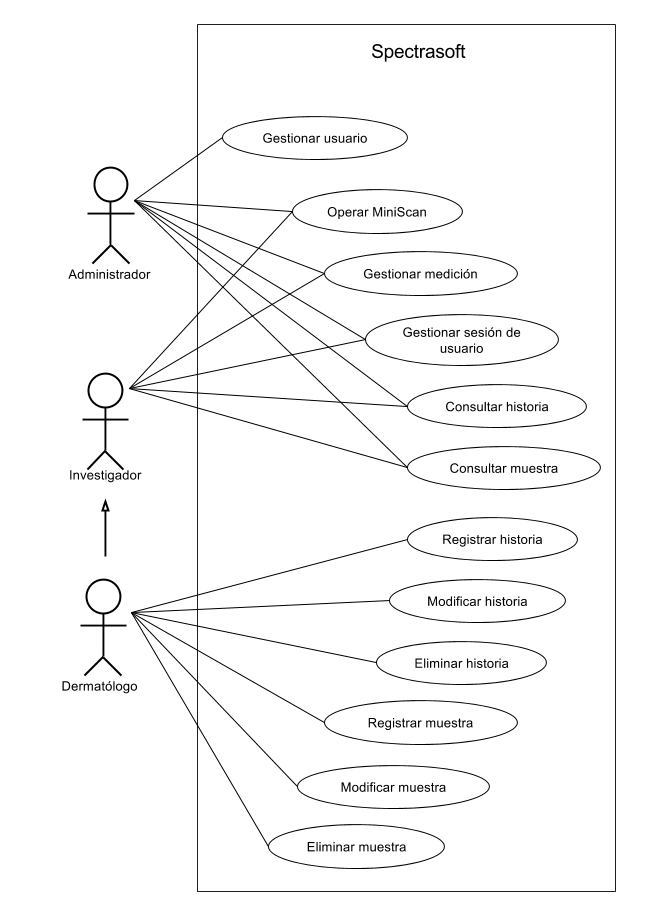
\includegraphics[scale=0.6]{img/cu-general.png}
			\caption[Caso de uso general]{\textit{Caso de uso general} (Fuente: Autor).}
		\end{figure}
	
 \end{itemize}
 
\newpage
 
	\subsubsection{Descripci\'{o}n de los casos de uso}
	
		\begin{itemize}
			\item \textbf{Operar MiniScan:} Permite a todos los usuarios conectar, desconectar y calibrar el MiniScan XE Plus, esto \'{u}ltimo haciendo uso de una trampa de luz y una cer\'{a}mica blanca.
			
			\item \textbf{Gestionar medici\'{o}n:} Permite a todos los usuarios efectuar una medici\'{o}n con el MiniScan XE Plus conectado, visualizar los resultados obtenidos de la misma, y borrarlos.
			
			\item \textbf{Consultar medici\'{o}n:} Permite a todos los usuarios visualizar tanto la informaci\'{o}n obtenida directamente del MiniScan XE Plus, como la informaci\'{o}n calculada a partir de la misma, como la curva de reflectancia difusa, la curva de absorbancia aparente, las coordenadas de cromaticidad CIE xyz, las coordenadas CIELAB, el coeficiente de absorci\'{o}n y el \'{i}ndice de eritema de una medici\'{o}n realizada.
			
			\item \textbf{Gestionar sesi\'{o}n de usuario:} Permite a cualquier usuario iniciar sesi\'{o}n para acceder a las funciones pertinentes a su rol, consultar y modificar su informaci\'{o}n, cambiar su contrase\~{n}a, y cerrar sesi\'{o}n.
			
			\item \textbf{Gestionar historia:} Permite a todos los usuarios consultar la informaci\'{o}n perteneciente a las historias m\'{e}dicas, y s\'{o}lo permite a los usuarios con el rol de dermat\'{o}logo registrar, modificar y eliminar dichas historias. 
			
			\item \textbf{Gestionar muestra:} Permite a todos los usuarios consultar la informaci\'{o}n referente a las muestras pertenecientes a una historia m\'{e}dica de un paciente determinado, as\'{i} como exportar dicha informaci\'{o}n, y s\'{o}lo permite a los usuarios con el rol de dermat\'{o}logo registrar, modificar y eliminar tales muestras.
			
			\item \textbf{Gestionar usuario:} Permite registrar usuarios, consultar su informaci\'{o}n, cambiar los roles de dichos usuarios, cambiar sus contrase\~{n}as y eliminarlos. Esto solamente puede ser efectuado por usuarios con el rol de administrador.
		\end{itemize}

\subsection{Glosario}

\begin{itemize}
	
	\item \textbf{Espectroscop\'{i}a de reflectancia difusa:}  t\'{e}cnica con la cual se puede estudiar tejido biol\'{o}gico.

	\item \textbf{Espectrofot\'{o}metro de reflexi\'{o}n difusa:} instrumento de medici\'{o}n del color, que emplea la t\'{e}cnica de espectroscop\'{i}a de reflectancia difusa.
	
	\item \textbf{Medici\'{o}n:} es un proceso b\'{a}sico de la ciencia que consiste en comparar un patr\'{o}n seleccionado con el objeto o fen\'{o}meno cuya magnitud f\'{i}sica se desea medir, para ver cu\'{a}ntas veces el patr\'{o}n est\'{a} contenido en esa magnitud.
	
	\item \textbf{Calibraci\'{o}n:} proceso de comparar los valores obtenidos por un instrumento de medici\'{o}n con la medida correspondiente de un patr\'{o}n de referencia.
	
	\item \textbf{Historia m\'{e}dica:} documento m\'{e}dico-legal que surge del contacto entre el profesional de la salud (en este caso, dermat\'{o}logo) y el paciente, donde se recoge la informaci\'{o}n necesaria para la correcta atenci\'{o}n de los pacientes.
	
	\item \textbf{Muestra:} parte o cantidad peque\~{n}a de una cosa que se considera representativa del total y que se toma o se separa de ella con ciertos m\'{e}todos para someterla a estudio, an\'{a}lisis o experimentaci\'{o}n.
	
	\item \textbf{Patolog\'{i}a dermatol\'{o}gica:} parte de la medicina dermatol\'{o}gica que estudia los trastornos anat\'{o}micos y fisiol\'{o}gicos de la piel, as\'{i} como los s\'{i}ntomas y signos a trav\'{e}s de los cuales se manifiestan las enfermedades y las causas que las producen.
	
	\item \textbf{Datos espectrales:} datos que representan un conjunto de ondas electromagn\'{e}ticas, ordenadas seg\'{u}n su frecuencia.
	
	\item \textbf{Absorbancia aparente:} es la luz que aparentemente est\'{a} siendo absorbida por un medio.
	
	\item \textbf{Coordenadas de cromaticidad CIE xyz:} valores que representan los est\'{i}mulos de la luz de una forma est\'{a}ndar.
	
	\item \textbf{Coordenadas del espacio CIELAB:} valores obtenidos de la transformaci\'{o}n de las coordenadas de cromaticidad CIE xyz, haciendolas representables en un espacio de tres dimensiones.
	
	\item \textbf{Epidermis:} membrana epitelial que recubre la parte m\'{a}s superficial del cuerpo de los animales.	
	
	\item \textbf{Coeficiente de absorci\'{o}n:} conjunto de valores que indican el nivel de concentraci\'{o}n de melanina presente en la epidermis de un paciente.
	
	\item \textbf{\'{I}ndice de eritema:} valor utilizado para determinar el nivel inflamatorio de la epidermis de un paciente.
	
\end{itemize}

\newpage

\section{Base de datos}

	\subsection{Diagrama ER de la base de datos}

	\begin{figure}[H]
		\centering
		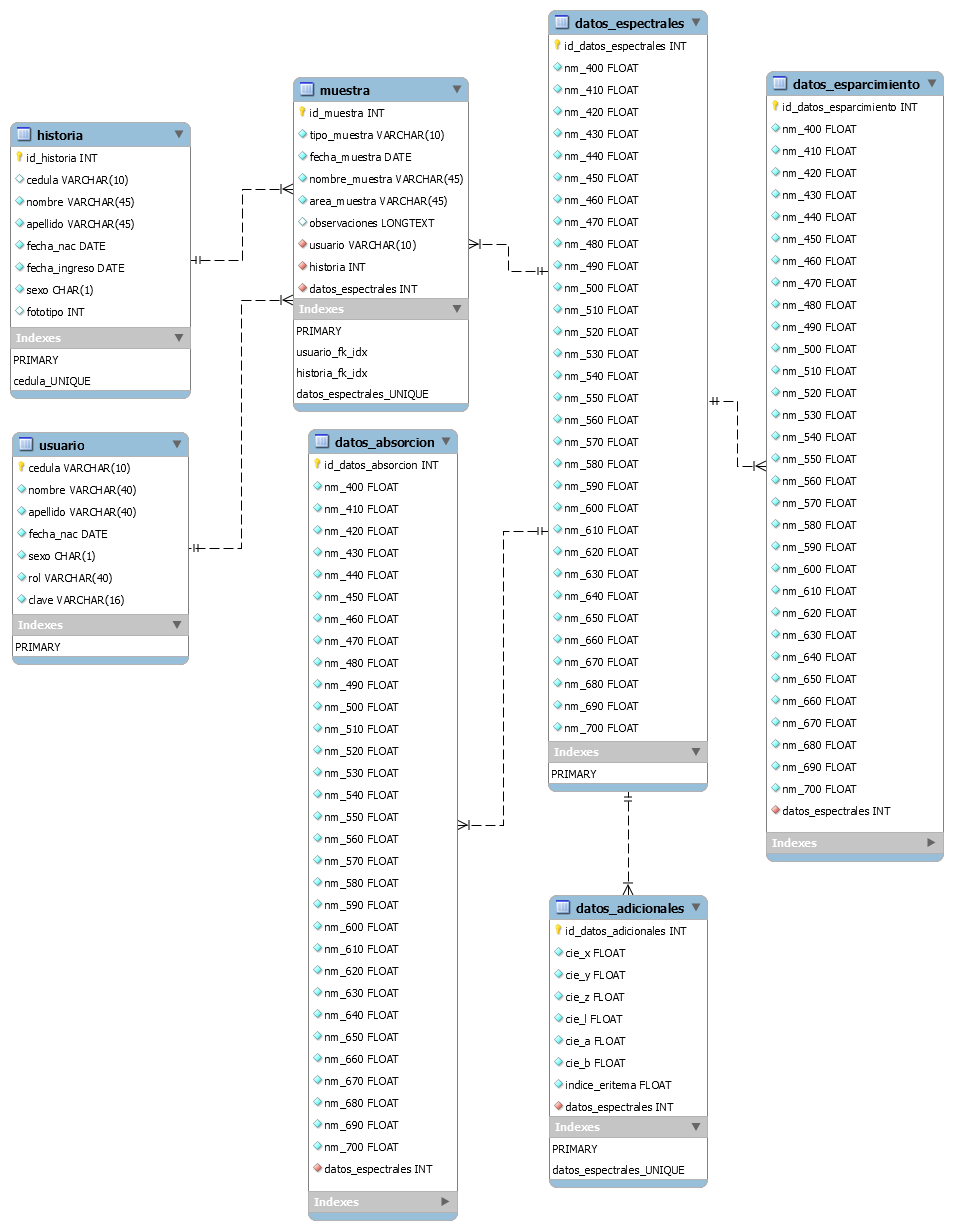
\includegraphics[scale=.4]{img/diagramaER.png}
			\caption[Diagrama ER de la base de datos]{\textit{Diagrama ER de la base de datos} (Fuente: Autor).}
	\end{figure}
	
	\subsection{Descripci\'{o}n de las tablas de la base de datos}
	
		\begin{itemize}
				
				\item \textbf{historia:} almacena los datos referentes a la historia m\'{e}dica de cada uno de los pacientes registrados.
				
				\item \textbf{usuario:} guarda la informaci\'{o}n de cada uno de los usuarios que pueden acceder al software, que pueden ser administradores, dermat\'{o}logos o investigadores.
				
				\item \textbf{muestra:} contiene los datos relevantes de las muestras que son tomadas a los pacientes. Dichas muestras siempre est\'{a}n interrelacionadas con la historia m\'{e}dica del paciente al que pertenece, y la c\'{e}dula del usuario que la tom\'{o}.

				\item \textbf{datos\_espectrales:} contiene los 31 puntos espectrales resultantes de la medici\'{o}n realizada sobre cada muestra por medio del MiniScan XE Plus.
				
				\item \textbf{datos\_absorcion:} contiene los 31 puntos espectrales resultantes del c\'{a}lculo del coeficiente de absorci\'{o}n asociado con los datos espectrales.
				
				\item \textbf{datos\_adicionales:} almacena los datos que son calculados a partir de los 31 puntos espectrales de cada muestra, estos son las coordenadas de cromaticiad CIE xyz, las coordenadas del espacio del color CIELAB y el \'{i}ndice de eritema.
				
		\end{itemize}

\section{Tecnolog\'{i}as y recursos utilizados}

	\subsection{Tecnolog\'{i}as}
	
		\begin{itemize}
			
			\item \textbf{Qt:} es un \textit{framework} de desarrollo de aplicaciones multiplataforma para sistemas operativos de escritorio, sistemas integrados y sistemas m\'{o}viles. Se utiliz\'{o} la versi\'{o}n \textit{open source} 5.4.1 de este \textit{framework} para el desarrollo del Spectrasoft.
			
			\item \textbf{Visual Studio:} es un entorno integrado de desarrollo o \textit{IDE} para crear aplicaciones en varias plataformas, como Windows, Android y iOS. La versi\'{o}n 2013 de este \textit{IDE} fue utilizada para desarrollar una librer\'{i}a escrita en Visual Basic.NET, la cual act\'{u}a como intermediaria entre el kit \textit{MSXE.ocx} y el \textit{framework} Qt, para as\'{i} utilizar las caracter\'{i}sticas del MiniScan XE Plus en el Spectrasoft.
			
			\item \textbf{PostgreSQL:} es un sistema \textit{open source} multiplataforma de bases de datos relacionales. Posee m\'{a}s de 15 a\~{n}os de desarrollo activo y una arquitectura comprobada que se ha ganado una fuerte reputaci\'{o}n por confiabilidad, integridad de datos y correctitud. Este sistema se utiliz\'{o} para desarrollar y administrar la base de datos con la que opera el Spectrasoft.
			
			\item \textbf{Gitlab:} es un servicio de control de versiones que ofrece alojamiento gratuito, tanto p\'{u}blico como privado, de respositorios para proyectos. Se utiliz\'{o} la versi\'{o}n en l\'{i}nea de este servicio para llevar un control de versiones durante el desarrollo del proyecto.
			
			\item \textbf{QCustomPlot:} es un \textit{widget open source} para Qt que permite realizar el trazado y la visualizaci\'{o}n de datos. Este \textit{widget} fue empleado por el Spectrasoft para visualizar la curva de reflectancia difusa y la curva de absorbancia aparente asociadas a los 31 puntos espectrales resultantes de las mediciones.
			
			\item \textbf{QtXlsx:} es una librer\'{i}a \textit{open source} para Qt que permite leer y escribir archivos con extensi\'{o}n xlsx. Esta librer\'{i}a fue utilizada para implementar en el Spectrasoft la opci\'{o}n de exportar los resultados de una muestra a un archivo port\'{a}til, manejable por medio de aplicaciones de hojas de c\'{a}lculo.
		\end{itemize}
	
	\subsection{Recursos}
	
		\begin{itemize}
			
			\item \textbf{Adaptador RS232-USB:} es un cable adaptador que habilita la comunicaci\'{o}n de dispositivos que utilizan puerto serial con computadoras que disponen de puertos USB, creando puertos COM virtuales con las mismas mientras se realiza dicha comunicaci\'{o}n. Este cable es utilizado como adaptador para el cable de comunicaci\'{o}n RS232 DB-9 hembra a RJ-45 del MiniScan XE Plus, habilitando su utilizaci\'{o}n en computadoras que no poseen puerto serial.
			
			\item \textbf{MiniScan XE Plus OCX Kit (MSXE.ocx):} es un archivo dise\~{n}ado por la empresa HunterLab para controlar y/o realizar mediciones con el MiniScan XE Plus. Su objetivo es proporcionar a los desarrolladores un componente reutilizable de software que de acceso a las caracter\'{i}sticas comunmente utilizadas por el instrumento.
			
			\item \textbf{MiniScan XE Plus:} es un instrumento de medici\'{o}n del color creado por la empresa HunterLab, de dise\~{n}o compacto y port\'{a}til, que emplea la t\'{e}cnica de espectroscop\'{i}a de reflectancia difusa, el cual se puede apreciar en la figura 4.9. Este instrumento mide la cantidad de luz que refleja una muestra dentro de un rango de longitudes de onda que va desde los 400 hasta los 700 nan\'{o}metros, generando como resultado 31 puntos espectrales dentro de ese rango, que son el insumo principal del Spectrasoft.
			
		\end{itemize}
		
	\begin{figure}[H]
		\centering
		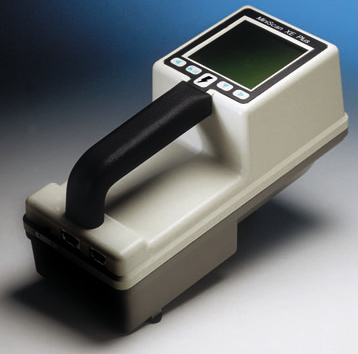
\includegraphics[scale=1]{img/MiniScanXEPlus.png}
			\caption[MiniScan XE Plus]{\textit{MiniScan XE Plus} (Fuente: HunterLab, 2006).}
	\end{figure}
\newpage
\section{Comunicaci\'{o}n con el MiniScan XE Plus}

	Para establecer la comunicaci\'{o}n entre el MiniScan XE Plus y el Spectrasoft, se recurri\'{o} a la documentaci\'{o}n del instrumento, en la cual se describe el MSXE.ocx, un archivo que implementa las funciones comunmente utilizadas por dicho instrumento. Se contact\'{o} al personal de soporte t\'{e}cnico de HunterLab por correo electr\'{o}nico, para solicitarle el c\'{o}digo fuente de dicho archivo y la documentaci\'{o}n relativa a su utilizaci\'{o}n que se pudiera proporcionar para la investigaci\'{o}n.
	
	Si bien el personal no comparti\'{o} el c\'{o}digo fuente del archivo, s\'{i} envi\'{o} la documentaci\'{o}n solicitada y un ejemplo de su uso escrito en Visual Basic for Applications (VBA). Primero se intent\'{o} cargar el archivo y utilizarlo directamente en Qt; sin embargo, ocurr\'{i}a un error de compatibilidad de datos al invocar algunas de sus funciones. La soluci\'{o}n a este problema fue desarrollar una librer\'{i}a escrita en Visual Basic .NET, con la cual se pueden invocar todas las funciones de este archivo sin problema alguno.

	As\'{i} pues, por medio del cable adaptador RS232-USB, y empleando la librer\'{i}a escrita en Visual Basic .NET, se logr\'{o} establecer la comunicaci\'{o}n entre el Spectrasoft y el MiniScan XE Plus.
\newpage
\section{F\'{o}rmulas implementadas}
	A continuaci\'{o}n se muestra el c\'{o}digo fuente de las f\'{o}rmulas de \'{o}ptica y colorimetr\'{i}a que fueron definidas en las bases te\'{o}ricas, e implementadas en el Spectrasoft.
	
	\begin{itemize}
	
	\item \textbf{Funci\'{o}n de \'{i}ndice de eritema:}	
		\begin{lstlisting}
//Calcula el indice de eritema
float eritema(QVector<float> medicion){
    //promRojo: promedio ponderado del color rojo
    float promRojo = (medicion[24]/2.0 + medicion[25]
    + medicion[26] + medicion[27]/2.0)/3.0;

    //promVerde: promedio ponderado del color verde
    float promVerde = (medicion[16]/2.0 + medicion[17]
     + medicion[18]/2.0)/2.0;

    float resultado = 100.0*(log(1.0/promVerde)
     - log(1.0/promRojo));

    return resultado;
}
	\end{lstlisting}
	
\newpage	
	
		\item \textbf{Funci\'{o}n de absorbancia aparente:}
			\begin{lstlisting}
//Calcula los datos de absorbancia aparente
QVector<float> absorbancia(QVector<float> medicion){

	QVector<float> resultado;
	
   	for(int i = 0; i < 31; ++i)
		resultado.push_back(100.0 - medicion[i]);

    return resultado;
}
			\end{lstlisting}
			
		\item \textbf{Funci\'{o}n de coordenadas de cromaticidad CIE xyz:}		
			\begin{lstlisting}
//Calcula las coordenadas de cromaticidad CIE xyz
QVector<float> CIExyz(QVector<float> medicion){
    
    QVector<float> resultado;
    QVector<float> XYZ = CIEXYZ(medicion);
    float x, y, z;

    x = XYZ[0]/(XYZ[0] + XYZ[1] + XYZ[2]);
    y = XYZ[1]/(XYZ[0] + XYZ[1] + XYZ[2]);
    z = XYZ[2]/(XYZ[0] + XYZ[1] + XYZ[2]);

    resultado.push_back(x);
    resultado.push_back(y);
    resultado.push_back(z);

    return resultado;
}
			\end{lstlisting}
			
\newpage
		
		\item \textbf{Funci\'{o}n de valores triest\'{i}mulo CIE XYZ:}
			\begin{lstlisting}
//Calcula los valores triestimulo CIE XYZ
QVector<float> CIEXYZ(QVector<float> medicion){
    
    QVector<float> resultado;
    float auxK, auxX, auxY, auxZ, k, X, Y, Z;

    auxK = auxX = auxY = auxZ = 0.0;

    //realiza las sumatorias indicadas de las formulas
    for(int i = 0; i < 31; ++i){

		auxK+= iluCIED65[i]*yCIE10[i];
        auxX+= medicion[i]*iluCIED65[i]*xCIE10[i];
        auxY+= medicion[i]*iluCIED65[i]*yCIE10[i];
        auxZ+= medicion[i]*iluCIED65[i]*zCIE10[i];
    }

    //calcula la constante k
    k = 100.0/auxK;

    //calcula los valores triestimulo XYZ
    X = k*auxX;
    Y = k*auxY;
    Z = k*auxZ;

    resultado.push_back(X);
    resultado.push_back(Y);
    resultado.push_back(Z);

    return resultado;
}
			\end{lstlisting}

\newpage
		
		\item \textbf{Funci\'{o}n de coordenadas CIELAB:}
			\begin{lstlisting}
//Calcula las coordenadas de del espacio CIELAB
QVector<float> CIELAB(QVector<float> medicion){
    
    QVector<float> resultado;
    QVector<float> XYZ = CIEXYZ(medicion);
    float constante, aux, fXfYfZ[3], L, a, b;

    //calcula la constante utilizada en la formula
    constante = 24.0/116.0;
    constante = pow(constante, 3);

    //calcula las funciones X/Xn, Y/Yn, Z/Zn
    for(int i = 0; i < 3; ++i){

        aux = XYZ[i]/XnYnZn[i];

        if(aux > constante){
            fXfYfZ[i] = pow(aux, 1.0/3.0);
        }else{
            fXfYfZ[i] = (841.0/108.0)*aux + (16.0/116.0);
        }
    }

    //calcula las coordenadas L*a*b*
    L = 116.0*fXfYfZ[1] - 16.0;
    a = 500.0*(fXfYfZ[0] - fXfYfZ[1]);
    b = 200.0*(fXfYfZ[1] - fXfYfZ[2]);

    resultado.push_back(L);
    resultado.push_back(a);
    resultado.push_back(b);

    return resultado;
}
			\end{lstlisting}

\newpage		
		
		\item \textbf{Funci\'{o}n de coeficiente de absorci\'{o}n:}
		
			\begin{lstlisting}
//Calcula el coeficiente de absorcion
QVector<float> absorcion(QVector<float> medicion){

    QVector<float> resultado;
    float rango, aux, Z, k, a0;
    int n, grado;
    bool op = false;//el sistema de ecuaciones a resolver tiene solucion
    
    //son 31 datos, y el grado del polinomio de ajuste es 8
    n = 31; grado = 8;

    double *x = new double[n];
    double *y = new double[n];

    //cargando los datos en x, y
    for(int i = 0; i < n; ++i){
        x[i] = i;
        y[i] = medicion.at(i);
    }

    double **matriz = new double*[grado + 1];

    for (int i = 0; i < grado + 1; ++i)
        matriz[i] = new double[grado + 2];

    //realizando el ajuste polinomial y calculando los coeficientes
    coeficientes(x, y, matriz, grado, n);
    recorrido(matriz, grado + 1, op);

    //a0 esta en la primera fila de la matriz resultante del ajuste
    a0 = matriz[0][grado + 1];
    Z = 0.2796; k = -7.174;
    rango = 400;

    //calculando el coeficiente de absorcion
    for(int i = 0; i < n; ++i){
        aux = Z*exp(k*a0)*6.6*pow(10, 11)*pow(rango, -3.3);
        resultado.push_back(aux);
        rango+=10;
    }

    //liberando la memoria dinamica asiganada
    delete x;
    delete y;

    for(int i = 0; i < grado + 1; ++i)
        delete matriz[i];

    delete matriz;

    return resultado;
}
			\end{lstlisting}

	\end{itemize}

\newpage

\section{Interfaz del software}

	A continuaci\'{o}n se muestran algunas de las ventanas de la interfaz gr\'{a}fica de usuario del Spectrasoft, que comprenden la ventana principal, la ventana de inicio de sesi\'{o}n, la visualizaci\'{o}n de algunos de los resultados de una medici\'{o}n realizada, y los detalles de la historia m\'{e}dica de un paciente.

 \begin{itemize}
 	
 	\item \textbf{Ventana principal:}
 	
 		\begin{figure}[H]
		\centering
		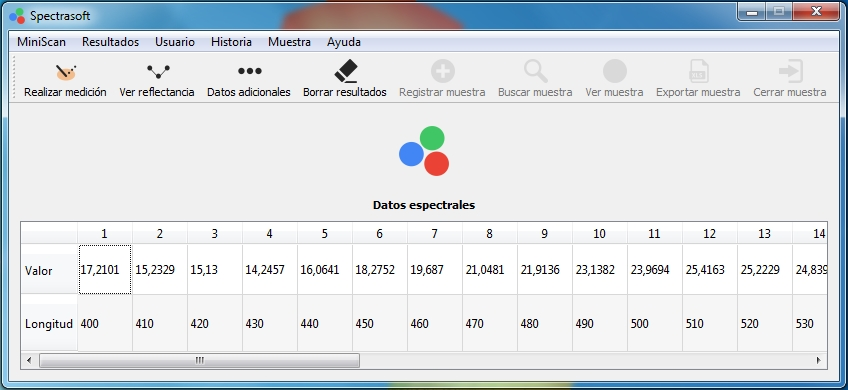
\includegraphics[scale=0.6]{img/vista-principal.jpg}
			\caption[Ventana principal]{\textit{Ventana principal} (Fuente: Autor).}
	\end{figure}
	
	 	\item \textbf{Inicio de sesi\'{o}n:}
 	
 		\begin{figure}[H]
		\centering
		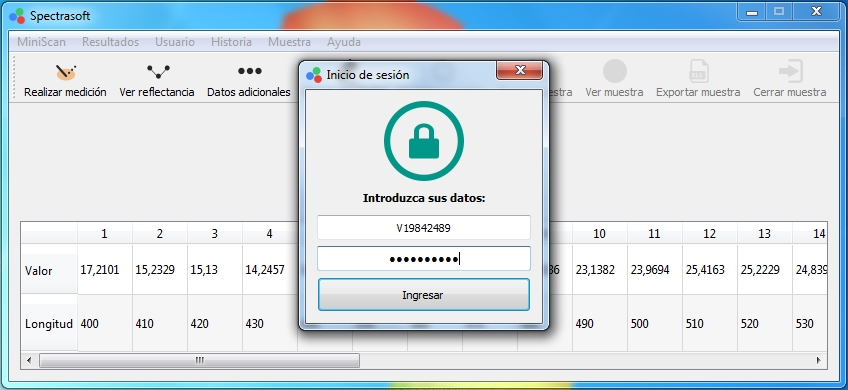
\includegraphics[scale=0.6]{img/vista-inicio-sesion.jpg}
			\caption[Inicio de sesi\'{o}n]{\textit{Inicio de sesi\'{o}n} (Fuente: Autor).}
	\end{figure}

\newpage
	 	\item \textbf{Curva de reflectancia:}
 	
 		\begin{figure}[H]
		\centering
		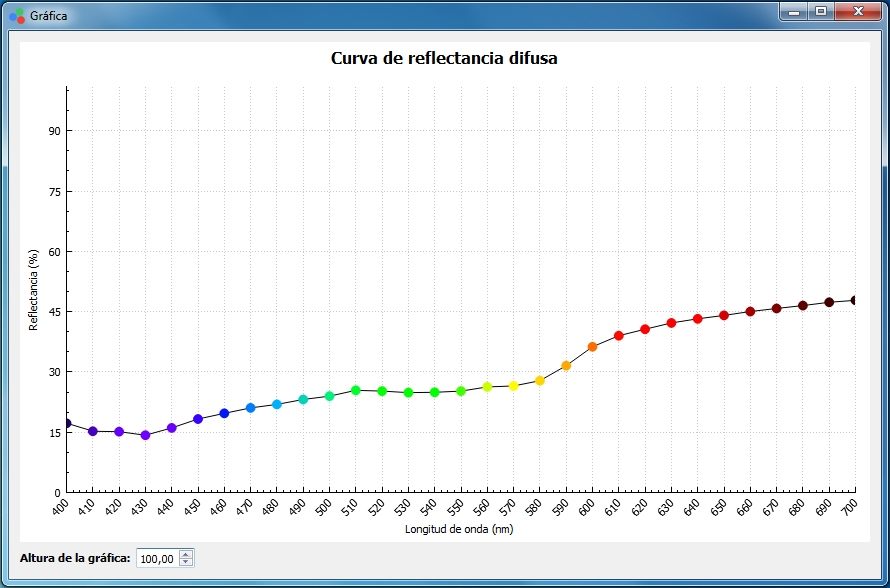
\includegraphics[scale=0.55]{img/vista-reflectancia.jpg}
			\caption[Curva de reflectancia]{\textit{Curva de reflectancia} (Fuente: Autor).}
	\end{figure}
	
		 	\item \textbf{Historia m\'{e}dica de un paciente:}
 	
 		\begin{figure}[H]
		\centering
		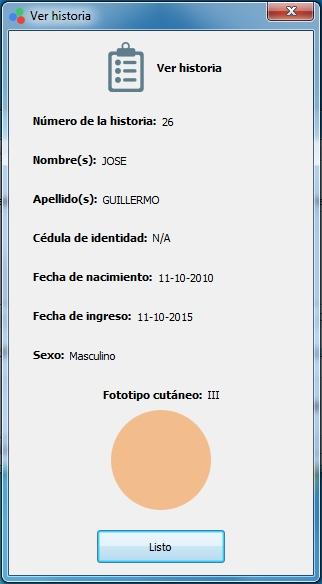
\includegraphics[scale=0.65]{img/vista-historia.jpg}
			\caption[Historia m\'{e}dica de un paciente]{\textit{Historia m\'{e}dica de un paciente} (Fuente: Autor).}
	\end{figure}

\end{itemize}

\newpage
\section{Manuales}
	Se gener\'{o} un manual de instalaci\'{o}n que detalla todos los pasos que se deben seguir para instalar y configurar todo lo necesario para instalar y ejecutar el Spectrasoft, as\'{i} como la instalaci\'{o}n del mismo. Adem\'{a}s se realiz\'{o} un manual de usuario, en donde se explica con detalle la permisolog\'{i}a de los usuarios del Spectrasoft y las funciones que dicho software ofrece. Estos manuales est\'{a}n disponibles en los anexos A y B.

\section{Pruebas realizadas}
	
	El desarrollo de un software incluye verificar y validar que \'{e}ste se encuentre libre de errores y que se haya logrado el objetivo de su dise\~{n}o. En este sentido, se realizaron pruebas de funcionalidad empleando el modelo de guiones de prueba y de pruebas de aceptaci\'{o}n propuestos por \citeA{INSITE}, cuyos resultados permitieron determinar que el software Spectrasoft cumple con todos los requerimientos y objetivos definidos.
	
	Las pruebas de usabilidad se realizaron utilizando las heur\'{i}sticas de \citeA{Nielsen}, tomando \'{u}nicamente los \'{i}tems de evaluaci\'{o}n que se pudieran aplicar en el software y adapt\'{a}ndolos para ese fin; dichas pruebas de usabilidad mostraron que el software Spectrasoft cumple con el atributo de usabilidad, necesario para ser considerado un software de calidad. Tales pruebas y las constancias de aceptaci\'{o}n firmadas por los clientes est\'{a}n disponibles en los anexos comprendidos desde el C, hasta el F.
	
	\subsection{C\'{a}lculo de los valores triest\'{i}mulo CIE XYZ}
	Para verificar que la implementaci\'{o}n de la f\'{o}rmula para calcular los valores triest\'{i}mulo CIE XYZ	es correcta, se realiz\'{o} una medici\'{o}n a la placa de diagn\'{o}stico de HunterLab con el MiniScan XE Plus, utilizando el Spectrasoft para calcular los valores triest\'{i}mulo de la misma. Esta placa proporciona valores triest\'{i}mulo de control, los cuales fueron le\'{i}dos de f\'{a}brica utilizando el iluminante est\'{a}ndar D65 y el observador est\'{a}ndar de 10\degree. Al comparar los valores triest\'{i}mulo calculados por el Spectrasoft con los valores triest\'{i}mulo de control de la placa, se puede observar que los valores se asemejan. La tabla 4.6 muestra los valores comparados.
	
	\begin{table}[h]
		\small
		\caption[Verificaci\'{o}n de los valores triest\'{i}mulo CIE XYZ]{\textit{Verificaci\'{o}n de los valores triest\'{i}mulo CIE XYZ} (Fuente: Autor).}
		\centering
		\setlength{\extrarowheight}{\altocelda}
		\begin{tabulary}{\anchotabla}{|c|c|}
			\hline
			\thead{\textbf{\small{Valores de control}}} & \thead{\textbf{\small{Valores del Spectrasoft}}}\\ \hline
			$X = 18.6$ & $X = 17.72$\\ \hline
			$Y = 24.5$ & $Y = 23.51$\\ \hline
			$Z = 20.7$ & $Z = 20.01$\\ \hline
		\end{tabulary}
	\end{table}
	
	\subsection{Realizaci\'{o}n de las mediciones}
		Para corroborar que las mediciones realizadas utilizando con el Spectrasoft generan los mismos resultados que las mediciones realizadas con el HunterLab Universal Software, se realiz\'{o} la medici\'{o}n de una muestra en una misma zona dos veces, la primera utilizando el Spectrasoft, y la segunda utilizando el HunterLab Universal Software. En las figuras 4.14 y 4.15 se puede observar que las curvas de reflectancia difusa resultantes de las mediciones tienen la misma forma, por lo que las mediciones realizadas con el Spectrasoft son correctas.
	\newpage
		
 	\begin{figure}[H]
		\centering
		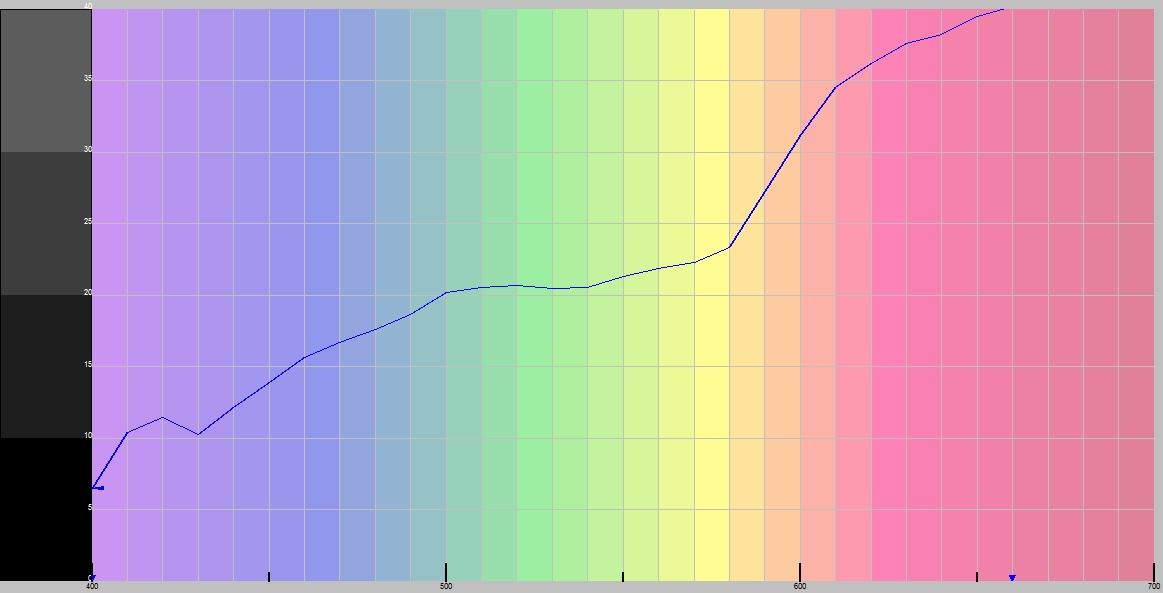
\includegraphics[scale=0.45]{img/medicion-hunterlab.jpg}
			\caption[Medici\'{o}n del HunterLab Universal Software]{\textit{Medici\'{o}n del HunterLab Universal Software} (Fuente: CIMBUC, 2015).}
	\end{figure}	
	
 	\begin{figure}[H]
		\centering
		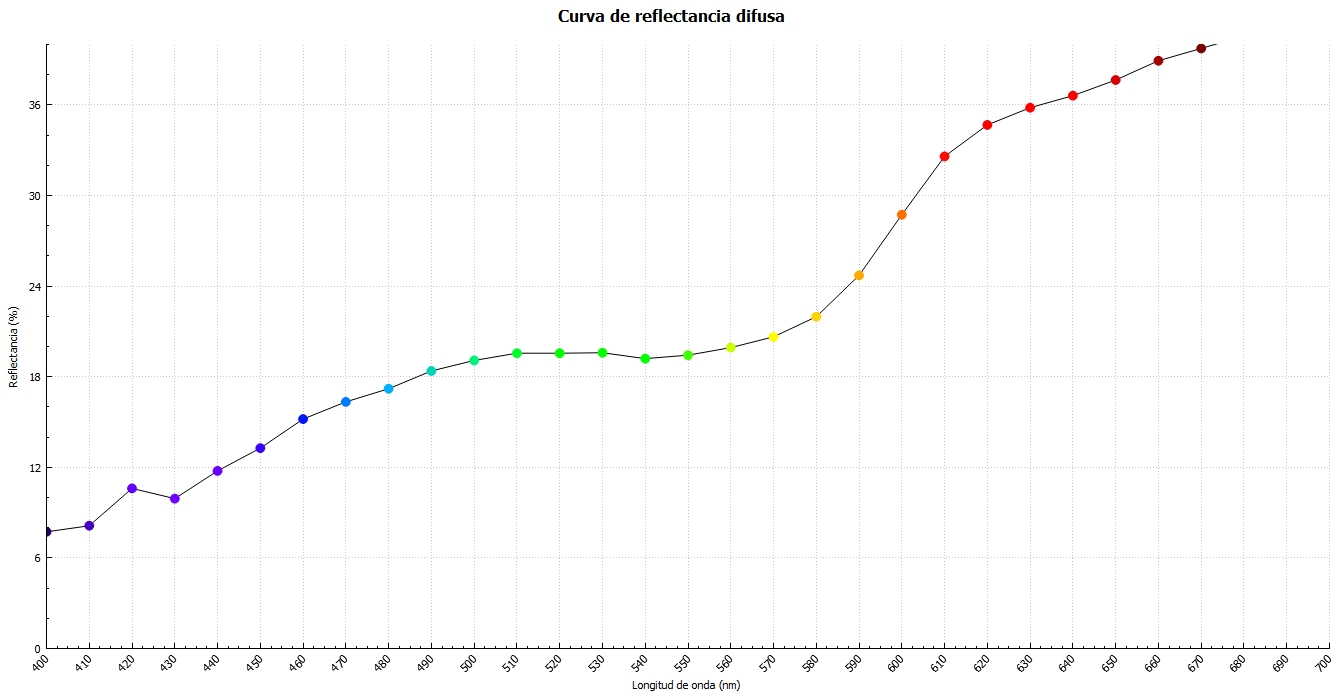
\includegraphics[scale=0.4]{img/medicion-spectrasoft.jpg}
			\caption[Medici\'{o}n del Spectrasoft]{\textit{Medici\'{o}n del Spectrasoft} (Fuente: Autor).}
	\end{figure}
	
\subsection{C\'{a}lculo de las f\'{o}rmulas restantes}

	\begin{itemize}
		
		\item \textbf{Absorbancia aparente:} No hay forma de determinar con exactitud la luz que es absorbida por un medio, por esta raz\'{o}n se asume que la luz que no es reflejada de vuelta al MiniScan XE Plus, debe ser la luz que es aparentemente absorbida. Por esta raz\'{o}n esta f\'{o}rmula no es verificada.
	
		\item \textbf{Coordenadas tricrom\'{a}ticas CIE xyz:} La f\'{o}rmula utilizada para calcular estas coordenadas es una normalizaci\'{o}n de los valores triest\'{i}mulo CIE XYZ, y estos \'{u}ltimos ya fueron verificados, por lo que no hace falta realizar la verificaci\'{o}n de estas coordenadas.
		
		\item \textbf{Coordenadas del espacio CIELAB:} La f\'{o}rmula utilizada para calcular estas coordenadas no es m\'{a}s que la transformaci\'{o}n de los valores triest\'{i}mulo CIE XYZ, raz\'{o}n por la cual no hace falta realizar su verificaci\'{o}n.
		
		\item \textbf{Coeficiente de absorci\'{o}n:} La f\'{o}rmula utilizada para determinar este coeficiente es la definida por \citeA{Narea}, en cuyo art\'{i}culo deja documentadas las pruebas y los an\'{a}lisis relacionados con la misma, por este motivo esta f\'{o}rmula no es verificada.
		
		\item \textbf{\'{I}ndice de eritema:} La f\'{o}rmula utilizada para determinar este \'{i}ndice es la definida por \citeA{Wagner}, en cuyo art\'{i}culo deja documentadas las pruebas y los an\'{a}lisis relacionados con la misma, por esta raz\'{o}n no es verificada.
	\end{itemize}
	
\section{Colores utilizados en el software}

	Es importante destacar que los colores utilizados en las gr\'{a}ficas generadas por el Spectrasoft son referencias visuales, por lo tanto no son una reproducci\'{o}n real de los colores que representan. De la misma manera, los colores utilizados para representar los fototipos de piel en el Spectrasoft son solamente referencias visuales de la escala propuesta por \citeA{Fitzpatrick}.
	\chapter{Conclusiones y recomendaciones}

\section{Conclusiones}

	La elaboraci\'{o}n de la presente investigaci\'{o}n ha cumplido los objetivos planteados. Para lograr esto fue necesario un an\'{a}lisis detallado de la bibliograf\'{i}a, la revisi\'{o}n de algunas investigaciones previas, y el estudio riguroso del material proporcionado por el personal de soporte t\'{e}cnico de la empresa HunterLab.
	
	El aporte general de este trabajo de investigaci\'{o}n se centra en proveer un software libre para operar el MiniScan XE Plus, el cual dispone de las funciones necesarias para que los dermat\'{o}logos puedan establecer diagn\'{o}sticos de patolog\'{i}as dermatol\'{o}gicas en pacientes.
	
	Desde el comienzo del proceso de desarrollo del software se opt\'{o} por trabajar con un servicio gratuito de control de versiones, lo cual permiti\'{o} tener almacenado el c\'{o}digo fuente del software de manera centralizada. Esto ayud\'{o} a tener una mejor organizaci\'{o}n durante el desarrollo.
	
	Debido a las limitaciones encontradas durante la investigaci\'{o}n, se concluye que es necesaria la utilizaci\'{o}n de algunos archivos de HunterLab para lograr la comunicaci\'{o}n entre el software resultante y el MiniSan XE Plus. Adicionalmente, debido a esta limitaci\'{o}n el software resultante no puede captar ni interpretar las se\~{n}ales de los botones del MiniScan XE Plus, ya que estos archivos no ofrecen esta caracter\'{i}stica para ser utilizada fuera del HunterLab Universal Software.
	
	La instalaci\'{o}n de este software no es tan simple como podr\'{i}a llegar a ser, como consecuencia de la necesidad de utilizar algunos archivos del HunterLab. El software resultante no puede habilitarse para ser multiplataforma debido a esta raz\'{o}n.

	Durante las pruebas de funcionalidad y usabilidad realizadas al software se hizo notorio el nivel de aceptaci\'{o}n y la satisfacci\'{o}n de los clientes a los que iba dirigido. Adicionalmente, se realiz\'{o} un manual de usuario para la correcta utilizaci\'{o}n del software, que explica detalladamente con tablas y con im\'{a}genes la permisolog\'{i}a de sus usuarios y las funciones que ofrece, por lo que su curva de aprendizaje es baja.

	En definitiva, se concluye que el software resultante cumple con todos los objetivos establecidos en esta investigaci\'{o}n, ajustandose a las necesidades de los dermat\'{o}logos, garantizando un mejor aprovechamiento del MiniScan XE Plus, creando una base sobre la cual se pueden realizar trabajos futuros que modifiquen, mejoren y extiendan dicho software.

\newpage

\section{Recomendaciones}

	De acuerdo a las conclusiones alcanzadas con el trabajo, se han generado una serie de recomendaciones, las cuales se presentan a continuaci\'{o}n.

\begin{itemize}

	\item Permitir la visualizaci\'{o}n, consulta y exportaci\'{o}n de varias muestras al mismo tiempo.
	
	\item Desarrollar un arhivo controlador para el MiniScan XE Plus que no dependa del kit MSXE.ocx del HunterLab, para as\'{i} simplificar el proceso de instalaci\'{o}n del Spectrasoft, lograr que el mismo sea capaz de captar e interpretar las se\~{n}ales de los botones del MiniScan XE Plus, y posibilitar que \'{e}ste sea multiplataforma.
	
	\item Incluir la f\'{o}rmula desarrollada por los investigadores del CIMBUC para el c\'{a}lculo del coeficiente de esparcimiento de la epidermis, la cual no estuvo lista durante el tiempo en el que se llev\'{o} a cabo este trabajo de investigaci\'{o}n.
	
	\item Crear una nueva base de datos que habilite la gesti\'{o}n de muestras experimentales para los investigadores del CIMBUC.
	
	\item Adaptar el Spectrasoft a una arquitectura de modelo cliente-servidor para permitir la conexi\'{o}n con bases de datos remotas en sistemas distribuidos.
	
	\item Disponer de un ambiente \textit{QA} para realizar pruebas de rendimiento y de base de datos al Spectrasoft, previas a su puesta en producci\'{o}n.
	
	\item Incluir la carga de muestras por archivo al Spectrasoft.
\end{itemize}
	\nocite{*}
	\renewcommand\bibname{Referencias}
	\bibliography{bibliografia}

	\titleformat{\chapter}[hang]
	{\normalfont\bfseries}{\chaptertitlename\ \thechapter:}{1em}{}
	\makeatletter
	\def\ttl@mkchap@i#1#2#3#4#5#6#7{%
    \ttl@assign\@tempskipa#3\relax\beforetitleunit
    \vspace{\@tempskipa}%<<<<<< REMOVE THE * AFTER \vspace
    \global\@afterindenttrue
    \ifcase#5 \global\@afterindentfalse\fi
    \ttl@assign\@tempskipb#4\relax\aftertitleunit
    \ttl@topmode{\@tempskipb}{%
        \ttl@select{#6}{#1}{#2}{#7}}%
    \ttl@finmarks  % Outside the box!
    \@ifundefined{ttlp@#6}{}{\ttlp@write{#6}}}
    \makeatother
	\appendix
\clearpage
\addappheadtotoc
\appendixpage

\chapter{Manual de instalaci\'{o}n}
\thispagestyle{fancy}
\section*{Requerimientos del sistema}

\subsection*{Requerimientos de hardware}

	\begin{itemize}
		\item Procesador de 1 gigahertz (GHz) o superior.
		
		\item 1 gigabyte (GB) de memoria RAM o m\'{a}s.
		
		\item Resoluci\'{o}n de pantalla de 1024x768 o superior.
	\end{itemize}
	
\subsection*{Requerimientos de arquitectura}

	\begin{itemize}
		\item Arquitectura de 32 bits o de 64 bits.
	\end{itemize}

\subsection*{Requerimientos del sistema operativo}

	\begin{itemize}
		\item Sistema operativo Microsoft Windows 7 Service Pack 1 o superior.
	\end{itemize}
	
\subsection*{Requerimientos de software}

	\begin{itemize}
		\item Microsoft .NET framework 4 o superior.
		
		\item Microsoft Internet Explorer 10 o superior.
	\end{itemize}

\newpage

\section*{Acciones previas}

	\subsection*{Controlador para el adaptador serial-USB}
	
	Conecte el MiniScan XE Plus utilizando el cable adaptador serial-USB, luego instale el controlador para el adaptador dejando todas las opciones de instalaci\'{o}n por defecto.

	\subsection*{Paquete MSXP-CFLX Utility}
	
	Instale el paquete MSXP-CFLX Utility, ejecut\'{a}ndolo como administrador y dejando todas las opciones de instalaci\'{o}n por defecto.
	
	\subsection*{Carpeta MSXEBridge}
	
	Copie la carpeta <<MSXEBridge>> en el disco local C, en la ruta <<C:\textbackslash>>.
	
\section*{Versiones de los paquetes a instalar}

\begin{itemize}
	\item Visual Studio 2013 community/professional/ultimate.
	
	\item PostgreSQL 9.4.4-3.
\end{itemize}

\newpage

\section*{Instalaci\'{o}n de Visual Studio}
	
Ejecute la instalaci\'{o}n de Visual Studio como administrador. Seleccione la opci\'{o}n <<Acepto los t\'{e}rminos de licencia y la declaraci\'{o}n de privacidad.>> y haga click en el bot\'{o}n <<Siguiente>> (v\'{e}ase la figura \ref{fig:vs-instalacion1}).

\begin{figure}[H]
  \centering
  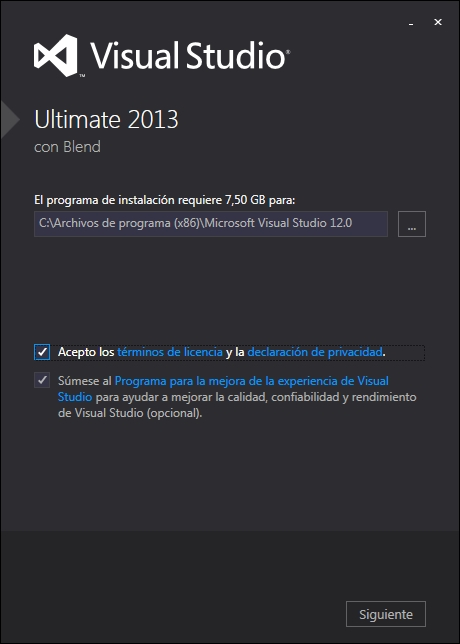
\includegraphics[width=.8\linewidth]{./img/vs-instalacion1.jpg}
\caption[]{Inicio de instalaci\'{o}n de Visual Studio\label{fig:vs-instalacion1}}
\end{figure}
\newpage
Deje todas las opciones por defecto de <<Caracter\'{i}sticas opcionales para instalar:>> y haga click en el bot\'{o}n <<INSTALAR>> (v\'{e}ase la figura \ref{fig:vs-instalacion2}).	

\begin{figure}[H]
  \centering
  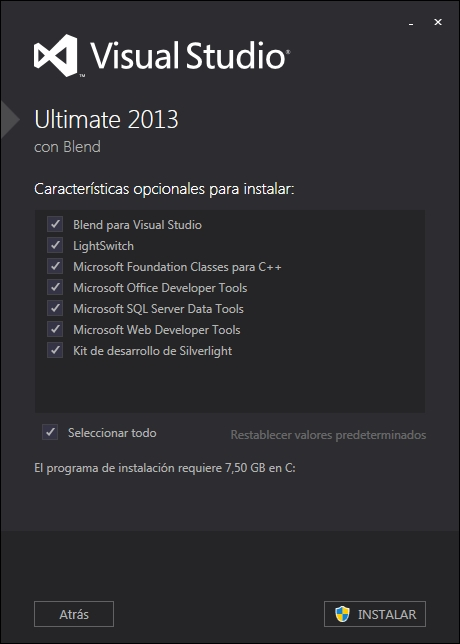
\includegraphics[width=.8\linewidth]{./img/vs-instalacion2.jpg}
\caption[]{Caracter\'{i}sticas opcionales de Visual Studio\label{fig:vs-instalacion2}}
\end{figure}
\newpage
Espere a que el proceso de instalaci\'{o}n finalice (v\'{e}ase la figura \ref{fig:vs-instalacion3}).	

\begin{figure}[H]
  \centering
  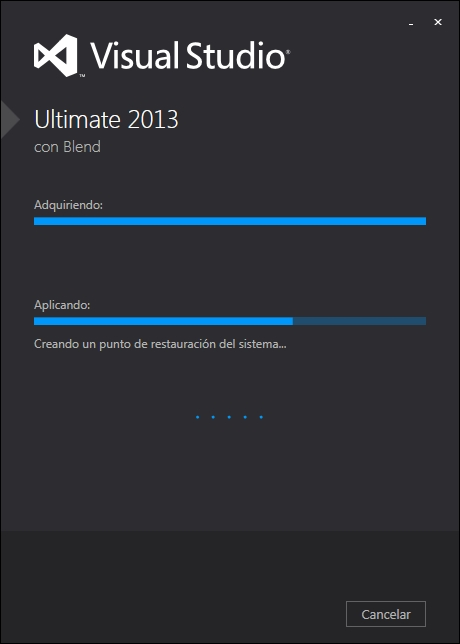
\includegraphics[width=.8\linewidth]{./img/vs-instalacion3.jpg}
\caption[]{Progreso de la instalaci\'{o}n de Visual Studio\label{fig:vs-instalacion3}}
\end{figure}
\newpage
Despu\'{e}s de finalizar la instalaci\'{o}n, no inicie Visual Studio, haga click en el bot\'{o}n con forma de equis (x) en la esquina superior para cerrar la ventana (v\'{e}ase la figura \ref{fig:vs-instalacion4}).	

\begin{figure}[H]
  \centering
  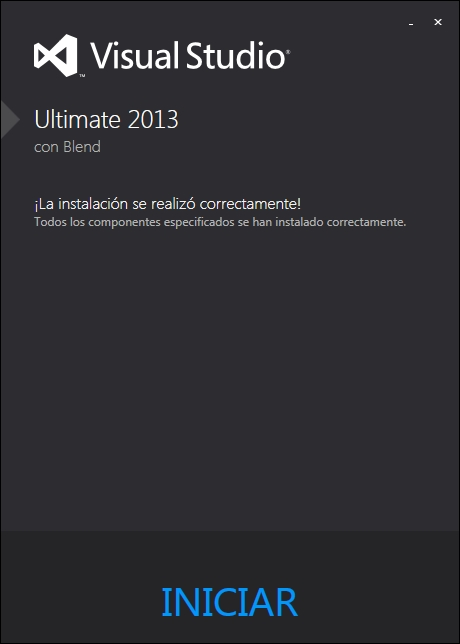
\includegraphics[width=.8\linewidth]{./img/vs-instalacion4.jpg}
\caption[]{Cerrar ventana de instalaci\'{o}n de Visual Studio\label{fig:vs-instalacion4}}
\end{figure}

\newpage

\section*{Instalaci\'{o}n de PostgreSQL}
	
Ejecute la instalaci\'{o}n de PostgreSQL como administrador. Haga click en el bot\'{o}n <<Siguiente>> (v\'{e}ase la figura \ref{fig:postgres1}).

\begin{figure}[H]
  \centering
  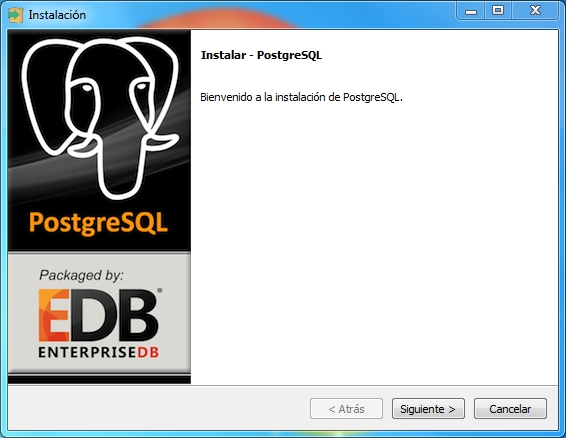
\includegraphics[width=.6\linewidth]{./img/postgres1.jpg}
\caption[]{Inicio de instalaci\'{o}n de PostgreSQL\label{fig:postgres1}}
\end{figure}

Deje la ubicaci\'{o}n del directorio de instalaci\'{o}n por defecto y haga click en el bot\'{o}n <<Siguiente>> (v\'{e}ase la figura \ref{fig:postgres2}).

\begin{figure}[H]
  \centering
  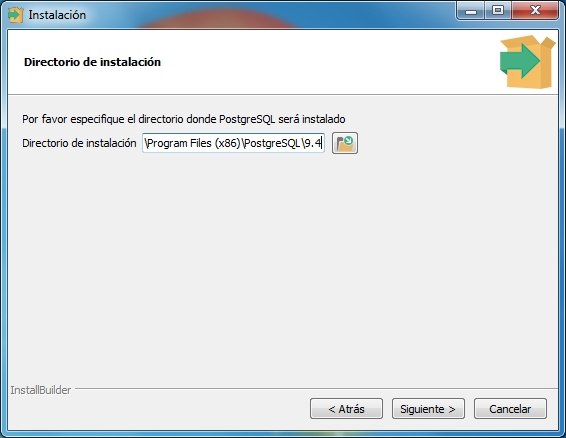
\includegraphics[width=.6\linewidth]{./img/postgres2.jpg}
\caption[]{Directorio de instalaci\'{o}n de PostgreSQL\label{fig:postgres2}}
\end{figure}

\newpage

Deje la ubicaci\'{o}n del directorio de datos por defecto y haga click en el bot\'{o}n <<Siguiente>> (v\'{e}ase la figura \ref{fig:postgres3}).

\begin{figure}[H]
  \centering
  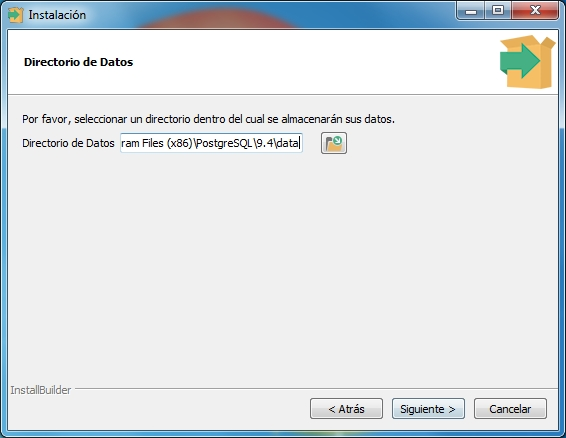
\includegraphics[width=.6\linewidth]{./img/postgres3.jpg}
\caption[]{Inicio de datos de PostgreSQL\label{fig:postgres3}}
\end{figure}

Introduzca una contrase\~{n}a de su preferencia, gu\'{a}rdela en un lugar seguro y haga click en el bot\'{o}n <<Siguiente>> (v\'{e}ase la figura \ref{fig:postgres4}).

\begin{figure}[H]
  \centering
  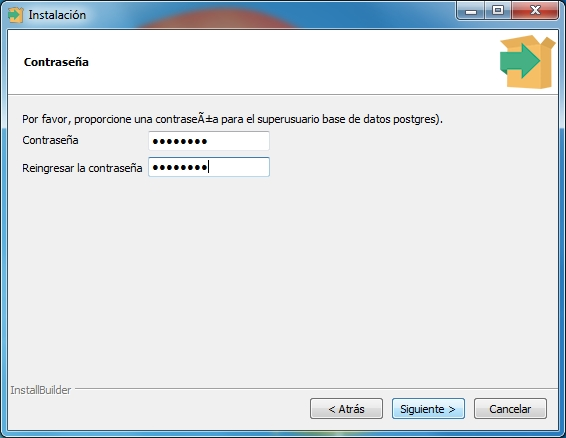
\includegraphics[width=.6\linewidth]{./img/postgres4.jpg}
\caption[]{Contrase\~{n}a para el superusuario de PostgreSQL\label{fig:postgres4}}
\end{figure}

\newpage

Deje el n\'{u}mero del puerto por defecto y haga click en el bot\'{o}n <<Siguiente>> (v\'{e}ase la figura \ref{fig:postgres5}).

\begin{figure}[H]
  \centering
  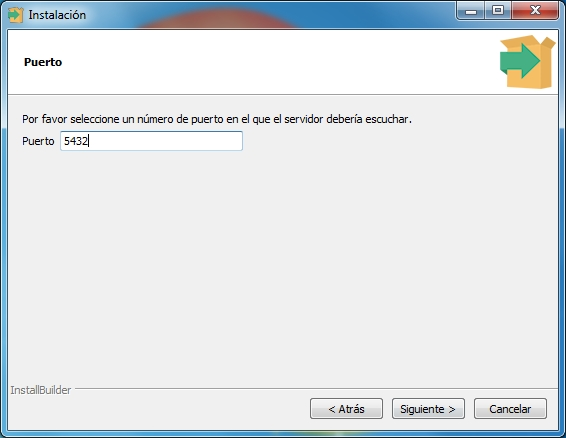
\includegraphics[width=.6\linewidth]{./img/postgres5.jpg}
\caption[]{N\'{u}mero de puerto para PostgreSQL\label{fig:postgres5}}
\end{figure}

Deje la configuraci\'{o}n regional por defecto y haga click en el bot\'{o}n <<Siguiente>> (v\'{e}ase la figura \ref{fig:postgres6}).

\begin{figure}[H]
  \centering
  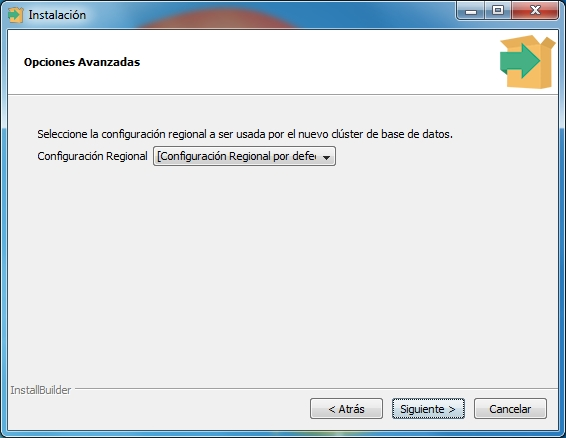
\includegraphics[width=.6\linewidth]{./img/postgres6.jpg}
\caption[]{Configuraci\'{o}n regional para PostgreSQL\label{fig:postgres6}}
\end{figure}

\newpage

Haga click en el bot\'{o}n <<Siguiente>> para empezar el proceso de instalaci\'{o}n y espere a que finalice (v\'{e}ase las figuras \ref{fig:postgres7} y \ref{fig:postgres8}).

\begin{figure}[H]
  \centering
  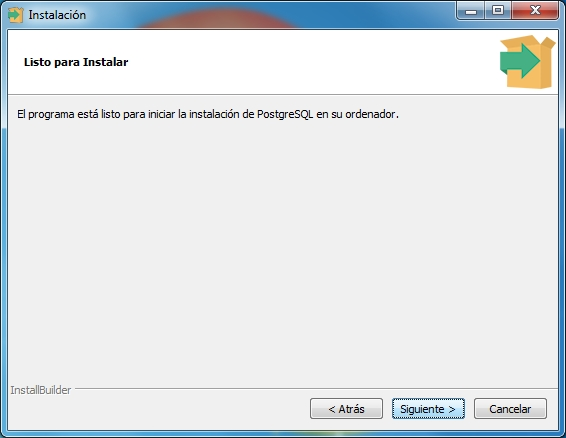
\includegraphics[width=.7\linewidth]{./img/postgres7.jpg}
\caption[]{Inicio de la instalaci\'{o}n de PostgreSQL\label{fig:postgres7}}
\end{figure}

\begin{figure}[H]
  \centering
  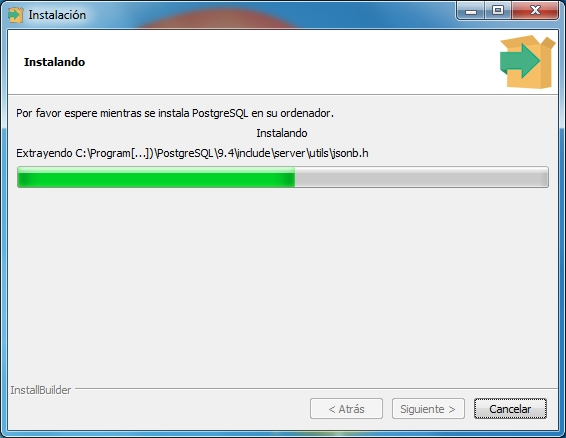
\includegraphics[width=.7\linewidth]{./img/postgres8.jpg}
\caption[]{Proceso de instalaci\'{o}n de PostgreSQL\label{fig:postgres8}}
\end{figure}

\newpage

Despu\'{e}s de finalizar la instalaci\'{o}n, aseg\'{u}rese de que la opci\'{o}n <<Lanzar Stack Builder al finalizar>> no este seleccionada, y por \'{u}ltimo haga click en el bot\'{o}n <<Terminar>> (v\'{e}ase la figura \ref{fig:vs-instalacion9}).	

\begin{figure}[H]
  \centering
  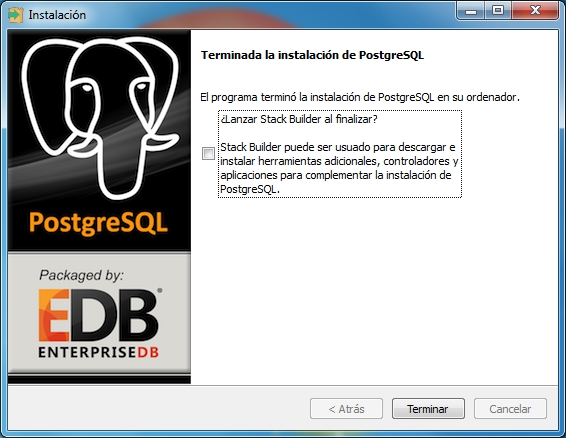
\includegraphics[width=.8\linewidth]{./img/postgres9.jpg}
\caption[]{Finalizaci\'{o}n de la instalaci\'{o}n de PostgreSQL\label{fig:vs-instalacion9}}
\end{figure}

\newpage

\section*{Configuraci\'{o}n de Visual Studio}
	
	Ejecute el software Visual Studio como administrador. En caso de que al iniciar se le pregunte si desea iniciar sesi\'{o}n, elija la opci\'{o}n <<De momento no, quiz\'{a}s m\'{a}s tarde>> (v\'{e}ase la figura \ref{fig:vs-inicio}).	

\begin{figure}[H]
  \centering
  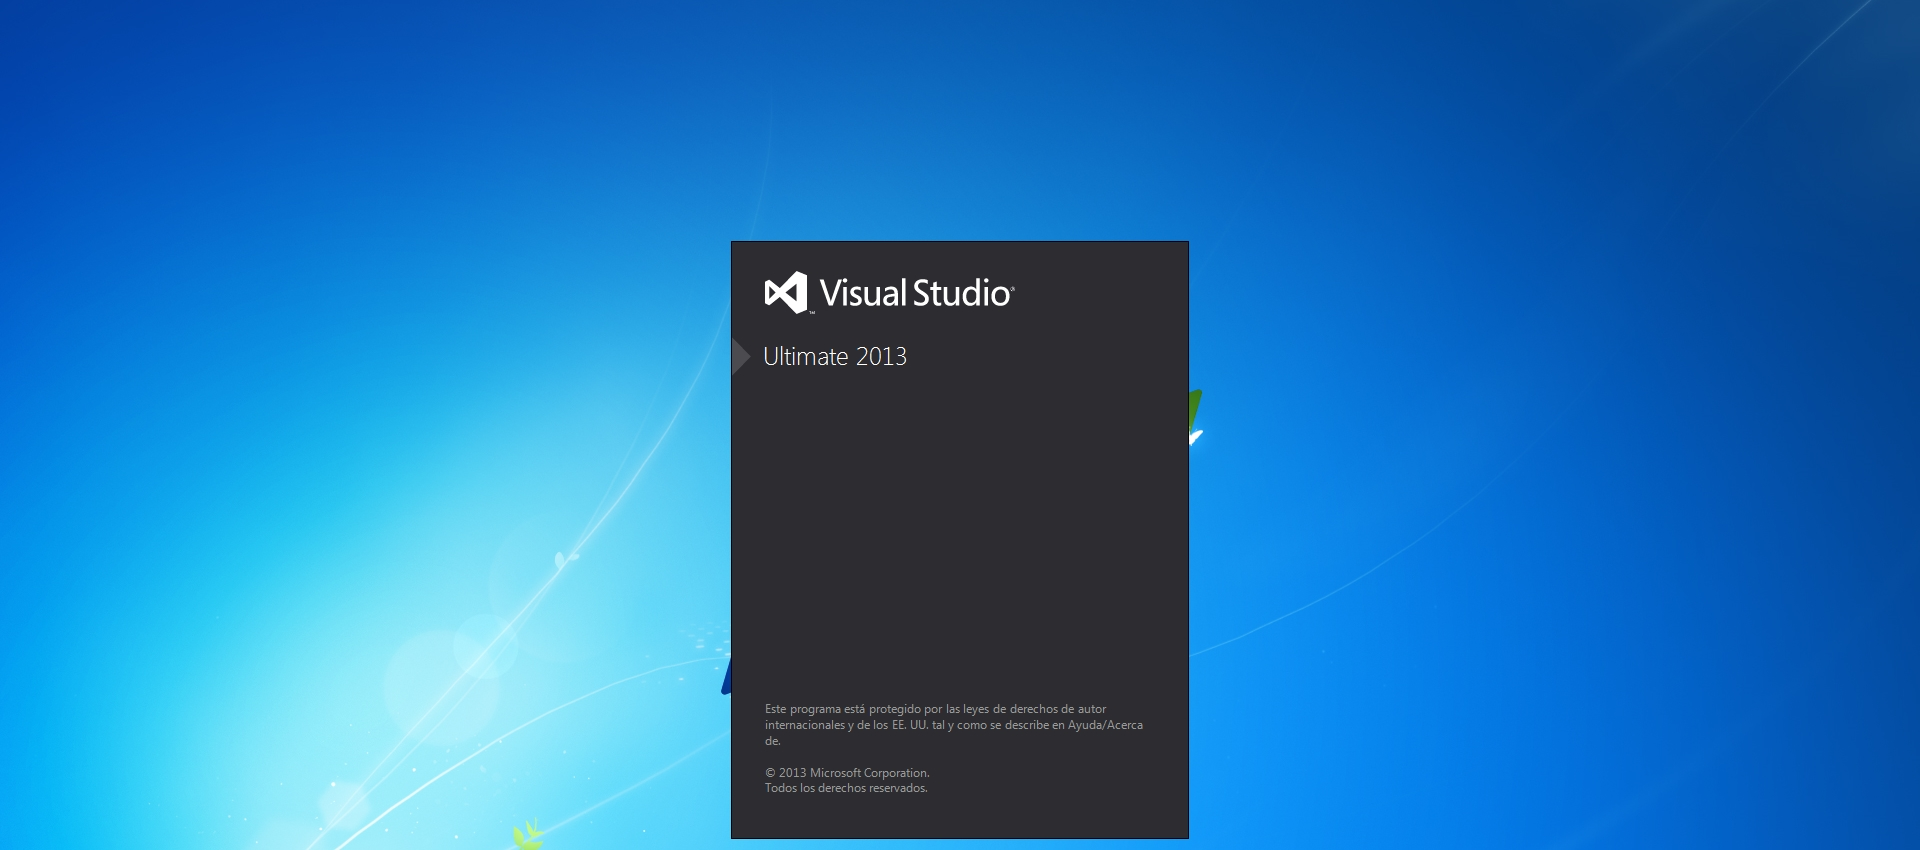
\includegraphics[width=.8\linewidth]{./img/vs-inicio.jpg}
\caption[]{Vista de inicio de Visual Studio\label{fig:vs-inicio}}
\end{figure}

En el men\'{u} <<ARCHIVO>> entre al submen\'{u} <<Abrir>> y haga click en la opci\'{o}n <<Proyecto o soluci\'{o}n...>> (v\'{e}ase la figura \ref{fig:vs-abrir}).	

\begin{figure}[H]
  \centering
  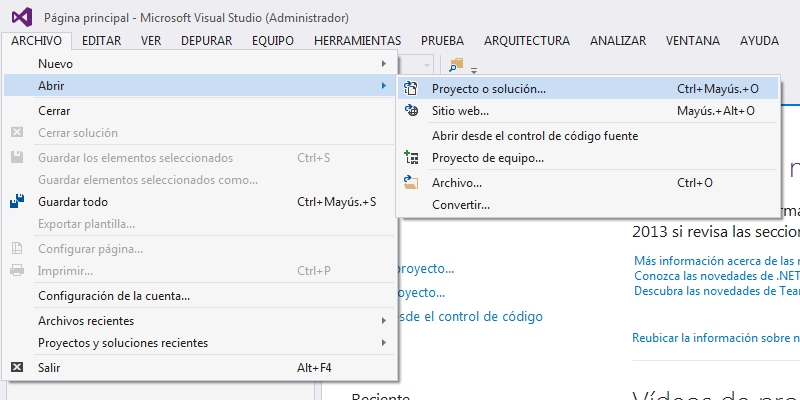
\includegraphics[width=.8\linewidth]{./img/vs-proyecto-abrir.jpg}
\caption[]{Abrir proyecto\label{fig:vs-abrir}}
\end{figure}

\newpage

En la carpeta <<MSXEBridge>> ubicada en el disco <<C:\textbackslash>>, seleccione el archivo <<MSXEBridge>> y haga click en el bot\'{o}n <<Abrir>> (v\'{e}ase la figura \ref{fig:vs-abrir-buscar}).

\begin{figure}[H]
  \centering
  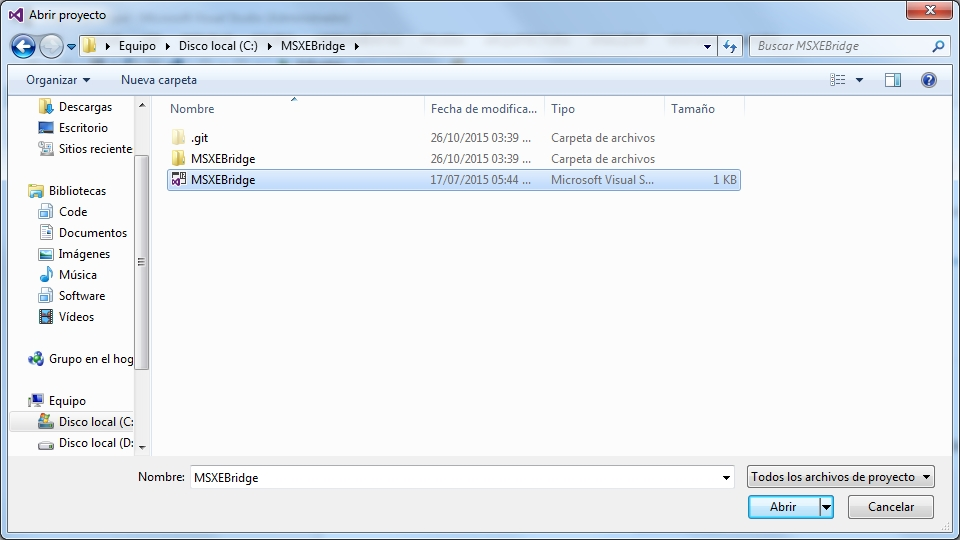
\includegraphics[width=.8\linewidth]{./img/vs-abrir-buscar.jpg}
\caption[]{Buscar el archivo MSXEBridge\label{fig:vs-abrir-buscar}}
\end{figure}

En la parte derecha de Visual Studio, haga click con el bot\'{o}n derecho en <<MSXEBridge>> y seleccione la opci\'{o}n <<Propiedades>> (v\'{e}ase la figura \ref{fig:vs-propiedades}).

\begin{figure}[H]
  \centering
  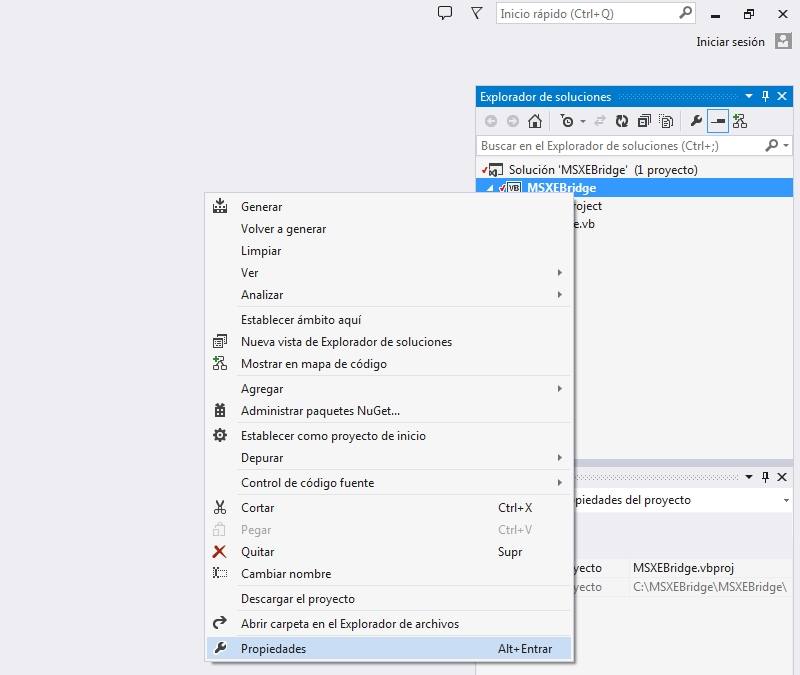
\includegraphics[width=.7\linewidth]{./img/vs-propiedades.jpg}
\caption[]{Propiedades de MSXEBridge\label{fig:vs-propiedades}}
\end{figure}

\newpage

Haga click al bot\'{o}n <<Informaci\'{o}n de ensamblado...>>, aseg\'{u}rese de que la opci\'{o}n <<Crear ensamblado visible a trav\'{e}s de COM>> est\'{e} seleccionada, y haga click en el bot\'{o}n <<Aceptar>> (v\'{e}ase la figura \ref{fig:vs-ensamblado}).

\begin{figure}[H]
  \centering
  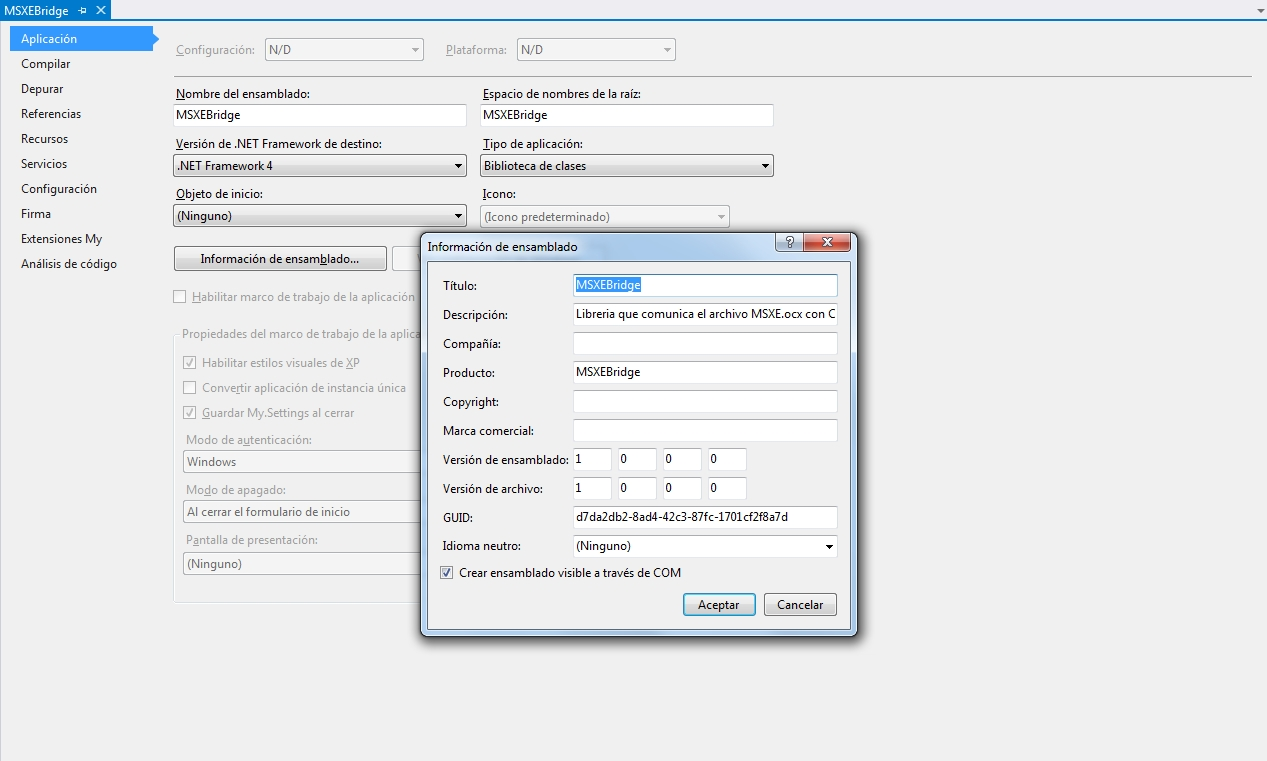
\includegraphics[width=.75\linewidth]{./img/vs-ensamblado.jpg}
\caption[]{Ensamblado de MSXEBridge\label{fig:vs-ensamblado}}
\end{figure}

Haga click en la pesta\~{n}a <<Compilar>> y aseg\'{u}rese de que la opci\'{o}n <<Registrar para interoperabilidad COM>> est\'{e} seleccionada (v\'{e}ase la figura \ref{fig:vs-compilar}).

\begin{figure}[H]
  \centering
  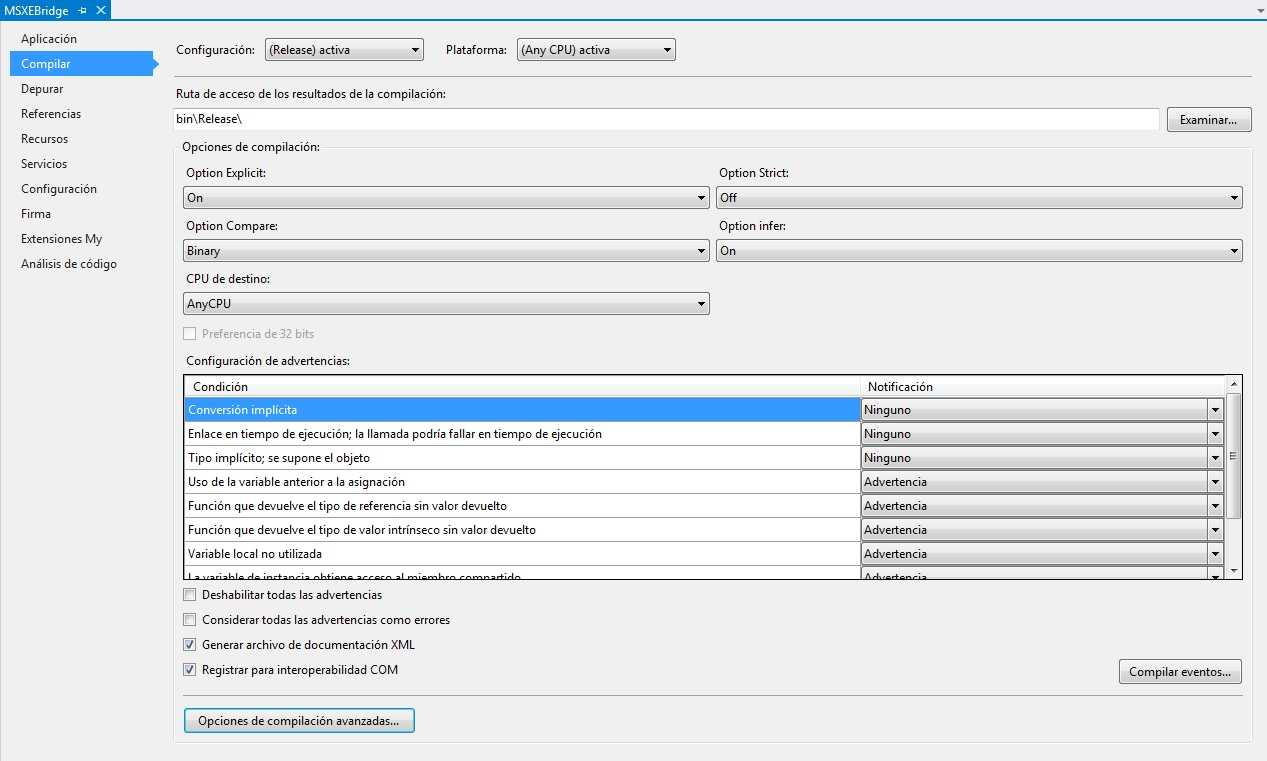
\includegraphics[width=.75\linewidth]{./img/vs-compilar.jpg}
\caption[]{Interoperabilidad de MSXEBridge\label{fig:vs-compilar}}
\end{figure}

\newpage

En el men\'{u} <<COMPILAR>>, haga click en la opci\'{o}n <<Compilar soluci\'{o}n>> est\'{e} seleccionada (v\'{e}ase la figura \ref{fig:vs-compilar-solucion}).

\begin{figure}[H]
  \centering
  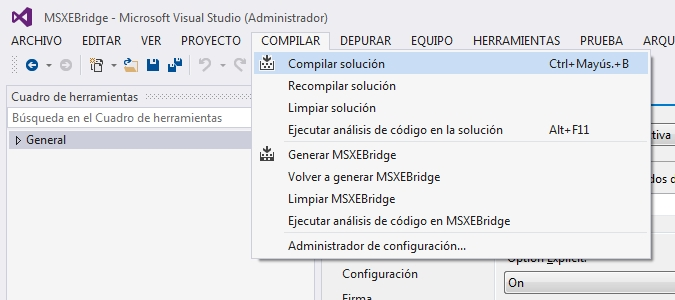
\includegraphics[width=1\linewidth]{./img/vs-compilar-solucion.jpg}
\caption[]{Compilar MSXEBridge\label{fig:vs-compilar-solucion}}
\end{figure}

En la parte inferior de Visual Studio podr\'{a} ver que la compilaci\'{o}n finaliz\'{o} correctamente (v\'{e}ase la figura \ref{fig:vs-resultados}). Por \'{u}ltimo, cierre el software Visual Studio.

\begin{figure}[H]
  \centering
  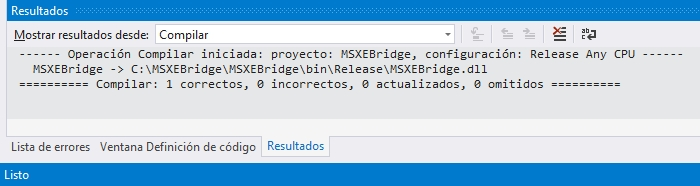
\includegraphics[width=1\linewidth]{./img/vs-resultados.jpg}
\caption[]{Resultados de la compilaci\'{o}n\label{fig:vs-resultados}}
\end{figure}

Es importante destacar que los pasos seguidos previamente s\'{o}lo se deben realizar una vez, y no es necesario que ejecute Visual Studio posteriormente para ejecutar el Spectrasoft.

\newpage

\section*{Configuraci\'{o}n de PostgreSQL}
	
Ejecute el software pgAdmin como administrador (v\'{e}ase la figura \ref{fig:pgadmin-inicio}).
	
\begin{figure}[H]
  \centering
  
\includegraphics[width=1\linewidth]{./img/pgadmin-inicio.jpg}
\caption[]{Vista de inicio de pgAdmin\label{fig:pgadmin-inicio}}
\end{figure}

Para accesar al servidor, haga doble click en la opci\'{o}n <<PostgreSQL (localhost:5432)>>, e introduzca la contrase\~{n}a que estableci\'{o} durante el proceso de instalaci\'{o}n (v\'{e}ase la figura \ref{fig:pgadmin-acceso}).

\begin{figure}[H]
  \centering
  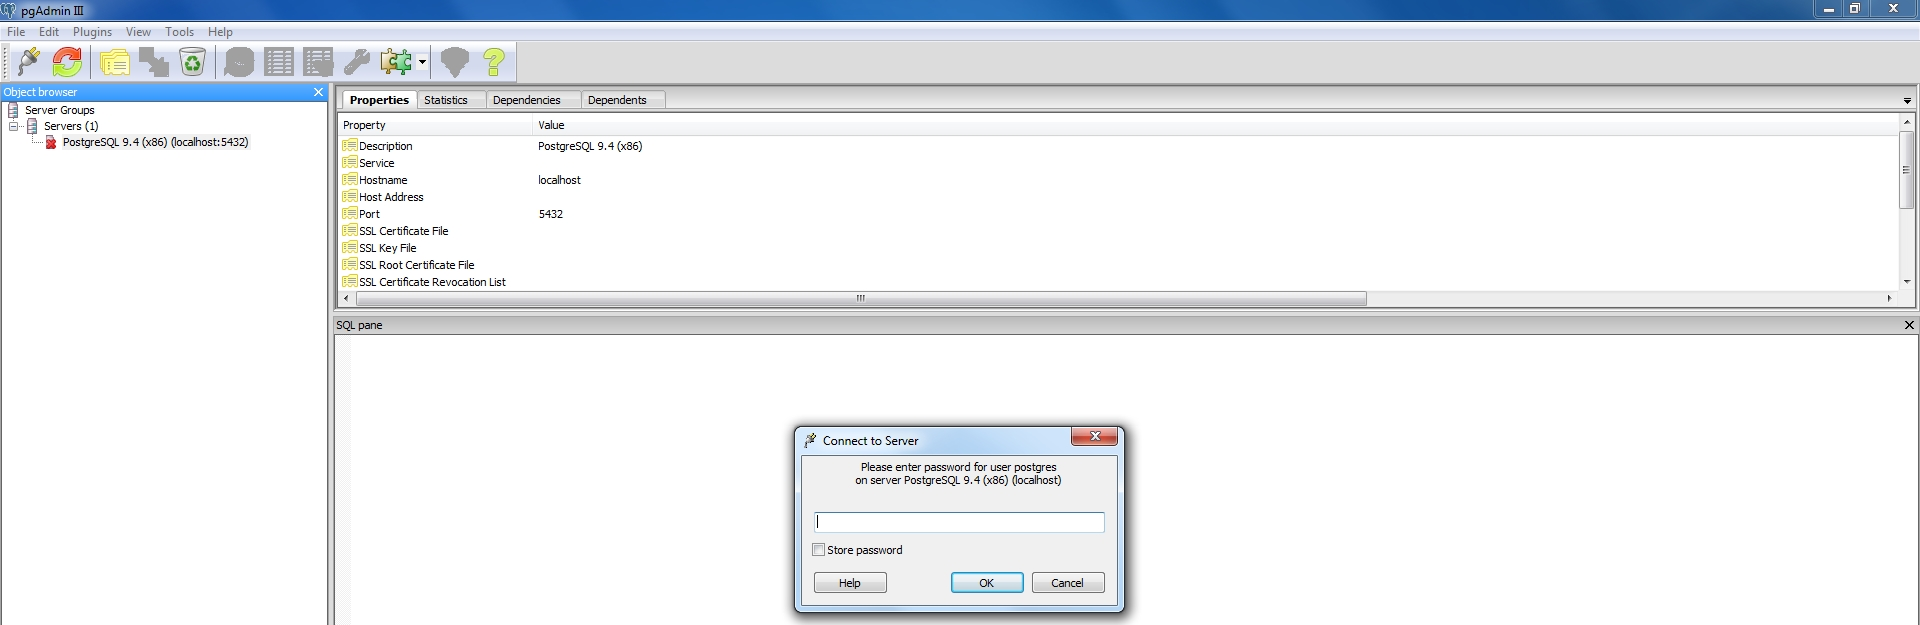
\includegraphics[width=1\linewidth]{./img/pgadmin-acceso.jpg}
\caption[]{Acceso al servidor\label{fig:pgadmin-acceso}}
\end{figure}

\newpage

Haga click derecho en el men\'{u} <<Login Roles>> y seleccione la opci\'{o}n <<New Login Role...>> (v\'{e}ase la figura \ref{fig:pgadmin-rol}).

\begin{figure}[H]
  \centering
  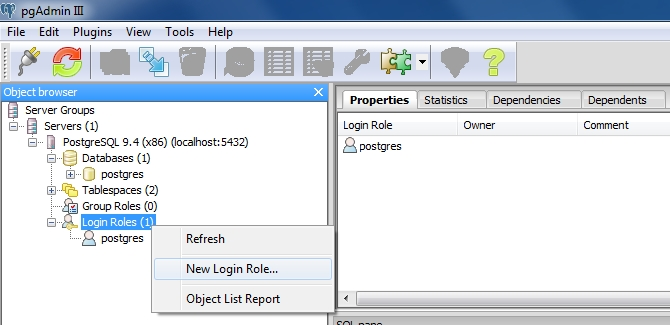
\includegraphics[width=1\linewidth]{./img/pgadmin-rol.jpg}
\caption[]{Crear nuevo rol\label{fig:pgadmin-rol}}
\end{figure}

Introduzca <<CIMBUC>> en <<Role name>> (v\'{e}ase la figura \ref{fig:pgadmin-rol-nombre}).

\begin{figure}[H]
  \centering
  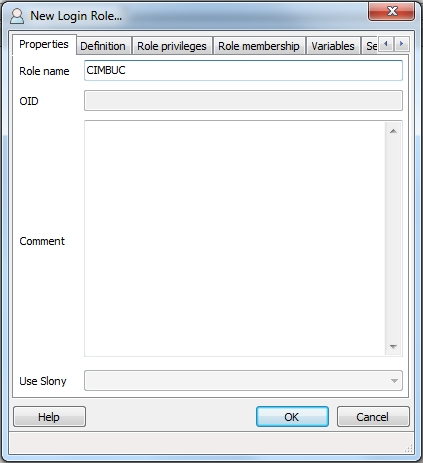
\includegraphics[width=.5\linewidth]{./img/pgadmin-rol-nombre.jpg}
\caption[]{Nombre del rol\label{fig:pgadmin-rol-nombre}}
\end{figure}

Haga click en la pesta\~{n}a <<Definition>> e introduzca <<CIMBUC>> como la contrase\~{n}a del rol (v\'{e}ase la figura \ref{fig:pgadmin-rol-clave}).

\begin{figure}[H]
  \centering
  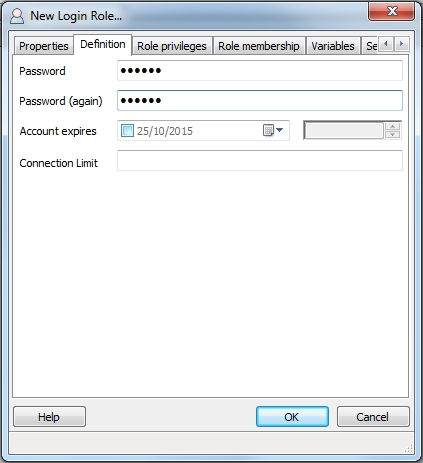
\includegraphics[width=.45\linewidth]{./img/pgadmin-rol-clave.jpg}
\caption[]{Contrase\~{n}a del rol\label{fig:pgadmin-rol-clave}}
\end{figure}

Haga click en la pesta\~{n}a <<Role privileges>>, seleccione todas las opciones de privilegios disponibles para el rol y haga click en el bot\'{o}n <<OK>> (v\'{e}ase la figura \ref{fig:pgadmin-rol-privilegios}).

\begin{figure}[H]
  \centering
  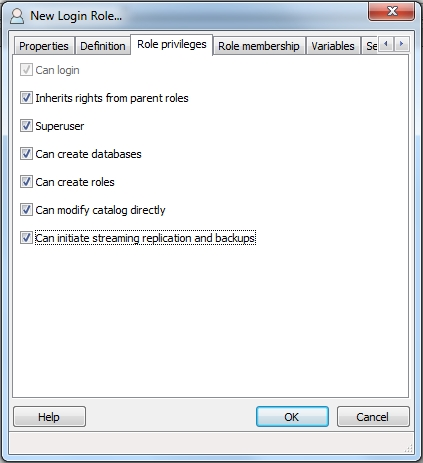
\includegraphics[width=.45\linewidth]{./img/pgadmin-rol-privilegios.jpg}
\caption[]{Privilegios del rol\label{fig:pgadmin-rol-privilegios}}
\end{figure}

\newpage

Haga click derecho en el men\'{u} <<Databases>> y seleccione la opci\'{o}n <<New Database...>> (v\'{e}ase la figura \ref{fig:pgadmin-bd}).

\begin{figure}[H]
  \centering
  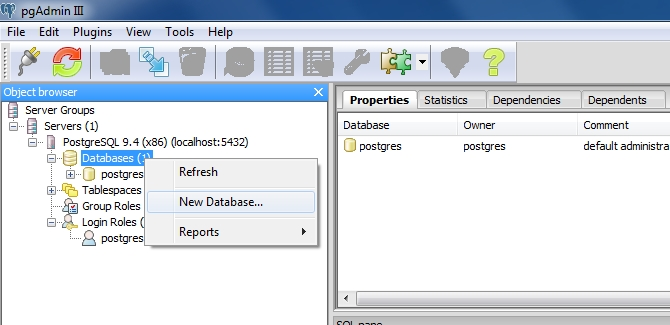
\includegraphics[width=1\linewidth]{./img/pgadmin-bd.jpg}
\caption[]{Crear nueva base de datos\label{fig:pgadmin-bd}}
\end{figure}

Introduzca <<CIMBUC>> en <<Name>> y haga click en el bot\'{o}n <<OK>> (v\'{e}ase la figura \ref{fig:pgadmin-bd-nombre}).

\begin{figure}[H]
  \centering
  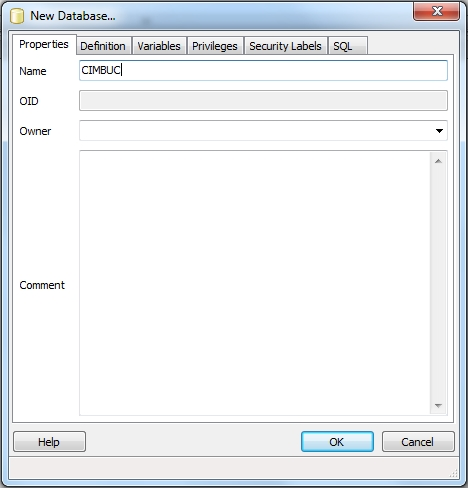
\includegraphics[width=.5\linewidth]{./img/pgadmin-bd-nombre.jpg}
\caption[]{Nombre de la base de datos\label{fig:pgadmin-bd-nombre}}
\end{figure}

\newpage

Haga click derecho en la base de datos <<CIMBUC>> y seleccione la opci\'{o}n <<Restore...>> (v\'{e}ase la figura \ref{fig:pgadmin-restaurar}).

\begin{figure}[H]
  \centering
  \includegraphics[width=1\linewidth]{./img/pgadmin-restaurar.jpg}
\caption[]{Opci\'{o}n de restauraci\'{o}n de la base de datos\label{fig:pgadmin-restaurar}}
\end{figure}

\newpage

Haga click en el bot\'{o}n <<...>> para buscar el archivo de respaldo de la base de datos (v\'{e}ase la figura \ref{fig:pgadmin-restaurar-ventana}).

\begin{figure}[H]
  \centering
  \includegraphics[width=.6\linewidth]{./img/pgadmin-restaurar-ventana.jpg}
\caption[]{Ventana de restauraci\'{o}n de la base de datos\label{fig:pgadmin-restaurar-ventana}}
\end{figure}

Busque y seleccione el archivo <<spectradb.backup>>, y haga click en el bot\'{o}n <<Abrir>> (v\'{e}ase la figura \ref{fig:pgadmin-restaurar-buscar}).

\begin{figure}[H]
  \centering
  \includegraphics[width=1\linewidth]{./img/pgadmin-restaurar-buscar.jpg}
\caption[]{Buscar el archivo de respaldo\label{fig:pgadmin-restaurar-buscar}}
\end{figure}

\newpage

De vuelta a la ventana de restauraci\'{o}n, haga click en la lista desplegable de <<Rolename>> y seleccione la opci\'{o}n <<CIMBUC>> (v\'{e}ase la figura \ref{fig:pgadmin-restaurar-rol}).

\begin{figure}[H]
  \centering
  \includegraphics[width=.6\linewidth]{./img/pgadmin-restaurar-rol.jpg}
\caption[]{Rol de restauraci\'{o}n de la base de datos\label{fig:pgadmin-restaurar-rol}}
\end{figure}

Haga click en la pesta\~{n}a <<Restore Options \#1>> y en el grupo <<Sections>> seleccione las opciones <<Pre-data>>, <<Data>> y <<Post-data>>, luego haga click en el bot\'{o}n <<Restore>> (v\'{e}ase la figura \ref{fig:pgadmin-restaurar-opciones}).

\begin{figure}[H]
  \centering
  \includegraphics[width=.6\linewidth]{./img/pgadmin-restaurar-opciones.jpg}
\caption[]{Opciones de restauraci\'{o}n de la base de datos\label{fig:pgadmin-restaurar-opciones}}
\end{figure}

\newpage

En la misma ventana haga click en bot\'{o}n <<Done>>, y por \'{u}ltimo cierre el software pgAdmin (v\'{e}ase la figura \ref{fig:pgadmin-restaurar-listo}).

\begin{figure}[H]
  \centering
  \includegraphics[width=.6\linewidth]{./img/pgadmin-restaurar-listo.jpg}
\caption[]{Restauraci\'{o}n de la base de datos completa\label{fig:pgadmin-restaurar-listo}}
\end{figure}

Es importante destacar que los pasos seguidos previamente s\'{o}lo se deben realizar una vez, y no es necesario que ejecute pgAdmin posteriormente para ejecutar el Spectrasoft.

La base de datos posee un usuario administrador por defecto para iniciar sesi\'{o}n y trabajar con el Spectrasoft, sus datos de ingreso son los siguientes: 

\begin{itemize}
	\item \textbf{C\'{e}dula de identidad:} V00000000
	
	\item \textbf{Contrase\~{n}a:} 12345Admin
\end{itemize}

Luego de iniciar sesi\'{o}n en el Spectrasoft con este usuario, puede crear otro usuario administrador de su preferencia y eliminar este.

\section*{Instalaci\'{o}n del Spectrasoft}

Ejecute el instalador <<setup-spectrasoft>> y haga click en el bot\'{o}n <<Next>>, dejando todas las opciones por defecto hasta llegar al acuerdo de licencia (v\'{e}ase la figura \ref{fig:spectrasoft-setup}).

\begin{figure}[H]
  \centering
  \includegraphics[width=.5\linewidth]{./img/spectrasoft-setup.jpg}
\caption[]{Instalador del Spectrasoft\label{fig:spectrasoft-setup}}
\end{figure}

En la ventana <<License Agreement>>, seleccione la opci\'{o}n <<I accept the license>> y haga click en el bot\'{o}n <<Next>> (v\'{e}ase la figura \ref{fig:spectrasoft-licencia}). Deje las siguientes opciones por defecto hasta llegar la opci\'{o}n de instalar.

\begin{figure}[H]
  \centering
  \includegraphics[width=.5\linewidth]{./img/spectrasoft-licencia.jpg}
\caption[]{Licencia del Spectrasoft\label{fig:spectrasoft-licencia}}
\end{figure}

\newpage

En la ventana <<Ready to Install>> haga click en el bot\'{o}n <<Install>> (v\'{e}ase la figura \ref{fig:spectrasoft-instalar}).

\begin{figure}[H]
  \centering
  \includegraphics[width=.6\linewidth]{./img/spectrasoft-instalar.jpg}
\caption[]{Instalar el Spectrasoft\label{fig:spectrasoft-instalar}}
\end{figure}

En la ventana <<Completing the Spectrasoft Wizard>> haga click en el bot\'{o}n <<Finish>> (v\'{e}ase la figura \ref{fig:spectrasoft-finalizar}).

\begin{figure}[H]
  \centering
  \includegraphics[width=.6\linewidth]{./img/spectrasoft-finalizar.jpg}
\caption[]{Finalizar la instalaci\'{o}n\label{fig:spectrasoft-finalizar}}
\end{figure}

\newpage

Por \'{u}ltimo, para ejecutar el Spectrasoft abra el men\'{u} de inicio de Windows y haga click en la opci\'{o}n <<Spectrasoft>> (v\'{e}ase la figura \ref{fig:spectrasoft-ejecutable}).

\begin{figure}[H]
  \centering
  \includegraphics[width=.4\linewidth]{./img/spectrasoft-ejecutable.jpg}
\caption[]{Ejecutar el Spectrasoft\label{fig:spectrasoft-ejecutable}}
\end{figure}

Si desea entrar al men\'{u} del Spectrasoft, abra el men\'{u} de inicio de Windows, haga click en la opci\'{o}n <<Todos los programas>>, busque la carpeta llamada <<Spectrasoft>> y seleccionela (v\'{e}ase la figura \ref{fig:spectrasoft-menu}).

\begin{figure}[H]
  \centering
  \includegraphics[width=.4\linewidth]{./img/spectrasoft-menu.jpg}
\caption[]{Men\'{u} del Spectrasoft\label{fig:spectrasoft-menu}}
\end{figure}
\newpage
%%%%%%%%%%%%%%%%%%%%%%
%%%%%%%%%%%%%%%%%%%%%%
\chapter{Manual de usuario}
\thispagestyle{fancy}
\vfill
\section*{Introducci\'{o}n}
	El Spectrasoft es un software de c\'{o}digo abierto para el manejo del MiniScan XE Plus, el cual es usado en el diagn\'{o}stico de patolog\'{i}as dermatol\'{o}gicas en pacientes. Este software ofrece funciones de gesti\'{o}n de mediciones, historias m\'{e}dicas de pacientes y muestras. La vista principal del Spectrasoft es la mostrada en la figura \ref{fig:vista-principal}.

\begin{figure}[H]
  \centering
  \includegraphics[width=1\linewidth]{./img/vista-principal.jpg}
\caption[]{Vista principal del Spectrasoft\label{fig:vista-principal}}
\end{figure}
\vfill
\newpage

\section*{Permisolog\'{i}a de los usuarios}

	Spectrasoft maneja tres roles de usuario: administradores, dermat\'{o}logos e investigadores. Si bien los tres roles comparten acciones comunes que pueden realizar, cada uno tiene permisos diferentes que lo distinguen de los dem\'{a}s. Estos permisos son descritos en la tabla 1.

\begin{table}[h]
		\small
		\caption[]{Permisolog\'{i}a de los usuarios}
		\centering
		\setlength{\extrarowheight}{\altocelda}
		\begin{tabulary}{\anchotabla}{|c|J|}
			\hline
			\thead{\textbf{\small{Usuario}}} & \thead{\textbf{\small{Permisos}}}\\ \hline
			
			\textbf{Administrador} &
			
			Manejar el MiniScan XE Plus.
			
			Registrar, buscar, modificar y eliminar usuarios.
			
			Buscar y ver historias m\'{e}dicas de pacientes.
			
			Buscar y ver muestras de pacientes.\\ \hline
			
			\textbf{Dermat\'{o}logo} &
			
			Manejar el MiniScan XE Plus.
			
			Registrar, buscar, ver, modificar y eliminar historias m\'{e}dicas de pacientes.
			
			Registrar, buscar, ver, modificar y eliminar muestras de pacientes.\\ \hline
			
			\textbf{Investigador} &
			
			Manejar el MiniScan XE Plus.
			
			Buscar y ver historias m\'{e}dicas de pacientes.
			
			Buscar y ver muestras de pacientes.\\ \hline
		\end{tabulary}
	\end{table}

	Es importante destacar que todas las operaciones de registro, modificaci\'{o}n y eliminaci\'{o}n requieren de la contrase\~{n}a del usuario responsable de dicha operaci\'{o}n.
	
\newpage

\section*{Manejo del MiniScan XE Plus}

	\subsection*{Conectar y desconectar}
		Para conectar o desconectar el MiniScan XE Plus, entre al men\'{u} del MiniScan (v\'{e}ase la figura \ref{fig:conectar-desconectar}).

\begin{figure}[H]
\centering
\begin{subfigure}{.5\textwidth}
  \centering
  \includegraphics[width=.6\linewidth]{./img/conectar.jpg}
\end{subfigure}%
\begin{subfigure}{.5\textwidth}
  \centering
  \includegraphics[width=.6\linewidth]{./img/desconectar.jpg}
\end{subfigure}
\caption[]{Conectar y desconectar MiniScan XE Plus\label{fig:conectar-desconectar}}
\end{figure}

	\subsection*{Calibrar}
		Entre al men\'{u} del Miniscan y seleccione la opci\'{o}n estandarizar. Prepare la trampa negra del Miniscan para su medici\'{o}n y seleccione listo, por \'{u}ltimo prepare la cer\'{a}mica blanca para su medici\'{o}n y seleccione listo (v\'{e}ase la figura \ref{fig:calibrar}).
	
\begin{figure}[H]
\centering
\begin{subfigure}{.33\textwidth}
  \centering
  \includegraphics[width=.9\linewidth]{./img/estandarizar.jpg}
\end{subfigure}%
\centering
\begin{subfigure}{.33\textwidth}
  \centering
  \includegraphics[width=.9\linewidth]{./img/estandarizar-negro.jpg}
\end{subfigure}%
\begin{subfigure}{.33\textwidth}
  \centering
  \includegraphics[width=.9\linewidth]{./img/estandarizar-blanco.jpg}
\end{subfigure}
\caption[]{Calibrar el MiniScan XE Plus\label{fig:calibrar}}
\end{figure}

\section*{Gesti\'{o}n de mediciones}
	
	\subsection*{Realizar una medici\'{o}n}
	
	Entre al men\'{u} del MiniScan, o bien seleccione la opci\'{o}n directamente de la barra de herramientras (v\'{e}ase la figura \ref{fig:medicion}).
	
\begin{figure}[H]
\centering
\begin{subfigure}{.5\textwidth}
  \centering
  \includegraphics[width=.6\linewidth]{./img/medir-menu.jpg}
\end{subfigure}%
\begin{subfigure}{.5\textwidth}
  \centering
  \includegraphics[width=.6\linewidth]{./img/medir-barra.jpg}
\end{subfigure}
\caption[]{Realizar medici\'{o}n\label{fig:medicion}}
\end{figure}

	\subsection*{Consultar resultados de una medici\'{o}n}
	
	El men\'{u} de los resultados de una medici\'{o}n es ilustrado en la figura \ref{fig:menu-resultados}, y todos los resultados son ilustrados desde la figura \ref{fig:datos-espectrales} a la figura \ref{fig:resultados-adicionales}.

\begin{figure}[H]
  \centering
  \includegraphics[width=.5\linewidth]{./img/resultados-menu.jpg}
\caption[]{Men\'{u} de resultados de una medici\'{o}n\label{fig:menu-resultados}}
\end{figure}

\begin{figure}[H]
  \centering
  \includegraphics[width=1\linewidth]{./img/resultados.jpg}
\caption[]{Datos espectrales de una medici\'{o}n\label{fig:datos-espectrales}}
\end{figure}

\begin{figure}[H]
  \centering
  \includegraphics[width=1\linewidth]{./img/resultados-reflectancia.jpg}
\caption[]{Curva de reflectancia de una medici\'{o}n\label{fig:resultados-reflectancia}}
\end{figure}

\newpage

\begin{figure}[H]
  \centering
  \includegraphics[width=1\linewidth]{./img/resultados-absorbancia.jpg}
\caption[]{Curva de absorbancia de una medici\'{o}n\label{fig:resultados-absorbancia}}
\end{figure}

\begin{figure}[H]
  \centering
  \includegraphics[width=1\linewidth]{./img/resultados-absorcion.jpg}
\caption[]{Curva de absorci\'{o}n de una medici\'{o}n\label{fig:resultados-absorcion}}
\end{figure}

\newpage
\null
\vfill
\begin{figure}[H]
  \centering
  \includegraphics[width=.6\linewidth]{./img/resultados-adicionales.jpg}
\caption[]{Datos adicionales de una medici\'{o}n\label{fig:resultados-adicionales}}
\end{figure}
\vfill
\newpage

\section*{Gesti\'{o}n de sesiones}

	\subsection*{Iniciar sesi\'{o}n}
	
	Para iniciar sesi\'{o}n entre al men\'{u} de usuario y seleccione la opci\'{o}n iniciar sesi\'{o}n. Debe ingresar su c\'{e}dula de identidad y su contrase\~{n}a. Esto es ilustrado en la figura \ref{fig:iniciar-sesion}.
	
\begin{figure}[H]
  \centering
  \includegraphics[width=1\linewidth]{./img/inicio-sesion.jpg}
\caption[]{Iniciar sesi\'{o}n\label{fig:iniciar-sesion}}
\end{figure}
	
	\subsection*{Ver informaci\'{o}n del usuario}
	
	Seleccione la opci\'{o}n ver usuario, ubicada en el men\'{u} de usuario. El men\'{u} de usuario y la ventana de informaci\'{o}n son ilustrados en las figuras \ref{fig:menu-usuario} y \ref{fig:ver-usuario}.
\newpage
\null
\vfill
\begin{figure}[H]
  \centering
  \includegraphics[width=.3\linewidth]{./img/menu-usuario.jpg}
\caption[]{Men\'{u} de usuario\label{fig:menu-usuario}}
\end{figure}

\begin{figure}[H]
  \centering
  \includegraphics[width=.5\linewidth]{./img/ver-usuario.jpg}
\caption[]{Ver usuario\label{fig:ver-usuario}}
\end{figure}
\vfill
\newpage

	\subsection*{Modificar informaci\'{o}n del usuario}

	Seleccione la opci\'{o}n modificar usuario, ubicada en el men\'{u} de usuario. La ventana para modificar el usuario es ilustrada en la figura \ref{fig:modificar-usuario}.

	\subsection*{Cambiar contrase\~{n}a del usuario}

	Seleccione la opci\'{o}n cambiar contrase\~{n}a, ubicada en el men\'{u} de usuario. Debe ingresar la contrase\~{n}a actual del usuario y la nueva contrase\~{n}a (dos veces) para poder realizar el cambio. La ventana para realizar esta operaci\'{o}n se ilustra en la figura \ref{fig:cambiar-clave}.

\begin{figure}[H]
\centering
\begin{minipage}{.5\textwidth}
  \centering
  \includegraphics[width=.9\linewidth]{./img/modificar-usuario.jpg}
  \captionof{figure}[]{Modificar usuario\label{fig:modificar-usuario}}
  \label{fig:test1}
\end{minipage}%
\begin{minipage}{.5\textwidth}
  \centering
  \includegraphics[width=.9\linewidth]{./img/cambiar-clave.jpg}
  \captionof{figure}[]{Cambiar contrase\~{n}a\label{fig:cambiar-clave}}
  \label{fig:test2}
\end{minipage}
\end{figure}

	\subsection*{Cerrar sesi\'{o}n}
	
	Seleccione la opci\'{o}n cerrar sesi\'{o}n, ubicada en el men\'{u} usuario.

\newpage

\section*{Gesti\'{o}n de historias}

	\subsection*{Registrar historia}
	
	Seleccione la opci\'{o}n registrar historia, ubicada en el men\'{u} historia. Solo los usuarios dermat\'{o}logos pueden registrar una historia m\'{e}dica. El men\'{u} de historia y la ventana de registro se ilustran en las figuras \ref{fig:menu-historia} y \ref{fig:registrar-historia}.

\begin{figure}[H]
  \centering
  \includegraphics[width=.3\linewidth]{./img/menu-historia.jpg}
\caption[]{Men\'{u} historia\label{fig:menu-historia}}
\end{figure}

\begin{figure}[H]
  \centering
  \includegraphics[width=.4\linewidth]{./img/registrar-historia.jpg}
\caption[]{Resgistrar historia\label{fig:registrar-historia}}
\end{figure}

	\subsection*{Buscar historia}
	
	En el men\'{u} de historia, seleccione la opci\'{o}n buscar historia. Esta ventana permite filtrar la b\'{u}squeda de historias empleando ciertos criterios. Para abrir la historia, seleccionela en la lista de historias y por \'{u}ltimo seleccione la opci\'{o}n abrir historia. Esta ventana se ilustra en la figura \ref{fig:buscar-historia}.
	
\begin{figure}[H]
  \centering
  \includegraphics[width=.9\linewidth]{./img/buscar-historia.jpg}
\caption[]{Buscar historia\label{fig:buscar-historia}}
\end{figure}
	
	\subsection*{Ver historia}
	
	Seleccione la opci\'{o}n ver historia, ubicada en el men\'{u} historia. Esta ventana es ilustrada en la figura \ref{fig:ver-historia}.
	
\begin{figure}[H]
  \centering
  \includegraphics[width=.5\linewidth]{./img/ver-historia1.jpg}
\caption[]{Ver historia\label{fig:ver-historia}}
\end{figure}
\newpage
	\subsection*{Modificar historia}
	
	Seleccione la opci\'{o}n modificar historia, ubicada en el submen\'{u} m\'{a}s opciones, dentro del men\'{u} historia. Esta ventana se ilustra en la figura \ref{fig:modificar-historia}.
	
	\subsection*{Eliminar historia}
	
	Seleccione la opci\'{o}n eliminar historia, ubicada en el submen\'{u} m\'{a}s opciones, dentro del men\'{u} historia. Esta ventana se ilustra en la figura \ref{fig:eliminar-historia}.
	
\begin{figure}[H]
\centering
\begin{minipage}{.5\textwidth}
  \centering
  \includegraphics[width=.9\linewidth]{./img/modificar-historia.jpg}
  \captionof{figure}[]{Modificar historia}
  \label{fig:modificar-historia}
\end{minipage}%
\begin{minipage}{.5\textwidth}
  \centering
  \includegraphics[width=1\linewidth]{./img/eliminar-historia.jpg}
  \captionof{figure}[]{Eliminar historia}
  \label{fig:eliminar-historia}
\end{minipage}
\end{figure}

	\subsection*{Cerrar historia}
	
	Seleccione la opci\'{o}n cerrar historia, ubicada en el men\'{u} historia.

\newpage

\section*{Gesti\'{o}n de muestras}

	\subsection*{Registrar muestra}
	
	Seleccione la opci\'{o}n registrar muestra, ubicada en el men\'{u} de muestra (tambi\'{e}n disponible en la barra de herramientas). En la ventana de registro aparecer\'{a}n dos tipos de muestra que se pueden registrar, fototipo y lesi\'{o}n. Solo se puede registrar una muestra si el usuario es dermat\'{o}logo, si hay una historia m\'{e}dica cargada y si se realiz\'{o} una medici\'{o}n nueva. El men\'{u} muestra y la ventana de tipos de muestra se ilustran en las figuras \ref{fig:menu-muestra} y \ref{fig:tipos-muestra}.
	
\begin{figure}[H]
  \centering
  \includegraphics[width=.3\linewidth]{./img/menu-muestra.jpg}
\caption[]{Men\'{u} muestra\label{fig:menu-muestra}}
\end{figure}

\begin{figure}[H]
  \centering
  \includegraphics[width=.8\linewidth]{./img/tipo-muestra.jpg}
\caption[]{Tipos de muestra\label{fig:tipos-muestra}}
\end{figure}
	
		\subsubsection*{Registrar fototipo}
		
		En la ventana para registrar un fototipo, debe especificar el \'{a}rea en donde se le est\'{a} tomando la muestra al paciente, y se debe seleccionar el fototipo, en la opci\'{o}n clasificar fototipo. Esta ventana se puede apreciar en la figura \ref{fig:registrar-fototipo}.
		
\begin{figure}[H]
  \centering
  \includegraphics[width=.5\linewidth]{./img/registrar-fototipo1.jpg}
\caption[]{Registrar fototipo\label{fig:registrar-fototipo}}
\end{figure}

		En la ventana de clasificaci\'{o}n del fototipo aparecer\'{a} el fototipo recomendado para la muestra dada, y ser\'{a} necesario elegir el fototipo que se desea registrar. Esto es ilustrado en la figura \ref{fig:clasificar-fototipo}.
\newpage
\null
\vfill
\begin{figure}[H]
  \centering
  \includegraphics[width=.8\linewidth]{./img/fototipo.jpg}
\caption[]{Clasificar fototipo\label{fig:clasificar-fototipo}}
\end{figure}
\vfill
\newpage
	Luego de haber elegido el fototipo, aparecer\'{a} la ventana de registro nuevamente, con el fototipo elegido actualizado; por \'{u}ltimo, seleccione registrar fototipo. Esto es ilustrado en la figura \ref{fig:registrar-fototipo2}.

\begin{figure}[H]
  \centering
  \includegraphics[width=.5\linewidth]{./img/registrar-fototipo2.jpg}
\caption[]{Registrar fototipo\label{fig:registrar-fototipo2}}
\end{figure}
\newpage	

\subsubsection*{Registrar lesi\'{o}n}
			En la ventana de registrar lesi\'{o}n, debe especificar el nombre de la lesi\'{o}n y el \'{a}rea en donde se est\'{a} tomando la muestra de la misma. Esta ventana se puede apreciar en la figura \ref{fig:registrar-lesion}.
		
\begin{figure}[H]
  \centering
  \includegraphics[width=.6\linewidth]{./img/registrar-lesion.jpg}
\caption[]{Registrar lesi\'{o}n\label{fig:registrar-lesion}}
\end{figure}
\newpage
	\subsection*{Buscar muestra}

		Seleccione la opci\'{o}n buscar muestra, ubicada en el men\'{u} de muestra (tambi\'{e}n disponible en la barra de herramientas). Esta ventana permite filtrar la b\'{u}squeda de las muestras pertenecientes a la historia que est\'{e} cargada en ese momento, empleando ciertos criterios. Para abrir la muestra, seleccionela en la lista de muestras y por \'{u}ltimo seleccione la opci\'{o}n abrir muestra. Esta ventana se ilustra en la figura \ref{fig:buscar-muestra}.

\begin{figure}[H]
  \centering
  \includegraphics[width=.9\linewidth]{./img/buscar-muestra.jpg}
\caption[]{Buscar muestra\label{fig:buscar-muestra}}
\end{figure}
\newpage
	\subsection*{Ver muestra}
	
	Seleccione la opci\'{o}n ver muestra, ubicada en el men\'{u} de muestra (tambi\'{e}n disponible en la barra de herramientas). Esta ventana se ilustra en la figura \ref{fig:ver-muestra}.
	
\begin{figure}[H]
  \centering
  \includegraphics[width=.5\linewidth]{./img/ver-muestra.jpg}
\caption[]{Ver muestra\label{fig:ver-muestra}}
\end{figure}
\newpage
	\subsection*{Exportar muestra}
	
	Seleccione la opci\'{o}n exportar muestra, ubicada en el men\'{u} de muestra (tambi\'{e}n disponible en la barra de herramientas). Estas opciones se ilustran en la figura \ref{fig:exportar-muestra}.
	
\begin{figure}[H]
\centering
\begin{subfigure}{.5\textwidth}
  \centering
  \includegraphics[width=.6\linewidth]{./img/exportar-menu.jpg}
\end{subfigure}%
\begin{subfigure}{.5\textwidth}
  \centering
  \includegraphics[width=.45\linewidth]{./img/exportar-barra.jpg}
\end{subfigure}
\caption[]{Exportar muestra\label{fig:exportar-muestra}}
\end{figure}

	La muestra se exporta en el escritorio a un archivo .xlsx, que puede abrirse y modificarse con cualquier programa que maneje hojas de c\'{a}lculo.

	\subsection*{Modificar muestra}
	
	Seleccione la opci\'{o}n modificar muestra, ubicada en el submen\'{u} m\'{a}s opciones, dentro del men\'{u} muestra. Esta ventana se ilustra en la figura \ref{fig:modificar-muestra}.
\newpage
	\subsection*{Eliminar muestra}
	
	Seleccione la opci\'{o}n eliminar muestra, ubicada en el submen\'{u} m\'{a}s opciones, dentro del men\'{u} muestra. Esta ventana se ilustra en la figura \ref{fig:eliminar-muestra}.
	
\begin{figure}[H]
\centering
\begin{minipage}{.5\textwidth}
  \centering
  \includegraphics[width=.9\linewidth]{./img/modificar-muestra.jpg}
  \captionof{figure}[]{Modificar muestra}
  \label{fig:modificar-muestra}
\end{minipage}%
\begin{minipage}{.5\textwidth}
  \centering
  \includegraphics[width=1\linewidth]{./img/eliminar-muestra.jpg}
  \captionof{figure}[]{Eliminar muestra}
  \label{fig:eliminar-muestra}
\end{minipage}
\end{figure}

	\subsection*{Cerrar muestra}
	
	Seleccione la opci\'{o}n cerrar muestra, ubicada en el men\'{u} muestra.

\newpage

\section*{Gesti\'{o}n de usuarios}

	\subsection*{Registrar usuario}
	
	Seleccione la opci\'{o}n registrar usuario, ubicada en el submen\'{u} m\'{a}s opciones, dentro del men\'{u} usuario. Esta ventana es ilustrada en la figura \ref{fig:registrar-usuario}.
	
\begin{figure}[H]
  \centering
  \includegraphics[width=.6\linewidth]{./img/registrar-usuario.jpg}
\caption[]{Registrar usuario\label{fig:registrar-usuario}}
\end{figure}
	
	\subsection*{Administrar usuarios}
	
	Seleccione la opci\'{o}n administrar usuarios, ubicada en el submen\'{u} m\'{a}s opciones, dentro del men\'{u} usuario. Administrar usuarios permite cambiar sus roles, cambiar sus contrase\~{n}as y eliminarlos. Esta ventana es ilustrada en la figura \ref{fig:administrar-usuarios}.
	
\begin{figure}[H]
  \centering
  \includegraphics[width=1\linewidth]{./img/administrar-usuarios.jpg}
\caption[]{Administrar usuarios\label{fig:administrar-usuarios}}
\end{figure}
	
		\subsubsection*{Cambiar rol}
		
		Una vez haya seleccionado un usuario de la lista de usuarios, seleccione la opci\'{o}n cambiar rol. Esta ventana es ilustrada en la figura \ref{fig:cambiar-rol}.
		
\begin{figure}[H]
  \centering
  \includegraphics[width=1\linewidth]{./img/administrar-rol.jpg}
\caption[]{Cambiar rol\label{fig:cambiar-rol}}
\end{figure}
\newpage
		\subsubsection*{Cambiar contrase\~{n}a}
		
		Una vez haya seleccionado un usuario de la lista de usuarios, seleccione la opci\'{o}n cambiar contrase\~{n}a. Esta opci\'{o}n requiere de la contrase\~{n}a del administrador que este realizando la operaci\'{o}n, y de la nueva contrase\~{n}a para el usuario. Esto es ilustrado en la figura \ref{fig:cambiar-clave2}.
		
\begin{figure}[H]
  \centering
  \includegraphics[width=1\linewidth]{./img/administrar-clave.jpg}
\caption[]{Cambiar contrase\~{n}a\label{fig:cambiar-clave2}}
\end{figure}
\newpage
		\subsubsection*{Eliminar usuario}
		
		Una vez haya seleccionado un usuario de la lista de usuarios, seleccione la opci\'{o}n eliminar usuario. Esta opci\'{o}n solo se puede realizar con usuarios que no sean administradores. Esta opci\'{o}n es ilustrada en la figura \ref{fig:eliminar-usuario}.
		
\begin{figure}[H]
  \centering
  \includegraphics[width=1\linewidth]{./img/administrar-eliminar.jpg}
\caption[]{Eliminar usuario\label{fig:eliminar-usuario}}
\end{figure}
\newpage
%%%%%%%%%%%%%%%%%%%%%%%%%%%
%%%%%%%%%%%%%%%%%%%%%%%%%%%
\renewcommand{\anchotabla}{16.5cm}
\renewcommand{\altocelda}{2pt}
{\renewcommand\normalsize{\small}
\normalsize
\newgeometry{top=2.5cm, bottom=3cm, left=2.5cm,right=2cm}
\fontsize{10pt}{10pt}\selectfont
\chapter{Guiones de prueba}
\thispagestyle{fancy}
\begin{center}
	\textbf{Gui\'{o}n de prueba 1}
\end{center}

\textbf{Nombre del proyecto:} \proyecto

\textbf{\'{A}rea funcional:} Operaci\'{o}n del MiniScan XE Plus.

\textbf{Nombre de la prueba:} Operar el MiniScan XE Plus.
\vfill
\textbf{Prop\'{o}sito:}
\begin{table}[h]
	\centering
	\setlength{\extrarowheight}{\altocelda}
	\begin{tabularx}{\anchotabla}{|X|}
		\hline
		Probar la funcionalidad que implica operar el MiniScan XE Plus.\\ \hline
	\end{tabularx}
\end{table}

\textbf{Resultado:}
\begin{table}[h]
	\centering
	\setlength{\extrarowheight}{\altocelda}
	\begin{tabularx}{\anchotabla}{|X|}
		\hline
		Prueba superada con \'{e}xito.\\ \hline
	\end{tabularx}
\end{table}

\begin{table}[h]
		\centering
		\setlength{\extrarowheight}{\altocelda}
		\begin{tabulary}{\anchotabla}{|c|J|J|J|}
			\hline
			\thead{\textbf{\small{\#}}} & \thead{\textbf{\small{Acci\'{o}n}}} & \thead{\textbf{\small{Opci\'{o}n}}} & \thead{\textbf{\small{Resultado esperado}}}\\ \hline

			1 & El usuario conecta el software con el MiniScan. & Se selecciona la opci\'{o}n <<Conectar>>, ubicada en el men\'{u} MiniScan. & Ventana de confirmaci\'{o}n, informando al usuario que la conexi\'{o}n ha sido establecida.\\ \hline
			
			2 & El usuario realiza una medici\'{o}n. & Se selecciona la opci\'{o}n <<Realizar medici\'{o}n>>, ubicada en el men\'{u} MiniScan. & Tabla de datos espectrales recuperados de la medici\'{o}n.\\ \hline
		
			3 & El usuario desconecta el software con el MiniScan. & Se selecciona la opci\'{o}n <<Desconectar>>, ubicada en el men\'{u} MiniScan. & Ventana de confirmaci\'{o}n, informando al usuario que la desconexi\'{o}n ha sido realizada.\\ \hline
			
			4 & El usuario calibra el MiniScan. & Se selecciona la opci\'{o}n <<Estandarizar>>, ubicada en el men\'{u} MiniScan. & Ventanas de calibraci\'{o}n para la trampa negra y la cer\'{a}mica blanca del MiniScan.\\ \hline
		\end{tabulary}
\end{table}
\newpage
\textbf{Errores encontrados:}
\begin{table}[H]
	\centering
	\setlength{\extrarowheight}{\altocelda}
	\begin{tabularx}{\anchotabla}{|X|}
		\hline
		\thead{\textbf{\small{Descripci\'{o}n del error}}}
		\\ \hline
		No se encontr\'{o} ning\'{u}n error.\\ \hline
	\end{tabularx}
\end{table}

\textbf{Comentarios y observaciones:}
\begin{table}[H]
	\centering
	\setlength{\extrarowheight}{\altocelda}
	\begin{tabularx}{\anchotabla}{|X|}
		\hline
		Se verific\'{o} la funcionalidad desconectando f\'{i}sicamente el MiniScan, en cuyo caso el software genera un mensaje de error al usuario.\\ \hline
	\end{tabularx}
\end{table}

\begin{minipage}[t]{0.45\textwidth}
	\begin{flushleft}
		\textbf{Elaborado por:} \nombre
	\end{flushleft}
\end{minipage}
\begin{minipage}[t]{0.45\textwidth}
	\begin{flushright}
		\begin{center}
			\textbf{Fecha:} \fecha
		\end{center}
	\end{flushright}
\end{minipage}
\vfill
\newpage
\begin{center}
	\textbf{Gui\'{o}n de prueba 2}
\end{center}

\textbf{Nombre del proyecto:} \proyecto

\textbf{\'{A}rea funcional:} Resultados.

\textbf{Nombre de la prueba:} Gestionar resultados.
\vfill
\textbf{Prop\'{o}sito:}
\begin{table}[h]
	\centering
	\setlength{\extrarowheight}{\altocelda}
	\begin{tabularx}{\anchotabla}{|X|}
		\hline
		Probar la funcionalidad que implica gestionar los resultados de las mediciones.\\ \hline
	\end{tabularx}
\end{table}

\textbf{Resultado:}
\begin{table}[h]
	\centering
	\setlength{\extrarowheight}{\altocelda}
	\begin{tabularx}{\anchotabla}{|X|}
		\hline
		Prueba superada con \'{e}xito.\\ \hline
	\end{tabularx}
\end{table}

\begin{table}[h]
		\centering
		\setlength{\extrarowheight}{\altocelda}
		\begin{tabulary}{\anchotabla}{|c|J|J|J|}
			\hline
			\thead{\textbf{\small{\#}}} & \thead{\textbf{\small{Acci\'{o}n}}} & \thead{\textbf{\small{Opci\'{o}n}}} & \thead{\textbf{\small{Resultado esperado}}}\\ \hline

			1 & El usuario consulta los resultados de una medici\'{o}n. & Se selecciona los resultados disponibles en el men\'{u} Resultados. & Ventanas con los resultados adicionales de una medici\'{o}n.\\ \hline
		
			2 & El usuario borra los resultados de una medici\'{o}n. & Se selecciona la opci\'{o}n <<Borrar resultados>>, ubicada en el men\'{u} resultados. & Ventana de confirmaci\'{o}n, informando al usuario que se han borrado los resultados correctamente.\\ \hline
		\end{tabulary}
\end{table}

\textbf{Errores encontrados:}
\begin{table}[H]
	\centering
	\setlength{\extrarowheight}{\altocelda}
	\begin{tabularx}{\anchotabla}{|X|}
		\hline
		\thead{\textbf{\small{Descripci\'{o}n del error}}}
		\\ \hline
		No se encontr\'{o} ning\'{u}n error.\\ \hline
	\end{tabularx}
\end{table}

\textbf{Comentarios y observaciones:}
\begin{table}[H]
	\centering
	\setlength{\extrarowheight}{\altocelda}
	\begin{tabularx}{\anchotabla}{|X|}
		\hline
		No aplica.\\ \hline
	\end{tabularx}
\end{table}

\begin{minipage}[t]{0.45\textwidth}
	\begin{flushleft}
		\textbf{Elaborado por:} \nombre
	\end{flushleft}
\end{minipage}
\begin{minipage}[t]{0.45\textwidth}
	\begin{flushright}
		\begin{center}
			\textbf{Fecha:} \fecha
		\end{center}
	\end{flushright}
\end{minipage}
\vfill
\newpage
\begin{center}
	\textbf{Gui\'{o}n de prueba 3}
\end{center}

\textbf{Nombre del proyecto:} \proyecto

\textbf{\'{A}rea funcional:} Sesi\'{o}n de usuarios.

\textbf{Nombre de la prueba:} Gestionar sesi\'{o}n de usuarios.
\vfill
\textbf{Prop\'{o}sito:}
\begin{table}[h]
	\centering
	\setlength{\extrarowheight}{\altocelda}
	\begin{tabularx}{\anchotabla}{|X|}
		\hline
		Probar la funcionalidad que implica gestionar la sesi\'{o}n de un usuario.\\ \hline
	\end{tabularx}
\end{table}

\textbf{Resultado:}
\begin{table}[h]
	\centering
	\setlength{\extrarowheight}{\altocelda}
	\begin{tabularx}{\anchotabla}{|X|}
		\hline
		Prueba superada con \'{e}xito.\\ \hline
	\end{tabularx}
\end{table}

\begin{table}[h]
		\centering
		\setlength{\extrarowheight}{\altocelda}
		\begin{tabulary}{\anchotabla}{|c|J|J|J|}
			\hline
			\thead{\textbf{\small{\#}}} & \thead{\textbf{\small{Acci\'{o}n}}} & \thead{\textbf{\small{Opci\'{o}n}}} & \thead{\textbf{\small{Resultado esperado}}}\\ \hline

			1 & El usuario inicia su sesi\'{o}n, suministrando su c\'{e}dula de identidad y su contrase\~{n}a. & Se selecciona la opci\'{o}n <<Iniciar sesi\'{o}n>>, ubicada en el men\'{u} usuario. & Ventana de confirmaci\'{o}n, informando al usuario que ha iniciado sesi\'{o}n correctamente.\\ \hline
		
			2 & El usuario ve sus datos personales. & Se selecciona la opci\'{o}n <<Ver usuario>>, ubicada en el men\'{u} usuario. & Ventana de muestra los datos personales del usuario.\\ \hline
			
			3 & El usuario modifica sus datos personales, proporcionando su contrase\~{n}a. & Se selecciona la opci\'{o}n <<Modificar usuario>>, ubicada en el men\'{u} usuario. & Ventana de confirmaci\'{o}n, informando al usuario que ha modificado sus datos correctamente.\\ \hline
			
			4 & El usuario cambia su contrase\~{n}a, proporcionando su contrase\~{n}a actual y su contrase\~{n}a nueva. & Se selecciona la opci\'{o}n <<Cambiar contrase\~{n}a>>, ubicada en el men\'{u} usuario. & Ventana de confirmaci\'{o}n, informando al usuario que ha cambiado su contrase\~{n}a correctamente.\\ \hline
			
			5 & El usuario cierra su sesi\'{o}n. & Se selecciona la opci\'{o}n <<Cerrar sesi\'{o}n>>, ubicada en el men\'{u} usuario. & Ventana de confirmaci\'{o}n, informando al usuario que ha cerrado su sesi\'{o}n correctamente.\\ \hline
		\end{tabulary}
\end{table}
\vfill
\newpage
\textbf{Errores encontrados:}
\begin{table}[H]
	\centering
	\setlength{\extrarowheight}{\altocelda}
	\begin{tabularx}{\anchotabla}{|X|}
		\hline
		\thead{\textbf{\small{Descripci\'{o}n del error}}}
		\\ \hline
		No se encontr\'{o} ning\'{u}n error.\\ \hline
	\end{tabularx}
\end{table}

\textbf{Comentarios y observaciones:}
\begin{table}[H]
	\centering
	\setlength{\extrarowheight}{\altocelda}
	\begin{tabularx}{\anchotabla}{|X|}
		\hline
		Se verific\'{o} la funcionalidad proporcionando una contrase\~{n}a incorrecta en las operaciones de inicio de sesi\'{o}n y modificaci\'{o}n, en cuyo caso el software genera un mensaje de error al usuario.\\ \hline
	\end{tabularx}
\end{table}

\begin{minipage}[t]{0.45\textwidth}
	\begin{flushleft}
		\textbf{Elaborado por:} \nombre
	\end{flushleft}
\end{minipage}
\begin{minipage}[t]{0.45\textwidth}
	\begin{flushright}
		\begin{center}
			\textbf{Fecha:} \fecha
		\end{center}
	\end{flushright}
\end{minipage}
\vfill
\newpage
\begin{center}
	\textbf{Gui\'{o}n de prueba 4}
\end{center}

\textbf{Nombre del proyecto:} \proyecto

\textbf{\'{A}rea funcional:} Historias.

\textbf{Nombre de la prueba:} Gestionar historias.
\vfill
\textbf{Prop\'{o}sito:}
\begin{table}[h]
	\centering
	\setlength{\extrarowheight}{\altocelda}
	\begin{tabularx}{\anchotabla}{|X|}
		\hline
		Probar la funcionalidad que implica gestionar las historias m\'{e}dicas.\\ \hline
	\end{tabularx}
\end{table}

\textbf{Resultado:}
\begin{table}[h]
	\centering
	\setlength{\extrarowheight}{\altocelda}
	\begin{tabularx}{\anchotabla}{|X|}
		\hline
		Prueba superada con \'{e}xito.\\ \hline
	\end{tabularx}
\end{table}

\begin{table}[h]
		\centering
		\setlength{\extrarowheight}{\altocelda}
		\begin{tabulary}{\anchotabla}{|c|J|J|J|}
			\hline
			\thead{\textbf{\small{\#}}} & \thead{\textbf{\small{Acci\'{o}n}}} & \thead{\textbf{\small{Opci\'{o}n}}} & \thead{\textbf{\small{Resultado esperado}}}\\ \hline

			1 & El usuario registra una historia, suministrando datos personales del paciente y su contrase\~{n}a de usuario. & Se selecciona la opci\'{o}n <<Registrar historia>>, ubicada en el men\'{u} historia. & Ventana de confirmaci\'{o}n, informando al usuario que ha registrado la historia correctamente.\\ \hline
		
			2 & El usuario busca una historia existente. & Se selecciona la opci\'{o}n <<Buscar historia>>, ubicada en el men\'{u} historia. & Ventana de confirmaci\'{o}n, informando al usuario que ha abierto la historia correctamente.\\ \hline
			
			3 & El usuario ve los datos de la historia. & Se selecciona la opci\'{o}n <<Ver historia>>, ubicada en el men\'{u} historia. & Ventana de muestra los datos de la historia m\'{e}dica.\\ \hline
			
			4 & El usuario modifica los datos de la historia, proporcionando su contrase\~{n}a de usuario. & Se selecciona la opci\'{o}n <<Modificar historia>>, ubicada en el men\'{u} historia. & Ventana de confirmaci\'{o}n, informando al usuario que ha modificado la historia correctamente.\\ \hline
			
			5 & El usuario cierra la historia. & Se selecciona la opci\'{o}n <<Cerrar historia>>, ubicada en el men\'{u} historia. & Ventana de confirmaci\'{o}n, informando al usuario que ha cerrado la historia correctamente.\\ \hline
			
			6 & El usuario elimina la historia, proporcionando su contrase\~{n}a de usuario. & Se selecciona la opci\'{o}n <<Eliminar historia>>, ubicada en el men\'{u} historia. & Ventana de confirmaci\'{o}n, informando al usuario que ha eliminado la historia correctamente.\\ \hline
		\end{tabulary}
\end{table}
\newpage
\textbf{Errores encontrados:}
\begin{table}[H]
	\centering
	\setlength{\extrarowheight}{\altocelda}
	\begin{tabularx}{\anchotabla}{|X|}
		\hline
		\thead{\textbf{\small{Descripci\'{o}n del error}}}
		\\ \hline
		No se encontr\'{o} ning\'{u}n error.\\ \hline
	\end{tabularx}
\end{table}

\textbf{Comentarios y observaciones:}
\begin{table}[H]
	\centering
	\setlength{\extrarowheight}{\altocelda}
	\begin{tabularx}{\anchotabla}{|X|}
		\hline
		Se verific\'{o} la funcionalidad proporcionando una contrase\~{n}a incorrecta en las operaciones de registro, modificaci\'{o}n y eliminaci\'{o}n, en cuyo caso el software genera un mensaje de error al usuario.\\ \hline
	\end{tabularx}
\end{table}

\begin{minipage}[t]{0.45\textwidth}
	\begin{flushleft}
		\textbf{Elaborado por:} \nombre
	\end{flushleft}
\end{minipage}
\begin{minipage}[t]{0.45\textwidth}
	\begin{flushright}
		\begin{center}
			\textbf{Fecha:} \fecha
		\end{center}
	\end{flushright}
\end{minipage}
\vfill
\newpage
\begin{center}
	\textbf{Gui\'{o}n de prueba 5}
\end{center}

\textbf{Nombre del proyecto:} \proyecto

\textbf{\'{A}rea funcional:} Muestras.

\textbf{Nombre de la prueba:} Gestionar muestras.

\textbf{Prop\'{o}sito:}
\begin{table}[h]
	\centering
	\setlength{\extrarowheight}{\altocelda}
	\begin{tabularx}{\anchotabla}{|X|}
		\hline
		Probar la funcionalidad que implica gestionar muestras.\\ \hline
	\end{tabularx}
\end{table}

\textbf{Resultado:}
\begin{table}[h]
	\centering
	\setlength{\extrarowheight}{\altocelda}
	\begin{tabularx}{\anchotabla}{|X|}
		\hline
		Prueba superada con \'{e}xito.\\ \hline
	\end{tabularx}
\end{table}
\begin{table}[h]
		\centering
		\setlength{\extrarowheight}{\altocelda}
		\begin{tabulary}{\anchotabla}{|c|J|J|J|}
			\hline
			\thead{\textbf{\small{\#}}} & \thead{\textbf{\small{Acci\'{o}n}}} & \thead{\textbf{\small{Opci\'{o}n}}} & \thead{\textbf{\small{Resultado esperado}}}\\ \hline

			1 & El usuario registra una muestra, suministrando los datos de la misma y su contrase\~{n}a de usuario. & Se selecciona la opci\'{o}n <<Registrar muestra>>, ubicada en el men\'{u} muestra. & Ventana de confirmaci\'{o}n, informando al usuario que ha registrado la muestra correctamente.\\ \hline
		
			2 & El usuario busca una muestra existente. & Se selecciona la opci\'{o}n <<Buscar muestra>>, ubicada en el men\'{u} muestra. & Ventana de confirmaci\'{o}n, informando al usuario que ha abierto la muestra correctamente.\\ \hline
			
			3 & El usuario ve los datos de la muestra. & Se selecciona la opci\'{o}n <<Ver muestra>>, ubicada en el men\'{u} muestra. & Ventana que proporciona los datos de la muestra.\\ \hline
			
			4 & El usuario exporta los datos de la muestra. & Se selecciona la opci\'{o}n <<Exportar muestra>>, ubicada en el men\'{u} muestra. & Ventana de confirmaci\'{o}n, informando al usuario que ha exportado la muestra correctamente.\\ \hline
			
			5 & El usuario modifica los datos de la muestra, proporcionando su contrase\~{n}a de usuario. & Se selecciona la opci\'{o}n <<Modificar muestra>>, ubicada en el men\'{u} muestra. & Ventana de confirmaci\'{o}n, informando al usuario que ha modificado la muestra correctamente.\\ \hline
			
			6 & El usuario cierra la muestra. & Se selecciona la opci\'{o}n <<Cerrar muestra>>, ubicada en el men\'{u} muestra. & Ventana de confirmaci\'{o}n, informando al usuario que ha cerrado la muestra correctamente.\\ \hline
			
			7 & El usuario elimina la muestra, proporcionando su contrase\~{n}a de usuario. & Se selecciona la opci\'{o}n <<Eliminar muestra>>, ubicada en el men\'{u} muestra. & Ventana de confirmaci\'{o}n, informando al usuario que ha eliminado la muestra correctamente.\\ \hline
		\end{tabulary}
\end{table}
\FloatBarrier
\newpage
\textbf{Errores encontrados:}
\begin{table}[H]
	\centering
	\setlength{\extrarowheight}{\altocelda}
	\begin{tabularx}{\anchotabla}{|X|}
		\hline
		\thead{\textbf{\small{Descripci\'{o}n del error}}}
		\\ \hline
		No se encontr\'{o} ning\'{u}n error.\\ \hline
	\end{tabularx}
\end{table}

\textbf{Comentarios y observaciones:}
\begin{table}[H]
	\centering
	\setlength{\extrarowheight}{\altocelda}
	\begin{tabularx}{\anchotabla}{|X|}
		\hline
		Se verific\'{o} la funcionalidad proporcionando una contrase\~{n}a incorrecta en las operaciones de registro, modificaci\'{o}n y eliminaci\'{o}n, en cuyo caso el software genera un mensaje de error al usuario.\\ \hline
	\end{tabularx}
\end{table}

\begin{minipage}[t]{0.45\textwidth}
	\begin{flushleft}
		\textbf{Elaborado por:} \nombre
	\end{flushleft}
\end{minipage}
\begin{minipage}[t]{0.45\textwidth}
	\begin{flushright}
		\begin{center}
			\textbf{Fecha:} \fecha
		\end{center}
	\end{flushright}
\end{minipage}
\vfill
\newpage
\begin{center}
	\textbf{Gui\'{o}n de prueba 6}
\end{center}

\textbf{Nombre del proyecto:} \proyecto

\textbf{\'{A}rea funcional:} Administraci\'{o}n de usuarios.

\textbf{Nombre de la prueba:} Gestionar usuarios.
\vfill
\textbf{Prop\'{o}sito:}
\begin{table}[h]
	\centering
	\setlength{\extrarowheight}{\altocelda}
	\begin{tabularx}{\anchotabla}{|X|}
		\hline
		Probar la funcionalidad que implica gestionar usuarios.\\ \hline
	\end{tabularx}
\end{table}

\textbf{Resultado:}
\begin{table}[h]
	\centering
	\setlength{\extrarowheight}{\altocelda}
	\begin{tabularx}{\anchotabla}{|X|}
		\hline
		Prueba superada con \'{e}xito.\\ \hline
	\end{tabularx}
\end{table}

\begin{table}[h]
		\centering
		\setlength{\extrarowheight}{\altocelda}
		\begin{tabulary}{\anchotabla}{|c|J|J|J|}
			\hline
			\thead{\textbf{\small{\#}}} & \thead{\textbf{\small{Acci\'{o}n}}} & \thead{\textbf{\small{Opci\'{o}n}}} & \thead{\textbf{\small{Resultado esperado}}}\\ \hline

			1 & El administrador registra un usuario, suministrando los datos personales del mismo y su contrase\~{n}a de administrador. & Se selecciona la opci\'{o}n <<Registrar usuario>>, ubicada en el men\'{u} usuario. & Ventana de confirmaci\'{o}n, informando al administrador que ha registrado al nuevo usuario correctamente.\\ \hline
		
			2 & El administrador gestiona un usuario existente. & Se selecciona la opci\'{o}n <<Administrar usuarios>>, ubicada en el men\'{u} usuario. & Ventana de administraci\'{o}n de usuarios.\\ \hline
			
			3 & El administrador ve los datos de un usuario. & Se selecciona la opci\'{o}n <<Ver usuario>>, ubicada en la ventana administrar usuarios. & Ventana que muestra los datos del usuario.\\ \hline
			
			4 & El administrador cambia el rol de un usuario, proporcionando su contrase\~{n}a de administrador. & Se selecciona la opci\'{o}n <<Cambiar rol>>, ubicada en la ventana administrar usuarios. & Ventana de confirmaci\'{o}n, informando al administrador que ha cambiado el rol del usuario correctamente.\\ \hline
			
			5 & El administrador cambia la contrase\~{n}a de un usuario, proporcionando su contrase\~{n}a de administrador. & Se selecciona la opci\'{o}n <<Cambiar contrase\~{n}a>>, ubicada en la ventana administrar usuario. & Ventana de confirmaci\'{o}n, informando al administrador que ha cambiado la contrase\~{n}a del usuario correctamente.\\ \hline
			
			6 & El administrador elimina un usuario, proporcionando su contrase\~{n}a de administrador. & Se selecciona la opci\'{o}n <<Eliminar usuario>>, ubicada en la ventana administrar usuarios. & Ventana de confirmaci\'{o}n, informando al administrador que ha eliminado al usuario correctamente.\\ \hline
		\end{tabulary}
\end{table}
\newpage
\textbf{Errores encontrados:}
\begin{table}[H]
	\centering
	\setlength{\extrarowheight}{\altocelda}
	\begin{tabularx}{\anchotabla}{|X|}
		\hline
		\thead{\textbf{\small{Descripci\'{o}n del error}}}
		\\ \hline
		No se encontr\'{o} ning\'{u}n error.\\ \hline
	\end{tabularx}
\end{table}

\textbf{Comentarios y observaciones:}
\begin{table}[H]
	\centering
	\setlength{\extrarowheight}{\altocelda}
	\begin{tabularx}{\anchotabla}{|X|}
		\hline
		Se verific\'{o} la funcionalidad proporcionando una contrase\~{n}a incorrecta en las operaciones de cambio de rol, cambio de contrase\~{n}a y eliminaci\'{o}n, en cuyo caso el software genera un mensaje de error al administrador.\\ \hline
	\end{tabularx}
\end{table}

\begin{minipage}[t]{0.45\textwidth}
	\begin{flushleft}
		\textbf{Elaborado por:} \nombre
	\end{flushleft}
\end{minipage}
\begin{minipage}[t]{0.45\textwidth}
	\begin{flushright}
		\begin{center}
			\textbf{Fecha:} \fecha
		\end{center}
	\end{flushright}
\end{minipage}
\vfill
\newpage
%%%%%%%%%%%%%%%%%%%%%%%%%%%%%%%
%%%%%%%%%%%%%%%%%%%%%%%%%%%%%%%
\chapter{Pruebas de aceptaci\'{o}n}
\thispagestyle{fancy}
\begin{center}
	\textbf{Prueba de aceptaci\'{o}n}
\end{center}

\textbf{Nombre del proyecto:} \proyecto

\textbf{Usuario:} Dermat\'{o}logo.

\textbf{Prop\'{o}sito:}
\begin{table}[h]
	\centering
	\setlength{\extrarowheight}{\altocelda}
	\begin{tabularx}{\anchotabla}{|X|}
		\hline
		Evaluar el cumplimiento y la satisfacci\'{o}n de los requerimientos establecidos durante la definici\'{o}n del proyecto.\\ \hline
	\end{tabularx}
\end{table}

\textbf{Resultado:}
\begin{table}[h]
	\centering
	\setlength{\extrarowheight}{\altocelda}
	\begin{tabulary}{\anchotabla}{|c|L|J|c|}
		\hline
		\thead{\textbf{\small{\#}}} & \thead{\textbf{\small{Requerimiento}}} & \thead{\textbf{\small{Acci\'{o}n}}} & \thead{\textbf{\small{Resultado}}}\\ \hline

			1 & Conectar el \hbox{MiniScan}. & Conectar el software con el MiniScan. & \'{E}xito \\ \hline
		
			2 & Desconectar el \hbox{MiniScan}. & Desconectar el software del MiniScan. & \'{E}xito \\ \hline
			
			3 & Calibrar el \hbox{MiniScan}. & Calibrar el MiniScan, utilizando una trampa de luz y una cer\'{a}mica blanca. & \'{E}xito \\ \hline
			
			4 & Realizar una medici\'{o}n. & Realizar una medici\'{o}n con el MiniScan. & \'{E}xito \\ \hline
			
			5 & Consultar resultados. & Consultar los resultados de una medici\'{o}n realizada. & \'{E}xito \\ \hline
			
			6 & Borrar resultados. & Borrar los resultados obtenidos de una medici\'{o}n realizada. & \'{E}xito \\ \hline
			
			7 & Iniciar sesi\'{o}n. & Iniciar la sesi\'{o}n de usuario. & \'{E}xito \\ \hline
			
			8 & Consultar usuario. & Consultar los datos personales del usuario. & \'{E}xito \\ \hline
			
			9 & Modificar usuario. & Modificar los datos personales del usuario. & \'{E}xito \\ \hline
			
			10 & Cerrar sesi\'{o}n. & Cerrar la sesi\'{o}n de usuario. & \'{E}xito \\ \hline
			
			11 & Registrar historia. & Registrar la historia m\'{e}dica de un paciente. & \'{E}xito \\ \hline
			
			12 & Consultar historia. & Consultar los datos de la historia m\'{e}dica de un paciente. & \'{E}xito \\ \hline
			
			13 & Modificar historia. & Modificar los datos de la historia m\'{e}dica de un paciente. & \'{E}xito \\ \hline
			
			14 & Cerrar historia. & Cerrar la historia m\'{e}dica de un paciente. & \'{E}xito \\ \hline
			
			15 & Eliminar historia. & Eliminar la historia m\'{e}dica de un paciente. & \'{E}xito \\ \hline
			
			16 & Registrar muestra. & Registrar una muestra perteneciente a una historia. & \'{E}xito \\ \hline
			
			17 & Consultar muestra. & Consultar los datos de una muestra perteneciente a una historia. & \'{E}xito \\ \hline
			
			18 & Exportar muestra. & Exportar los datos de una muestra a un archivo port\'{a}til. & \'{E}xito \\ \hline

	\end{tabulary}
\end{table}

\begin{table}[h]
		\centering
		\setlength{\extrarowheight}{\altocelda}
		\begin{tabulary}{\anchotabla}{|c|L|J|c|}
			\hline
			\thead{\textbf{\small{\#}}} & \thead{\textbf{\small{Requerimiento}}} & \thead{\textbf{\small{Acci\'{o}n}}} & \thead{\textbf{\small{Resultado}}}\\ \hline
	
			19 & Modificar muestra. & Modificar los datos de una muestra perteneciente a una historia. & \'{E}xito \\ \hline
			
			20 & Cerrar muestra. & Cerrar una muestra perteneciente a una historia. & \'{E}xito \\ \hline
			
			21 & Eliminar muestra. & Eliminar una muestra perteneciente a una historia. & \'{E}xito \\ \hline
	
	\end{tabulary}
\end{table}

\FloatBarrier
\textbf{Comentarios y observaciones:}
\begin{table}[H]
	\centering
	\setlength{\extrarowheight}{\altocelda}
	\begin{tabularx}{\anchotabla}{|X|}
		\hline
		No aplica.	
		\\ \hline
	\end{tabularx}
\end{table}

\begin{minipage}[t]{0.45\textwidth}
	\begin{flushleft}
		\textbf{Elaborado por:} Sandra Vivas.
	\end{flushleft}
\end{minipage}
\begin{minipage}[t]{0.45\textwidth}
	\begin{flushright}
		\begin{center}
			\textbf{Fecha:} 20 de octubre, 2015.
		\end{center}
	\end{flushright}
\end{minipage}
\vfill

\newpage
\begin{center}
	\textbf{Constancia de prueba de aceptaci\'{o}n}
\end{center}

Por medio de la presente, se hace constar que el cliente Sandra Vivas, luego de una reuni\'{o}n realizada el 20 de octubre de 2015, donde se presentaron y probaron las diferentes funcionalidades del software Spectrasoft, ha manifestado su satisfacci\'{o}n y ha aceptado su producto. En virtud de lo cual, firma la presente constancia de aceptaci\'{o}n, junto con el desarrollador.

\null
\null
\null

\begin{minipage}[t]{0.45\textwidth}
	\begin{flushleft}
		\begin{center}
			\textbf{Cliente}
		\end{center}
	\end{flushleft}
\end{minipage}
\begin{minipage}[t]{0.45\textwidth}
	\begin{flushright}
		\begin{center}
			\textbf{Desarrollador}
		\end{center}
	\end{flushright}
\end{minipage}
\newpage
%%%%%%%%%%%%%%%%%%%%%%%%%%%%%%%%%%%%%%%%%%%%%%%%%%%%%%%%%%%%%%%%%%%%%%
%%%%%%%%%%%%%%%%%%%%%%%%%%%%%%%%%%%%%%%%%%%%%%%%%%%%%%%%%%%%%%%%%%%%%%
\begin{center}
	\textbf{Prueba de aceptaci\'{o}n}
\end{center}

\textbf{Nombre del proyecto:} \proyecto

\textbf{Usuario:} Investigador.

\textbf{Prop\'{o}sito:}
\begin{table}[h]
	\centering
	\setlength{\extrarowheight}{\altocelda}
	\begin{tabularx}{\anchotabla}{|X|}
		\hline
		Evaluar el cumplimiento y la satisfacci\'{o}n de los requerimientos establecidos durante la definici\'{o}n del proyecto.\\ \hline
	\end{tabularx}
\end{table}

\textbf{Resultado:}

\begin{table}[h]
	\centering
	\setlength{\extrarowheight}{\altocelda}
	\begin{tabulary}{\anchotabla}{|c|L|J|c|}
		\hline
		\thead{\textbf{\small{\#}}} & \thead{\textbf{\small{Requerimiento}}} & \thead{\textbf{\small{Acci\'{o}n}}} & \thead{\textbf{\small{Resultado}}}\\ \hline

			1 & Conectar el \hbox{MiniScan}. & Conectar el software con el MiniScan. & \'{E}xito \\ \hline
		
			2 & Desconectar el \hbox{MiniScan}. & Desconectar el software del MiniScan. & \'{E}xito \\ \hline
			
			3 & Calibrar el \hbox{MiniScan}. & Calibrar el MiniScan, utilizando una trampa de luz y una cer\'{a}mica blanca. & \'{E}xito \\ \hline
			
			4 & Realizar una medici\'{o}n. & Realizar una medici\'{o}n con el MiniScan. & \'{E}xito \\ \hline
			
			5 & Consultar resultados. & Consultar los resultados de una medici\'{o}n realizada. & \'{E}xito \\ \hline
			
			6 & Borrar resultados. & Borrar los resultados obtenidos de una medici\'{o}n realizada. & \'{E}xito \\ \hline
			
			7 & Iniciar sesi\'{o}n. & Iniciar la sesi\'{o}n de usuario. & \'{E}xito \\ \hline
			
			8 & Consultar usuario. & Consultar los datos personales del usuario. & \'{E}xito \\ \hline
			
			9 & Modificar usuario. & Modificar los datos personales del usuario. & \'{E}xito \\ \hline
			
			10 & Cerrar sesi\'{o}n. & Cerrar la sesi\'{o}n de usuario. & \'{E}xito \\ \hline
			
			11 & Consultar historia. & Consultar los datos de la historia m\'{e}dica de un paciente. & \'{E}xito \\ \hline
			
			12 & Cerrar historia. & Cerrar la historia m\'{e}dica de un paciente. & \'{E}xito \\ \hline
			
			13 & Consultar muestra. & Consultar los datos de una muestra perteneciente a una historia. & \'{E}xito \\ \hline
			
			14 & Exportar muestra. & Exportar los datos de una muestra a un archivo port\'{a}til. & \'{E}xito \\ \hline
			
			15 & Cerrar muestra. & Cerrar una muestra perteneciente a una historia. & \'{E}xito \\ \hline

	\end{tabulary}
\end{table}
\newpage
\FloatBarrier
\textbf{Comentarios y observaciones:}
\begin{table}[H]
	\centering
	\setlength{\extrarowheight}{\altocelda}
	\begin{tabularx}{\anchotabla}{|X|}
		\hline
		No aplica.
		\\ \hline
	\end{tabularx}
\end{table}

\begin{minipage}[t]{0.45\textwidth}
	\begin{flushleft}
		\textbf{Elaborado por:} Aar\'{o}n Mu\~{n}oz.
	\end{flushleft}
\end{minipage}
\begin{minipage}[t]{0.45\textwidth}
	\begin{flushright}
		\begin{center}
			\textbf{Fecha:} 20 de octubre, 2015.
		\end{center}
	\end{flushright}
\end{minipage}
\vfill

\newpage
\begin{center}
	\textbf{Constancia de prueba de aceptaci\'{o}n}
\end{center}

Por medio de la presente, se hace constar que el cliente Aar\'{o}n Mu\~{n}oz, luego de una reuni\'{o}n realizada el 20 de octubre de 2015, donde se presentaron y probaron las diferentes funcionalidades del software Spectrasoft, ha manifestado su satisfacci\'{o}n y ha aceptado su producto. En virtud de lo cual, firma la presente constancia de aceptaci\'{o}n, junto con el desarrollador.

\null
\null
\null

\begin{minipage}[t]{0.45\textwidth}
	\begin{flushleft}
		\begin{center}
			\textbf{Cliente}
		\end{center}
	\end{flushleft}
\end{minipage}
\begin{minipage}[t]{0.45\textwidth}
	\begin{flushright}
		\begin{center}
			\textbf{Desarrollador}
		\end{center}
	\end{flushright}
\end{minipage}
\newpage
	
\end{document}